\documentclass[11pt]{article}
\usepackage[T1]{fontenc}
\usepackage[utf8]{inputenc}
\usepackage{lmodern}
\usepackage[margin=1in]{geometry}
\usepackage{amsmath,amssymb,amsthm,mathtools}
\usepackage{booktabs,longtable,array}
\usepackage{graphicx}
\usepackage[numbers,sort&compress]{natbib}
\usepackage{xcolor}
\usepackage[hidelinks]{hyperref}
\usepackage[nameinlink,noabbrev]{cleveref}
\usepackage{microtype}
\newtheorem{theorem}{Theorem}[section]
\newtheorem{lemma}[theorem]{Lemma}
\newtheorem{proposition}[theorem]{Proposition}
\newtheorem{corollary}[theorem]{Corollary}
\theoremstyle{definition}
\newtheorem{definition}[theorem]{Definition}
\newtheorem{assumption}[theorem]{Assumption}
\newtheorem{example}[theorem]{Example}
\theoremstyle{remark}
\newtheorem{remark}[theorem]{Remark}
\newcommand{\R}{\mathbb R}
\newcommand{\Q}{\mathbb Q}
\newcommand{\Z}{\mathbb Z}
\newcommand{\N}{\mathbb N}
\newcommand{\eps}{\varepsilon}
\newcommand{\trans}{^{\mathsf T}}
\newcommand{\norm}[1]{\left\lVert#1\right\rVert}
\newcommand{\abs}[1]{\left\lvert#1\right\rvert}
\newcommand{\poly}{\operatorname{poly}}
\DeclareMathOperator{\argmin}{arg\,min}
\DeclareMathOperator{\argmax}{arg\,max}
\DeclareMathOperator{\diag}{diag}
\DeclareMathOperator{\clip}{clip}
\DeclareMathOperator{\dist}{dist}
\DeclareMathOperator{\rank}{rank}
\DeclareMathOperator{\conv}{conv}
\DeclareMathOperator{\sgn}{sgn}
\title{Structured bilevel optimization with many follower variables:\\
Global responses, accuracy, and structural boundaries}
\author{}
\date{}
\begin{document}
\maketitle
\begin{abstract}
We study continuous bilevel optimization in which many follower variables
interact only through a fixed number of shared resource rows and aggregate
quantities. For positive-definite quadratic follower blocks of fixed size
and a polynomial, possibly nonconvex aggregate cost, local elimination
followed by a global value comparison describes all globally optimal
follower responses in a fixed number of leader, aggregate and multiplier
coordinates, with only polynomially many realizable joint regimes. With
these dimensions fixed, exact algorithms polynomial in input length and
numerical degree decide optimistic and pessimistic feasibility, compute
exact infima, decide attainment and return optimizers in one
real-algebraic field, while the numbers of follower variables and upper
constraints may grow. The approach extends to robustness against
cost-near-optimal followers when each upper criterion uses a fixed number
of affine measurements. For strictly convex polynomial local costs and a
convex aggregate, we compute rational leaders with global additive error
$2^{-B}$ in time polynomial in input length, numerical degree and $B$;
response-dependent upper constraints receive outer and inner guarantees.
Exact optimization is NP-hard even with one leader and a dense
positive-definite follower Hessian arbitrarily close to the identity, and
output-length bounds show that numerical degrees cannot be replaced by
their bit lengths. Exact scalar implementations agree with an independent
original-coordinate baseline on all tested instances; certified dense
screening was slower than a numerical MILP comparator on every tested
instance.
\end{abstract}
\noindent\textbf{Keywords:} bilevel optimization; global optimization;
parametric quadratic programming; separable optimization; bit complexity;
near-optimal robustness.
\section{Introduction and problem setting}\label{sec:foundations}

Many leader--follower models contain many local follower choices but only
a few shared resources, aggregate quantities and leader decisions. A tariff
may influence the operation of many units whose nonlinear interaction
depends only on total load or emissions; a local variable or small block
describes the choices of one unit. We model one follower that
optimizes the joint allocation. This also covers separate agents whose
decisions decouple, but a nonconvex aggregate term does not in general
describe a Nash equilibrium among independent agents.

We ask whether the number of shared quantities, rather than the number of
follower variables, can control the complexity of \emph{global} bilevel
optimization. Linear bilevel optimization is strongly
NP-hard~\cite{HansenJaumardSavard1992}; see also~\cite{Buchheim2023,KetkovProkopyev2026}.
A linear class remains NP-complete with a single leader
variable~\cite{SugishitaCarvalhoIPCO2026,SugishitaCarvalho2026}. Positive
results fix the number of follower
variables~\cite{LiuSpencer1995,Deng1998,KetkovProkopyev2026} or, for linear
followers, the number of follower constraints~\cite{KetkovProkopyev2026}. A tractable follower
problem does not suffice: the leader optimizes over the responses induced
by all its decisions, and this problem can be nonconvex even when every
follower has a unique convex minimizer. Standard single-level
reformulations do not answer the question either. A KKT reformulation
replaces follower optimality by stationarity. This is exact for convex
followers under a constraint qualification, which linear constraints such
as ours satisfy, but for nonconvex followers stationary points need not be
global optima; its mixed-integer form also needs valid big-$M$
bounds~\cite{KleinertEtAl2021,Buchheim2023}.
A value-function reformulation is exact for nonconvex followers but
quantifies over the entire follower vector~\cite{JeyakumarEtAl2016,NieWangYe2017}.
We therefore separate three tasks: describing all global follower
responses, optimizing over them under a stated optimistic or pessimistic
selection convention, and representing the output at a stated accuracy.

\paragraph{Key idea.}
In the model of \cref{subsec:model}, fix a leader $x$ and an aggregate
value $w=U(x)z$. On the fiber $\{z\in P(x):U(x)z=w\}$ the aggregate cost is
constant and the remaining local cost is strictly convex, so a global
follower optimum is the unique minimizer on its own fiber. With multipliers
for the $k$ shared rows, each block becomes a small strictly convex
parametric quadratic program whose solution is piecewise rational in the
compressed coordinates $\zeta=(x,w,\lambda,\mu)\in\R^{r+s+k}$, with
polynomially many branches per block. We call
$r+s+k$ the \emph{response description dimension}. Only polynomially many
joint regimes of all blocks are realizable in this fixed dimension, and a
value-function comparison in the compressed coordinates, rather than in all
$N$ follower variables, selects exactly the global responses.

\subsection{Contributions and scope}\label{subsec:contributions}

Under explicit local structure, a large follower dimension can thus be
replaced by a fixed response description dimension. Our original
contributions are the combined complexity and recovery guarantees
below, together with the restriction-preserving boundary constructions.
Degrees are numerical degrees, and exponents may depend on the fixed
dimensions (\cref{subsec:encoding}).

\paragraph{Exact global responses (\cref{sec:exact}).}
The follower has positive-definite quadratic local blocks of fixed
dimension $d$, $k$ shared linear rows, and a polynomial, possibly nonconvex
cost of $s$ aggregates; the leader has $r$ variables. The numbers of
blocks, local rows and upper polynomial rows, and the supports of the upper
polynomials, can grow. For fixed $(r,d,s,k)$, \cref{thm:exact-block}
decides optimistic feasibility and returns an attained optimizer and its
value in one real-algebraic field of polynomial encoding length, in time
polynomial in the input length and numerical degree. \Cref{thm:exact-semantics}
extends this to polynomially moving constraint normals and to pessimistic
selection with universal upper feasibility, computing exact infima and
deciding attainment. Fixed normals give optimistic attainment
(\cref{lem:closed-response}); moving normals or pessimistic selection can
lose it (\cref{ex:moving-nonattainment,ex:pessimistic-nonattainment}).
With constant local Hessians and fixed input degree, the algebraic degree
of the output is independent of the number of follower variables, for
fixed normals (\cref{cor:constant-hessian-degree}) and, in the robust
setting, with constant local rows but moving shared and measurement normals
(\cref{cor:robust-degree}). For a
supplied diagonal-plus-fixed-rank Hessian and affine upper data, rational
linear programs suffice (\cref{cor:low-rank-lp}). \Cref{thm:fixed-core}
gives a related polyhedral elimination theorem, with recovery of all blocks
by one common convex combination of a few support tuples.

\paragraph{Near-optimality robustness (\cref{sec:robust-screening}).}
Cost-near-optimal followers need not be stationary, so we minimize on the
fibers of the affine measurements used by each upper criterion.
\Cref{thm:nearoptimal-robust} gives exact robust feasibility and
worst-objective optimization when every criterion uses at most a fixed
number $h$ of measurements, even if the combined measurement rank grows.
Without this bound, computing the worst value of one convex quadratic
criterion is NP-hard (\cref{prop:robust-measurement-hardness}). Attainment
holds for convex followers with fixed normals (\cref{prop:robust-attainment})
but can fail for a nonconvex follower with a unique nominal optimum and a
positive budget (\cref{ex:positive-budget-nonattainment}).

\paragraph{Certified recovery of a dense quadratic follower (\cref{sec:robust-screening}).}
A perturbation argument certifies coordinate statuses of a dense convex
box-constrained quadratic response over whole cells of a structured
surrogate's response cover. If the cover has $M$ cells and at most $t$
uncertified coordinates per cell, exact bilevel recovery needs at most
$M3^t$ LPs after screening (\cref{thm:screening-recovery}). A computable
neighborhood of the surrogate bounds $t$ under a transition-multiplicity
condition (\cref{cor:screening-neighborhood}); a small matrix error alone
is insufficient (\cref{ex:screening-conservatism}).

\paragraph{Global approximation in accuracy bits (\cref{sec:accuracy}).}
For strictly convex polynomial local costs, affine resource data and a
convex polynomial aggregate, \cref{thm:accuracy-global} returns a rational
leader with global additive error $2^{-B}$ for an arbitrary explicitly
encoded polynomial upper objective, in time polynomial in input length,
numerical degree and $B$ for fixed $r,k,s$. No uniform positive curvature
or Slater condition is assumed. The proof combines uniform rational inverse
approximations (\cref{thm:inverse-approximation}), residual-to-response
bounds, and rational recovery that preserves the base feasible leader
polytope. Separately, the response is H\"older continuous in the leader
with the sharp exponent $1/P$, where $P$ is the largest local marginal
degree (\cref{prop:accuracy-response-modulus}). Response-dependent upper
inequalities admit outer and inner guarantees (\cref{thm:accuracy-upper}).
Exactly feasible near-optimal rational output requires a tightening
modulus, a convex strict anchor or reserve controls
(\cref{cor:accuracy-tightening,cor:accuracy-anchor,cor:accuracy-reserve});
\cref{ex:accuracy-isolated-optimum,ex:accuracy-irrational-feasibility}
show that some such condition is necessary.

\paragraph{Structural and arithmetic boundaries (\cref{sec:boundaries}).}
Exact optimization is NP-hard already with one leader, a unit-box
follower, an affine upper objective and a dense positive-definite Hessian
with condition number below two and arbitrarily close to the identity
(\cref{thm:conditioned-hardness}). A construction with a constant gap
(\cref{thm:dense-hardness}) rules out, unless $\mathrm P=\mathrm{NP}$,
exactly feasible solutions with multiplicative ratio below three
(\cref{cor:dense-multiplicative}). For fixed leader dimension and no
response-dependent upper rows, a complementary scheme runs in time
polynomial in the input length, the condition measure
$\norm Q_\infty\norm{Q^{-1}}_\infty$ and the inverse normalized additive
error, not its bit length; this is consistent with the exact hardness
(\cref{thm:conditioned-grid}). For growing leader dimension we transfer
W[1]-hardness and an ETH lower bound (\cref{thm:growing-leader}), give a
polynomial algorithm for a supplied bounded leader core with a diagonal
follower Hessian and no response-dependent upper rows
(\cref{thm:leader-core}), and show weak NP-hardness when the leader
interaction graph is a path (\cref{thm:leader-path}). A path in the
follower \emph{constraints} gives NP-completeness with one leader, an
identity Hessian and a fixed alphabet of local constraint coefficients;
this reduction retains one explicitly nonconvex upper quadratic row
(\cref{thm:follower-path-hardness}). Without positive local curvature,
optimistic feasibility is NP-complete even with no leader and independent
unit boxes, using quadratic upper rows with zero local curvature or linear
upper rows with negative local curvature (\cref{prop:curvature-boundary}).
Exponential algebraic degree (\cref{prop:root-sum-degree}) and
$\Omega(P)$-bit rational-output lower bounds (\cref{prop:single-power-output})
show why exact field output, numerical degree and accuracy bits must be
treated separately.

\paragraph{Complete scalar computations (\cref{sec:computation}).}
We implement an exact certified convex path method
(\cref{prop:convex-certified-path}) and an exact nonconvex scalar atlas
that reconstructs original responses and solves both upper selection
conventions, including attainment (\cref{thm:nonconvex-atlas}).
Convexification alone admits false follower choices
(\cref{ex:false-contacts}); the atlas retains original contacts. An
independent original-coordinate baseline enumerates stationary faces in original coordinates
and solves the same continuous leader task under a checked nonsingularity
restriction (\cref{prop:original-face-baseline}); it is a validation
baseline, not a new face-enumeration principle. On the tested small
instances both solvers agree on every exact value and attainment flag, and
neither is uniformly faster. The experiments separate heterogeneous
nonconvex instances from large repeated populations and report a negative
result: certified dense screening, including its preprocessing, was slower
than a numerical MILP comparator on every tested instance. The
implementations cover these specializations only, not the general
real-algebraic algorithms.

\subsection{Related work}\label{subsec:related}

\paragraph{Complexity with fixed dimensions.}
Liu and Spencer~\cite{LiuSpencer1995} give a polynomial algorithm for
optimistic linear bilevel optimization with a fixed number of
\emph{follower} variables, and Deng~\cite{Deng1998} discusses the resulting
complexity theory. Fixing the number of leader variables while the follower
dimension grows is different. Sugishita and
Carvalho~\cite{SugishitaCarvalhoIPCO2026,SugishitaCarvalho2026} prove
NP-completeness with one leader variable, unit-bounded variables and no
additional upper constraints for a linear bilevel class with coupled
follower constraints; their polynomial algorithm for a local optimum does
not give global tractability. Ketkov and Prokopyev~\cite{KetkovProkopyev2026}
distinguish fixed follower variable and constraint counts, optimistic and
pessimistic responses, and linear and quadratic models. Their optimistic
convex-quadratic positive result fixes the follower dimension and imposes
their stated convex quadratic upper structure. Neither that result nor a
bound on the total follower constraint count covers arbitrarily many local
follower variables and local bounds with few shared constraints and a
possibly nonconvex polynomial aggregate cost; counting shared rows
separately from local rows is essential. Buchheim~\cite{Buchheim2023} proves
NP membership for linear bilevel optimization; polynomial-size certificates
need not give polynomial-time optimization.

\paragraph{Optimistic and pessimistic selection.}
The pessimistic convention of~\cite{KetkovProkopyev2026} illustrates why
upper feasibility must be specified before complexity statements are
compared. Henke, Lefebvre, Schmidt and Th\"urauf~\cite{HenkeEtAl2026} use
nonempty responses and universal upper-row feasibility for pessimistic
linear bilevel optimization, as we do in \eqref{eq:pessimistic-domain}.
Under their standing assumptions, they give polynomial-size reformulations
between linear variants that preserve projected global optimizers. Their
Theorem~3.3 introduces a full follower-sized vector among the leader
variables, so it does not preserve a fixed leader dimension as the follower
dimension grows and does not directly give the bounds proved here.

\paragraph{KKT and value-function methods for polynomial bilevel problems.}
Jeyakumar et al.~\cite{JeyakumarEtAl2016} and Nie, Wang and
Ye~\cite{NieWangYe2017} develop convergent semidefinite relaxations under
their respective assumptions; the latter use globally quantified
follower-value comparisons in a semi-infinite reformulation. Nie et
al.~\cite{NieEtAl2021} represent multipliers by polynomial or rational
expressions and combine them with feasible extensions and exchange steps.
Nie, Ye and Zhong~\cite{NieYeZhong2026} use sparse multiplier supports and
disjunctive decompositions for linearly constrained followers. Thus global
value comparison, rational multiplier expressions and conic support
reduction are not new here. The difference is quantitative: we also
eliminate the \emph{primal} local variables and bound the number of joint
regimes in a dimension independent of their total count. A support bound
based on the rank of the entire follower constraint matrix can grow like
the follower dimension when that matrix contains all box normals; our local
support bound uses the fixed block dimension. Convergence of global
polynomial subproblems and a polynomial rational-bit bound are different
conclusions.

\paragraph{Separable and parametric quadratic programming.}
Megiddo and Tamir~\cite{MegiddoTamir1993} use low-dimensional multiplier
arrangements for separable convex quadratic optimization and for
fixed-dimensional quadratic blocks with shared constraints; our local
formulas and multiplier partitions build on this principle. The block
branches follow the active-set mechanism of explicit parametric quadratic
programming~\cite{BemporadEtAl2002}, here with polynomial parameter
dependence. Exact sign determination and quantifier elimination in fixed
dimension are classical~\cite{BasuPollackRoy1996}. Fixed rank of the entire
quadratic matrix is another tractable restriction for box-constrained
optimization~\cite{HladikCernyRada2021}. It differs from a positive
diagonal or block-diagonal matrix plus fixed-rank coupling, whose total
rank may grow with the follower count; our result uses the local curvature
and the constraint structure, not low-rank nonconvexity alone.

\paragraph{Approximation.}
Hochbaum and Shanthikumar~\cite{HochbaumShanthikumar1990} give logarithmic
accuracy dependence for approximating the solution vector of continuous
separable allocation under their function-oracle assumptions, with
numerical dependence on a bound for constraint subdeterminants.
Vigneron~\cite{Vigneron2014} gives fully polynomial approximation schemes
for global optimization of sums of nonnegative algebraic functions of
constant description complexity, with polynomial dependence on inverse
relative error. A high-accuracy follower evaluation at a fixed leader
differs from a global approximation algorithm for the induced, possibly
signed upper objective; the comparison must track both numerical degree and
accuracy dependence. Among first-order methods, Chen, Ji and
Zhang~\cite{ChenJiZhang2026} study condition-number dependence for
approximate stationarity with a nonconvex upper problem and a strongly
convex lower problem. Wu et al.~\cite{WuEtAl2026} study stationarity with a
uniformly convex unconstrained follower; their Lemma~4.2 already gives the
response exponent $1/(p-1)$ for uniform convexity of order $p$. Our $1/P$
bound extends this exponent to the structured polynomial model with moving
affine resources and a constant of polynomial encoding length. Xiao and
Chen~\cite{XiaoChen2025} prove global convergence of penalty-based bilevel
gradient descent, with approximate lower optimality, under joint or
blockwise Polyak--\L{}ojasiewicz conditions on the penalty reformulation
and further assumptions; our guarantees use fixed structural dimensions instead of
these landscape conditions. Certified approximate parametric paths and
optimizer-error bounds~\cite{GiesenJaggiLaue2012,GiesenEtAl2012,BemporadFilippi2001}
are earlier treatments related to \cref{thm:conditioned-grid}.

\paragraph{Near-optimality robustness and screening.}
Besan\c{c}on, Anjos and Brotcorne~\cite{BesanconAnjosBrotcorne2024,BesanconAnjosBrotcorne2021}
study robustness of upper feasibility against cost-near-optimal responses
and its complexity; Beck, Ljubi\'c and Schmidt~\cite{BeckLjubicSchmidt2023}
place this model in the broader uncertainty literature. Our model also
allows a worst-case upper objective; the contribution is exact compression
of its adversarial problems, not the near-optimality model itself.
Surrogate-based safe screening has a direct
precedent~\cite{DantasGribonval2019}, and variational-inequality screening
enclosures precede it~\cite{LiuZhaoWangYe2014}; our target is an exact
global upper optimum for the true dense follower.

\paragraph{Boundary sources and large populations.}
Several boundary constructions in \cref{sec:boundaries} adapt known
ones~\cite{SugishitaCarvalho2026,MairalYu2012,FroeseEtAl2026,GartnerEtAl2013,PardalosVavasis1991},
as attributed there; in particular, the W[1]/ETH result for growing leader
dimension is transferred from~\cite{FroeseEtAl2026}. Flocco, Schiewe and
Gabriel~\cite{FloccoEtAl2026} develop nested Benders decomposition for many
linear followers that decouple at a fixed leader; their model and
computational objective differ from ours.

Table~\ref{tab:prior-comparison} summarizes the closest comparisons. To our
knowledge, the cited work does not establish the combined exact
quadratic-block or global accuracy-bit guarantees with unbounded follower
dimension and fixed shared dimensions; we claim no priority for the
ingredients (multiplier arrangements, global value comparison, polynomial
inversion, convex conjugation, fixed-dimensional real algebra).

\begin{table}[t]
\centering\small
\caption{Relationship to selected prior work; the right column gives the
additional guarantee under this paper's restrictions.}
\label{tab:prior-comparison}
\begin{tabular}{@{}>{\raggedright\arraybackslash}p{.23\linewidth}>{\raggedright\arraybackslash}p{.32\linewidth}>{\raggedright\arraybackslash}p{.39\linewidth}@{}}
\toprule
Prior work & Established result or method & Distinction in this paper\\\midrule
Liu--Spencer; Ketkov--Prokopyev
\cite{LiuSpencer1995,KetkovProkopyev2026} &
Positive bilevel results with fixed follower dimension; further distinctions
by total constraint count and selection convention. &
Growing follower dimension and local row counts; fixed leader, local block,
shared resource and aggregate dimensions.\\[5pt]
Megiddo--Tamir; Nie--Ye--Zhong
\cite{MegiddoTamir1993,NieYeZhong2026} &
Low-dimensional quadratic multiplier arrangements; sparse multiplier
supports and KKT disjunctions. &
Polynomially many jointly realizable local regimes; primal recovery and
comparison of all global responses in fixed dimension.\\[5pt]
Hochbaum--Shanthikumar; Vigneron
\cite{HochbaumShanthikumar1990,Vigneron2014} &
High-accuracy separable allocation; approximation schemes for sums of
nonnegative algebraic functions. &
Global signed polynomial upper optimization in accuracy bits, fixed shared
coupling, and rational leader recovery with explicit feasibility guarantees.\\[5pt]
Besan\c{c}on--Anjos--Brotcorne
\cite{BesanconAnjosBrotcorne2024,BesanconAnjosBrotcorne2021} &
Cost-near-optimal response robustness and its complexity framework. &
Exact nonconvex measurement-fiber compression, with a fixed measurement count
separately for each criterion.\\[5pt]
Giesen et al.; Bemporad--Filippi
\cite{GiesenJaggiLaue2012,GiesenEtAl2012,BemporadFilippi2001} &
Certified approximate parametric paths and optimizer-error bounds. &
A saturation-based cost grid with a condition-dependent global upper bound
and no numerical incentive-magnitude factor beyond input encoding.\\[5pt]
Gardiner--Lucet; Moehle et al.
\cite{GardinerLucet2010,MoehleEtAl2023} &
Univariate piecewise quadratic convex-envelope constructions. &
An exact scalar bilevel specialization retaining original contacts, upper
feasibility, selection and attainment, with reproducible comparisons.\\
\bottomrule
\end{tabular}
\end{table}

\paragraph{Organization and notation.}
Sections~\ref{sec:exact}--\ref{sec:computation} follow the order of the
contributions above, and Section~\ref{sec:conclusions} concludes. The
appendices give full proofs for polyhedral elimination, inverse
approximation, quantitative resource bounds and path geometry. The principal
dimensions are $r$ (leader), $N$ (total follower), $d$ (maximum local
block), $s$ (aggregate) and $k$ (shared rows). Only the parameters
explicitly fixed in each theorem are held constant. Matrix symbols are local
to their model; in particular $H$ denotes shared inequality normals in the
quadratic-block model and an upper polynomial in Section~\ref{sec:accuracy}.

\subsection{The quadratic-block model}\label{subsec:model}

All polynomial data are supplied explicitly with rational coefficients.
The leader chooses $x\in C\subset\R^r$, where $C$ is a compact set
specified by a rational quantifier-free polynomial formula. The follower
vector is $z=(z_1,\ldots,z_B)$, with $z_b\in\R^{d_b}$,
$d_b\le d$, and total dimension $N=\sum_{b=1}^B d_b$. Both $B$ and $N$
may grow. For the primary model, let
\begin{align}
 P_b(x)&=\{y\in\R^{d_b}:E_b y=e_b(x),\ G_b y\le h_b(x)\},
 \label{eq:local-polytope}\\
 P(x)&=\left\{z:z_b\in P_b(x)\ (b=1,\ldots,B),\
                     Az=b(x),\ Hz\le a(x)\right\}.
 \label{eq:follower-polytope}
\end{align}
The matrices $E_b,G_b,A,H$ are rational and independent of $x$.
There are $k_{=}$ shared equality rows and $k_{\le}$ shared inequality
rows, and $k=k_=+k_{\le}$. The number of local rows is unrestricted.
All right-hand sides are polynomial in $x$. Among the local inequalities
are coordinate bounds
$\ell_{bi}(x)\le z_{bi}\le u_{bi}(x)$, with polynomial endpoints
satisfying $\ell_{bi}(x)\le u_{bi}(x)$ on $C$.
Hence the union of the follower feasible sets is bounded.
A set $P_b(x)$ or $P(x)$ may be empty; follower feasibility is not
assumed at every leader.

Let $U(x)\in\Q[x]^{s\times N}$, and partition its columns into blocks
$U_b(x)$. For rational polynomial vectors $c_b(x)\in\Q[x]^{d_b}$,
the follower objective is
\begin{equation}\label{eq:quadratic-objective}
 f(x,z)=\sum_{b=1}^B\left(\frac12 z_b\trans Q_b(x)z_b+
                c_b(x)\trans z_b\right)+\phi(x,U(x)z).
\end{equation}
Each $Q_b(x)$ is a symmetric polynomial matrix positive definite for
every $x\in C$. The polynomial $\phi(x,w)$ can be nonconvex in $w$.
Its argument $w=U(x)z\in\R^s$ collects the shared aggregate quantities.
Positive definiteness is imposed on the local blocks, not on the entire
follower Hessian. In particular, the follower need not have a unique
minimizer.

The upper objective $F(x,z)$ and upper rows $g_j(x,z)\le0$
($j=1,\ldots,m$) are explicitly encoded rational polynomials.
Their monomials may involve many different follower coordinates; neither
$m$ nor their support sizes are structural parameters. Unless a theorem
says otherwise, the fixed parameters of the exact quadratic model are
\begin{equation}\label{eq:structural-parameters}
                    (r,d,s,k_=,k_{\le}).
\end{equation}
The scalar local model has $d=1$ and only interval constraints within a
block. Polynomially varying constraint normals are treated in
\cref{subsec:moving-normals}. The approximation results of
\cref{sec:accuracy} use a separate model with strictly convex univariate
polynomial local costs, a convex aggregate cost, and their own
leader-domain and data assumptions; it is not an implicit extension of
\eqref{eq:quadratic-objective}.

\subsection{Follower selection and upper feasibility}\label{subsec:semantics}

For $P(x)\ne\varnothing$, compactness gives the value and solution set
\begin{equation}\label{eq:follower-value}
 v(x)=\min_{z\in P(x)} f(x,z),\qquad
 S(x)=\{z\in P(x):f(x,z)=v(x)\}.
\end{equation}
Put $S(x)=\varnothing$ if $P(x)=\varnothing$, and use $v(x)$ only
on feasible leaders. The follower always optimizes over $P(x)$ without
upper constraints. Define the optimistic feasible set and value by
\begin{align}
 \mathcal O&=\{(x,z):x\in C,\ z\in S(x),\
                             g_j(x,z)\le0\ (j=1,\ldots,m)\},
 \label{eq:optimistic-set}\\
 \operatorname{val}_{\rm opt}&=\inf_{(x,z)\in\mathcal O} F(x,z).
 \label{eq:optimistic-value}
\end{align}
Thus the leader may select a favorable global response that satisfies its
upper rows. A minimizer is asserted only when attainment is established.

For pessimistic optimization, upper feasibility is universal:
\begin{align}
 D_0&=\{x\in C:S(x)\ne\varnothing,\
             g_j(x,z)\le0\text{ for all }z\in S(x),\ j=1,\ldots,m\},
 \label{eq:pessimistic-domain}\\
 W_0(x)&=\max_{z\in S(x)}F(x,z),\qquad
 \operatorname{val}_{\rm pes}=\inf_{x\in D_0}W_0(x).
 \label{eq:pessimistic-value}
\end{align}
The maximum at a fixed feasible leader is attained; the infimum over
leaders need not be. An upper constraint cannot discard an inconvenient
follower optimum before $W_0$ is computed.

Given a nonnegative polynomial budget $\rho(x)$ on $C$, the set of
cost-near-optimal responses is
\begin{equation}\label{eq:nearoptimal-set}
 S_\rho(x)=\{z\in P(x):f(x,z)\le v(x)+\rho(x)\}
\end{equation}
at feasible leaders, and is empty otherwise. Replacing $S(x)$ by
$S_\rho(x)$ in \eqref{eq:pessimistic-domain}--\eqref{eq:pessimistic-value}
defines $D_\rho$, $W_\rho$, and $\operatorname{val}_\rho$.

For revenue maximization, the optimistic objective is a supremum and the
pessimistic objective maximizes the minimum revenue over all responses;
equivalently, negate revenue in the conventions above. The exact
algorithms report infeasibility separately and state whether the finite
optimal value is attained.

\subsection{Input length, degree, and output}\label{subsec:encoding}

The bit model counts arithmetic on binary-encoded rational data. Let $L$
be the total rational input encoding length, including dimensions, row
indices, monomial lists, exponents, and the Boolean formula for $C$.
Let $\delta\ge2$ bound the actual total degree of every input polynomial.
The exact algorithms have running time polynomial in $(L,\delta)$ for
fixed \eqref{eq:structural-parameters}. Polynomial time in $L$ alone
requires the \emph{degree-encoding condition} that $\delta$ is polynomially
bounded by $L$. It holds for dense or unary-exponent encodings, but not for
sparse monomials with unrestricted binary exponents. Polynomial local costs
in the approximation results are supplied densely; a power-specific result
states its dependence on the numerical power.

A common-field algebraic output consists of a square-free polynomial
$p\in\Z[T]$, a rational isolating interval selecting a real root
$\alpha$, and rational polynomials $p_i,q_i$ such that each returned
coordinate equals $p_i(\alpha)/q_i(\alpha)$ with $q_i(\alpha)\ne0$.
The degree of $p$, all coefficient bit lengths, and the combined encoding
of all coordinates are bounded polynomially in $(L,\delta)$ for the stated
fixed dimensions, hence polynomially in $L$ under the degree-encoding
condition. The polynomial $p$ need not be minimal; it suffices that every
recovered coordinate lies in the real field generated by its chosen root.

An accuracy-bit guarantee takes a positive rational tolerance $\eps$,
whose encoding contributes to the running time; for $\eps=2^{-\beta}$ the
bound is polynomial in $\beta$, not in $1/\eps$. In the base
approximation model, the output is a rational leader that is exactly
feasible for the base leader domain and admits a feasible follower, with
an additive guarantee for the upper objective at the true response, not
at an approximate follower vector. Exact satisfaction of
response-dependent upper rows requires additional conditions; without
them, a theorem must specify its allowed upper violation.

The exponents of the polynomial bounds depend on the structural
parameters. For the decision versions this gives XP-type bounds
$L^{h(r,d,s,k)}$ under the degree-encoding condition. No fixed-parameter
bound $h(r,d,s,k)L^c$ with an absolute exponent $c$ is claimed.

\subsection{Algebraic and polyhedral tools}\label{subsec:tools}

We use the following standard consequences of fixed-dimensional real
algebraic computation~\cite[Theorem 1.3.1 and Section 3.1.3]{BasuPollackRoy1996}.
For a rational polynomial family in a fixed total number of real
variables, realizable sign conditions, including zero signs, can be
enumerated in time polynomial in the number of polynomials, their degrees,
and coefficient bit lengths. A first-order formula with a fixed total
number of free and bound variables can be replaced by an equivalent
quantifier-free formula within the same kind of bound. Nonempty
semialgebraic sets admit algebraic samples of polynomial degree and
encoding length. Applied simultaneously to all free coordinates, sampling
gives the common-field representation described above. The total number
of variable occurrences introduced by quantified copies must be controlled;
fixing only the number of free variables is insufficient.

\begin{samepage}
\begin{lemma}[Substitution in fixed dimension]\label{lem:substitution}
Let $v\in\R^q$, with $q$ fixed, and suppose that $Z_1(v),\ldots,Z_N(v)$
and $D(v)$ have explicit polynomial encodings of polynomial size and degree.
On a region where $D>0$, put $z_i=Z_i/D$. Let $p(x,z)$ be an explicitly
listed rational polynomial of total degree at most $\delta$, with the
coordinates of $x$ among those of $v$. Then
\[
             D(v)^\delta p(x,Z(v)/D(v))
\]
is a polynomial that can be constructed in time polynomial in the input
encoding lengths, the degrees of $Z_i,D$, and $\delta$. Its sign agrees
with that of $p(x,z)$ on the region.
\end{lemma}
\end{samepage}
\begin{proof}
An input monomial $a x^\nu z^\gamma$ becomes
$a x^\nu\prod_iZ_i^{\gamma_i}D^{\delta-|\gamma|}$.
Its degree is at most $\delta(1+T)$ if the degrees of $Z_i,D$ are at
most $T$. A polynomial of degree at most $\delta(1+T)$ in $q$ variables
has at most $\binom{\delta(1+T)+q}{q}$ monomials. This number is
polynomial for fixed $q$. Expanding and adding the explicit input
monomials therefore takes polynomially many rational operations;
coefficient bit lengths grow at most polynomially under these products
and sums. Positivity of $D^\delta$ proves sign preservation.
\end{proof}

For polyhedral limits we use Hoffman's bound~\cite{Hoffman1952}.
Given fixed matrices $M,T$, there is a constant $H_{M,T}$ such that,
whenever $K(a,b)=\{y:My\le a,\ Ty=b\}$ is nonempty,
\begin{equation}\label{eq:hoffman}
 \dist(y,K(a,b))\le H_{M,T}
          \bigl(\norm{(My-a)_+}+\norm{Ty-b}\bigr).
\end{equation}
The constant is uniform in the right-hand sides; other finite-dimensional
norms change only the constant, and equalities can be written as opposite
inequalities. The exact attainment proof needs only its existence for each
instance; the approximation proofs establish explicit encoding bounds. Neither argument gives a
uniform constant when the constraint normals vary with the leader.

\section{Exact global response compression}\label{sec:exact}

Positive quadratic curvature within each local block permits eliminating
the block once the aggregate and shared multipliers are fixed. The full
follower can still have many stationary points and several global optima.
We first encode all feasible stationary candidates and then compare their
actual follower values; this comparison makes the method valid for a
nonconvex aggregate cost.

As noted in \cref{sec:foundations}, a global follower optimum is the
unique minimizer on its aggregate fiber. The multipliers below construct its formula
despite the many local rows and shared constraints, without quantifying
over all follower variables.

\begin{theorem}[Exact quadratic-block optimization]\label{thm:exact-block}
For the model of \cref{subsec:model}, fix
$(r,d,s,k_=,k_{\le})$. There is an algorithm, polynomial in $(L,\delta)$,
that decides optimistic bilevel feasibility. If feasible, the upper
minimum is attained and the algorithm returns an optimizer $(x,z)$ and
its value in one common real-algebraic field, with polynomial total
encoding length. The number of blocks, their local constraint counts,
and the number and support sizes of upper polynomials may grow.
Consequently the algorithm is polynomial in $L$ under the degree-encoding
condition of \cref{subsec:encoding}.
\end{theorem}

The theorem includes scalar local quadratics. The aggregate polynomial
need not be convex, and no linear independence or strict feasibility of
the follower constraints is required; positive definiteness of each
$Q_b(x)$ on $C$, compactness and the coordinate bounds are hypotheses of
the problem class. The construction below proves the theorem and provides
the response formula used in later extensions.

\subsection{Local quadratic responses}\label{subsec:local-elimination}

Write $A_b,H_b$ for the block columns of the shared matrices. Introduce
\begin{equation}\label{eq:compressed-coordinates}
 \zeta=(x,w,\lambda,\mu)\in
 \R^{r+s+k_=+k_{\le}},\qquad w=U(x)z,
\end{equation}
where $\lambda$ is unrestricted and $\mu\ge0$. Define
\begin{equation}\label{eq:effective-linear-cost}
 q_b(\zeta)=c_b(x)+U_b(x)\trans\nabla_w\phi(x,w)
                         +A_b\trans\lambda+H_b\trans\mu.
\end{equation}
At a follower local minimizer, the negative gradient lies in the normal
cone of the polyhedron. No constraint qualification is needed: every
feasible tangent direction has nonnegative objective derivative at a local
minimum, and by the linear alternative the polar of the polyhedral tangent
cone is the span of the equality normals plus the cone generated by the
active inequality normals. This gives multipliers
for all rows, with nonnegative inequality multipliers and complementary
slackness. Separating shared and local rows shows that each block satisfies
the optimality conditions of
\begin{equation}\label{eq:local-effective-qp}
 \min_{y\in P_b(x)}\ \frac12 y\trans Q_b(x)y+q_b(\zeta)\trans y.
\end{equation}
For fixed $\zeta$ with $x\in C$, this is a strictly convex quadratic
program on a bounded polyhedron; if feasible, it has a unique minimizer.
At the proposed block response, its gradient agrees with the original
follower gradient after the shared multipliers have been added. This does
not assert convexity of the original follower.

In the scalar case, if $Q_i(x)=a_i(x)>0$
and the local set is $[\ell_i(x),u_i(x)]$, the response in
\eqref{eq:local-effective-qp} is
\begin{equation}\label{eq:scalar-clipping}
 z_i=\clip_{[\ell_i(x),u_i(x)]}\left(-\frac{q_i(\zeta)}{a_i(x)}\right).
\end{equation}
The signs of $q_i+a_i\ell_i$ and $q_i+a_i u_i$ determine the branch.
Choose the lower bound if the first expression is nonnegative, otherwise
the upper bound if the second is nonpositive, and otherwise the interior
formula $-q_i/a_i$. Boundary formulas agree, including when the interval
is a singleton. Joint regimes are determined by realizable signs in
\eqref{eq:compressed-coordinates}, rather than by an independent choice
among three states for every follower variable.

\begin{lemma}[A polynomial list for each block]\label{lem:local-branches}
For fixed $d$, one can construct polynomially many rational formulas
for the solution of \eqref{eq:local-effective-qp}, each with a polynomial
validity predicate in $\zeta$. On its validity region in $x\in C$, each
formula has a positive polynomial denominator. Every feasible local
optimum is represented, and all valid formulas at the same $\zeta$
agree. Their degrees are $O(d\delta)$ and their coefficient bit lengths
are polynomial in $(L,\delta)$.
\end{lemma}
\begin{proof}
Choose an independent row basis $\bar E_b$ of the fixed matrix $E_b$;
let its size be $t_b$. Retain all original equality rows for feasibility
tests. Enumerate inequality subsets $J$ for which
$V_J=[\bar E_b;(G_b)_J]$ has independent rows. There are at most
$\sum_{j=0}^{d_b-t_b}\binom{m_b}{j}$ such subsets, where $m_b$ is the
number of local inequalities. With $r_J(x)$ denoting the corresponding
right-hand sides, solve
\begin{equation}\label{eq:block-kkt-system}
 M_J(x)\begin{pmatrix}y\\\theta\end{pmatrix}
 =\begin{pmatrix}-q_b(\zeta)\\r_J(x)\end{pmatrix},\qquad
 M_J(x)=\begin{pmatrix}Q_b(x)&V_J\trans\\V_J&0\end{pmatrix}.
\end{equation}
This matrix is nonsingular on $C$. Indeed, a null vector obeys
$Q_b y+V_J\trans\theta=0$ and $V_Jy=0$, so $y\trans Q_by=0$.
Positive definiteness gives $y=0$, and row independence gives $\theta=0$.

Let $\Delta_J=\det M_J$ and let $P_J$ be the vector of Cramer
numerators for $(y,\theta)$. Use
\[
             D_J=\Delta_J^2,\qquad Y_J=\Delta_J P_J,
             \qquad (y,\theta)=Y_J/D_J.
\]
Thus $D_J>0$ on $C$. A branch is valid if its $y$ satisfies every
original local row and the entries of $\theta$ belonging to $J$ are
nonnegative. Multiplication by $D_J$ turns these conditions into
polynomial equalities and inequalities. Omitted inequality multipliers
are zero. The conditions imply sufficient KKT conditions for the strictly
convex local problem, proving soundness and agreement of valid branches.

For completeness, represent the negative gradient of the local minimizer
by equality normals and a nonnegative combination of active inequality
normals. Project onto the quotient by the equality row space. If the
positive-support projected generators are linearly dependent, let $a$
be a nonzero dependence, change its sign so some $a_i>0$, and replace
their positive coefficients $\theta_i$ by $\theta_i-ta_i$, where
$t=\min_{a_i>0}\theta_i/a_i$. All coefficients remain nonnegative,
at least one vanishes, and the represented vector is unchanged in the
quotient. Absorb the change in the equality multipliers and repeat.
Eventually the surviving projected normals are independent. Together
with $\bar E_b$ they form one of the enumerated $V_J$, and their
stationarity system is \eqref{eq:block-kkt-system}.

The matrices have order at most $2d$. Their entries have degree
$O(\delta)$ in a fixed number of variables, so determinants, adjugates,
and cleared tests have degree $O(d\delta)$. Fixed matrix order and the
explicit input encoding bound their expanded sizes and coefficient
lengths polynomially. Rational linear algebra constructs $\bar E_b$
and tests independence in polynomial bit time.
\end{proof}

\subsection{One common description of the candidate graph}\label{subsec:candidate-graph}

Collect all local branch-validity polynomials. Their total number is
polynomial for fixed $d$, even if the number of rows in an individual
block grows. Enumerate their realizable sign conditions in $\zeta$,
including zero signs, using the tools of \cref{subsec:tools}. A sign
condition fixes which branches are valid in every block. Discard it if
some block has no valid branch. For each remaining condition $\sigma$,
choose the first valid branch of each block in a fixed ordering. The
branches agree wherever they overlap by \cref{lem:local-branches}, so
this choice loses no response. A sign condition may have disconnected
realization; its decisions still depend only on signs.

Let $D_{b\sigma}$ be the chosen denominator for block $b$, and write
\begin{equation}\label{eq:common-response-denominator}
 D_\sigma=\prod_{b=1}^B D_{b\sigma},\qquad
 z_i=Z_{i\sigma}(\zeta)/D_\sigma(\zeta).
\end{equation}
The polynomial numerator $Z_{i\sigma}$ is the chosen local numerator
multiplied by the other block denominators. Empty products are one; empty
blocks can be removed after checking their rows. In particular the
construction also applies if there are no follower coordinates.
Every $D_\sigma$ is strictly positive on its declared region.

Define $K_\sigma(\zeta)$ to be its sign condition together with $x\in C$
and the following polynomial conditions:
\begin{align}
 U(x)Z_\sigma&=D_\sigma w,& AZ_\sigma&=D_\sigma b(x),
 \label{eq:compressed-primal}\\
 HZ_\sigma&\le D_\sigma a(x),&\mu&\ge0,\nonumber\\
 \mu_j\bigl((HZ_\sigma)_j-D_\sigma a_j(x)\bigr)&=0
 &&(j=1,\ldots,k_{\le}).\nonumber
\end{align}
The local constraints and local multiplier signs already hold through
the chosen valid branches. Thus $K_\sigma$ describes exactly the
follower-feasible KKT candidates encoded in that regime.

The numerator of the follower value is
\begin{equation}\label{eq:candidate-value-numerator}
 T_\sigma=\sum_b\left(\frac12 Z_{b\sigma}\trans Q_b(x)Z_{b\sigma}
                 +D_\sigma c_b(x)\trans Z_{b\sigma}\right)
                       +D_\sigma^2\phi(x,w).
\end{equation}
Set $\xi=(w,\lambda,\mu,t)$ and define
\begin{equation}\label{eq:candidate-formula}
 \mathcal E(x,\xi)=\bigvee_\sigma
       \left[K_\sigma(x,w,\lambda,\mu)\ \wedge\
                         tD_\sigma^2=T_\sigma\right].
\end{equation}
This is a quantifier-free formula in $r+s+k+1$ variables. Its represented
pairs consist only of feasible follower points with their actual values;
every global follower minimizer has such an encoding by polyhedral
first-order necessity. There may be several multiplier encodings of the
same response and several nonglobal candidates.

\begin{lemma}[Polynomial construction size]\label{lem:candidate-size}
The regime list, the polynomial response functions
\eqref{eq:common-response-denominator}, and \eqref{eq:candidate-formula}
can be constructed in polynomial bit time in $(L,\delta)$ for the fixed
structural dimensions. Substituting these response functions in all
upper data preserves this bound.
\end{lemma}
\begin{proof}
The number of local subsets and tests is polynomial for fixed $d$.
The ambient dimension of their sign conditions is $r+s+k$, fixed, and
their degrees are $O(d\delta)$. Hence the realizable sign list and its
explicit conjunctions have polynomial size and construction cost. No
Cartesian product of local lists is taken.

Products of the selected denominators have degree $O(Bd\delta)$.
The numerators $Z_{i\sigma}$ have the same order of degree, with an
additional $O(d\delta)$ term when $B=0$ is included in the bound.
Equations \eqref{eq:compressed-primal} and
\eqref{eq:candidate-value-numerator} have degree $O((B+1)d\delta)$.
Each such polynomial has a fixed number of variables, so its dense
monomial count is polynomial in that degree. Repeated multiplication
adds coefficient bit lengths and logarithmic convolution counts, giving
polynomial coefficient lengths as well. For example, after clearing
rational coefficient denominators, a product of $B$ factors with at most
$M$ monomials and coefficient magnitudes at most $2^H$ has coefficients
bounded by $M^B2^{BH}$, whose bit lengths are $O(B(H+\log M))$.
Rational denominator clearing has the same polynomial bound.

Finally \cref{lem:substitution} applies separately to every explicitly
listed upper polynomial, giving degree $O((B+1)d\delta^2)$ and
polynomial total size. Positive denominators preserve all weak and
strict inequality signs. The objective equation for a new value
coordinate $\eta$ is treated as
$\eta D_\sigma^\delta-D_\sigma^\delta F(x,Z_\sigma/D_\sigma)=0$.
The added coordinate is a fixed increase in dimension.
\end{proof}

\subsection{Globality, optimization, and algebraic recovery}\label{subsec:global-comparison}

The exact global-response predicate is
\begin{equation}\label{eq:global-response-formula}
 \mathcal R(x,\xi)=\mathcal E(x,\xi)\ \wedge\
 \forall\xi'\,[\mathcal E(x,\xi')\Longrightarrow t\le t'].
\end{equation}
The formula uses only two fixed-dimensional candidate copies. If
$P(x)\ne\varnothing$, a global minimum exists and has an encoding in
$\mathcal E$. Therefore any candidate passing the comparison has value
at most this global minimum, and, since it is itself feasible, has equal
value. Conversely, a global optimum cannot exceed the value of any
feasible candidate. Thus \eqref{eq:global-response-formula} represents
\emph{every and only} global responses, including all ties.

An explicit upper predicate $\mathcal U(x,\xi,\eta)$ is obtained by a
single disjunction over regimes: in regime $\sigma$ impose the
substituted upper rows and $\eta=F(x,Z_\sigma/D_\sigma)$, clearing
positive denominators. Use the regime conditions of $K_\sigma$, so its
decoded vector is the one encoded by $\mathcal E$. The optimistic
feasible value relation is
\begin{equation}\label{eq:optimistic-compressed-relation}
 \Psi(x,\xi,\eta)=\mathcal R(x,\xi)\wedge
                                      \mathcal U(x,\xi,\eta).
\end{equation}
There is one copy of the quantified global comparison, outside the upper
regime disjunction. One may eliminate its quantifier once to obtain a
polynomial-size quantifier-free $\mathcal R_0$ before any further
construction. In particular, a growing number of regimes or upper rows
does not introduce a growing number of real variables.

Quantifier elimination decides whether \eqref{eq:optimistic-compressed-relation}
has a solution. To recover an attained optimum jointly, use
\begin{equation}\label{eq:joint-optimum-formula}
 \Psi(x,\xi,\eta)\ \wedge\
 \neg\exists\bar x,\bar\xi,\bar\eta\,
                 [\Psi(\bar x,\bar\xi,\bar\eta)\wedge\bar\eta<\eta].
\end{equation}
After replacing $\mathcal R$ by $\mathcal R_0$, this still uses only a
fixed number of variables and has polynomial length, degrees, and
coefficient bit lengths. Algebraic sampling after elimination provides
$(x,\xi,\eta)$ in one field of polynomial degree and encoding length.
Testing its regime signs selects a valid rational decoding formula;
evaluating every $Z_{i\sigma}/D_\sigma$ in that same field recovers $z$.
Polynomial degree and coefficient bounds ensure polynomial bit cost for
these evaluations and the total output. No product of $N$ unrelated
algebraic extensions is formed.

\begin{lemma}[Closed response graph with fixed normals]\label{lem:closed-response}
For the fixed-normal model of \cref{subsec:model}, the graph
$\{(x,z):x\in C,\ z\in S(x)\}$ is compact. Consequently
$\mathcal O$ is compact and an optimistic optimum is attained whenever
$\mathcal O\ne\varnothing$.
\end{lemma}
\begin{proof}
Continuity of the coordinate bounds on compact $C$ gives uniform
boundedness. Consider a convergent sequence $(x_n,z_n)$ in the graph,
with limit $(x,z)$. Its limit is follower-feasible by continuity of all
rows, so $P(x)$ is nonempty. Fix $y\in P(x)$. All local, shared, and
box normals form one matrix independent of the leader. The systems
$P(x_n)$ are nonempty because they contain $z_n$. Hoffman's bound
\eqref{eq:hoffman}, applied to $y$ in each such system, gives
$y_n\in P(x_n)$ with $y_n\to y$: the residual at $y$ tends to zero
as the polynomial right-hand sides converge. Since
$f(x_n,z_n)\le f(x_n,y_n)$, continuity implies
$f(x,z)\le f(x,y)$. This holds for every feasible $y$, so $z\in S(x)$.
The graph is closed and bounded over compact $C$, hence compact.
Upper weak polynomial rows define a closed subset, and $F$ is continuous.
\end{proof}

\Cref{lem:closed-response} makes \eqref{eq:joint-optimum-formula}
nonempty whenever the optimistic problem is feasible. Together with
\cref{lem:local-branches,lem:candidate-size} and the exact global
comparison, this completes the proof of \cref{thm:exact-block}.
The response formula uses a fixed number of shared quantities rather
than a fixed follower dimension. The local multiplier-cell principle
is classical~\cite{MegiddoTamir1993}; global comparison and upper
optimization are the additional steps needed here.

\subsection{Moving normals and changing local ranks}\label{subsec:moving-normals}

Now allow $E_b(x),G_b(x),A(x),H(x)$ to be polynomial matrices, preserving
the same row-count restrictions, positive-definite local quadratics,
compact $C$, and the polynomial coordinate bounds. Every follower
feasible set is still a compact polyhedron at a fixed leader, but its
geometry can change discontinuously with $x$.

\begin{lemma}[Rank changes preserve compression]\label{lem:moving-compression}
The moving-normal model has a polynomial-size exact global-response
formula with the same fixed total dimension and common-field decoding
as \eqref{eq:global-response-formula}.
\end{lemma}
\begin{proof}
Replace $A_b,H_b$ by $A_b(x),H_b(x)$ in
\eqref{eq:effective-linear-cost}. For a local block enumerate all pairs
$(I,J)$ of equality and inequality row subsets with
$|I|+|J|\le d_b$, including the empty pair. Put
$V_{I,J}(x)=[(E_b(x))_I;(G_b(x))_J]$ and form the KKT matrix as in
\eqref{eq:block-kkt-system}. Use the branch only where
$\Delta_{I,J}(x)^2>0$, and again multiply the Cramer numerators by
$\Delta_{I,J}$ to obtain this positive denominator. Validity also tests
all original local rows and the nonnegative multipliers for $J$.

A valid branch satisfies local KKT conditions with zero multipliers on
omitted rows, so it is the unique local minimizer. Soundness does not
require that $I$ span all equality rows. For completeness, at any fixed
leader select $I$ to be a basis of its equality row space, whose rank
may depend on that leader. Reduce the conic support of active inequality
normals modulo this row space exactly as in
\cref{lem:local-branches}. This supplies an enumerated $J$ for which
$V_{I,J}(x)$ is independent. Positive definiteness makes its KKT
matrix nonsingular, and its branch returns the optimum.

There are polynomially many pairs for fixed $d$. Their determinant
nonvanishing tests are included among the sign polynomials, so all
clearing operations occur only where the chosen denominators are
positive. The sign-list selection, product denominators, resource
consistency and global comparison proceed as before. Row counts and
rank changes do not add compressed variables. Pointwise polyhedral
KKT necessity still covers every global minimum. The degree and encoding
bounds in \cref{lem:candidate-size} remain valid, since multiplying
by moving polynomial normals changes them by only $O(\delta)$.
\end{proof}

\begin{example}[Optimistic nonattainment with a moving row]\label{ex:moving-nonattainment}
Let $x,z\in[0,1]$, require $xz=0$, and let the follower minimize
$(z-1)^2$. The response is $z=0$ for $x>0$ and $z=1$ for $x=0$.
For upper objective $F=x+z$, the infimum is zero and is not attained.
This is a moving shared equality, a one-dimensional positive local
quadratic, and compact uniform boxes. Interpreting the same equality
as a local row also illustrates \cref{lem:moving-compression}:
for $x\ne0$ its equality-active KKT determinant is nonzero; at $x=0$
that determinant vanishes and the empty equality basis supplies the
response $z=1$. Dropping the determinant guard or fixing the equality
basis would respectively introduce an invalid branch or lose a response.
\end{example}

\subsection{Pessimistic values and attainment decisions}\label{subsec:exact-pessimistic}

\begin{theorem}[Exact infima and pessimistic optimization]\label{thm:exact-semantics}
For either the fixed-normal or moving-normal quadratic-block model,
with the same fixed structural dimensions and encoding, optimistic
feasibility, its exact infimum, and attainment are decidable in polynomial
bit time in $(L,\delta)$. The same holds for pessimistic feasibility and
value under \eqref{eq:pessimistic-domain}--\eqref{eq:pessimistic-value}.
If the infimum is attained, the algorithm returns an optimal leader and
a corresponding response, worst for the upper objective in the
pessimistic case, in one common field of polynomial total encoding size.
Every feasible problem has finite value. Fixed-normal optimistic
attainment is guaranteed by \cref{lem:closed-response}; no unconditional
pessimistic attainment assertion is made.
\end{theorem}
\begin{proof}
Use a quantifier-free exact response predicate $\mathcal R_0(x,\xi)$
from \eqref{eq:global-response-formula} or
\cref{lem:moving-compression}. Let $\mathcal F(x,\xi,\eta)$ denote
the regime-wise, denominator-cleared equation for the upper value, and
let $\mathcal B(x,\xi)$ denote the disjunction of violated upper rows
in their respective regimes. Both use a single regime disjunction and
have polynomial size. Define
\begin{align}
 T(x,\eta)&\ \Longleftrightarrow\
   \exists\xi\,[\mathcal R_0(x,\xi)\wedge\mathcal F(x,\xi,\eta)],
 \label{eq:upper-response-values}\\
 \operatorname{Bad}(x)&\ \Longleftrightarrow\
   \exists\xi\,[\mathcal R_0(x,\xi)\wedge\mathcal B(x,\xi)],
 \nonumber\\
 D(x)&\ \Longleftrightarrow\
   x\in C\ \wedge\ (\exists\xi\,\mathcal R_0(x,\xi))
                         \ \wedge\ \neg\operatorname{Bad}(x).
 \nonumber
\end{align}
These are exact: the existence conjunct excludes empty follower sets,
and $\operatorname{Bad}$ detects any globally optimal response violating
any upper row. It never filters the follower set by those rows. At a
fixed feasible leader $S(x)$ is compact, so the maximum of $F$ exists.
Its graph on the pessimistic domain is
\begin{equation}\label{eq:worst-value-formula}
 \operatorname{Worst}(x,\eta)\ \Longleftrightarrow\
 D(x)\wedge T(x,\eta)\wedge
              \forall\eta'\,[T(x,\eta')\Longrightarrow\eta'\le\eta].
\end{equation}
One may eliminate $T,D$ before using this expression, or expand a fixed
number of copies with fresh internal variables. Thus the number of
variables stays fixed even if there are many upper constraints.

Elimination describes the attainable worst values
$V=\{\eta:\exists x\,\operatorname{Worst}(x,\eta)\}$ as a univariate
semialgebraic set. It also decides whether $D$ is empty. Uniform boundedness
of $z$ and compactness of $C$ bound $F$ on all feasible pairs, even if
the response graph is not closed. Hence nonempty $V$ has a finite
infimum. If $V_0(\eta)$ is its quantifier-free description, that
infimum $\eta_0$ is characterized exactly by
\begin{equation}\label{eq:infimum-predicate}
 \begin{split}
 I(\eta_0)\ \Longleftrightarrow\quad&
 \forall\eta\,[V_0(\eta)\Longrightarrow\eta_0\le\eta]\quad\wedge\\[-2pt]
 &\forall\eps\,[\eps>0\Longrightarrow
            \exists\eta\,(V_0(\eta)\wedge\eta<\eta_0+\eps)].
 \end{split}
\end{equation}
It has a unique solution when $V$ is nonempty and uses a fixed number
of variables. Univariate algebra or elimination and sampling computes
$\eta_0$ exactly. Membership $V_0(\eta_0)$ decides attainment.
When attained, sample the joint formula
\[
 I(\eta_0)\wedge\operatorname{Worst}(x,\eta_0)
       \wedge\mathcal R_0(x,\xi)\wedge\mathcal F(x,\xi,\eta_0).
\]
This returns the leader, its value, and a worst global response in one
field, after the rational regime decoding. Multiple multiplier
encodings have no effect on the represented upper values or feasibility.
For the optimistic variant replace $V$ by the attainable upper values
of \eqref{eq:optimistic-compressed-relation}, and use its relation in
the joint sample. All formulas satisfy the polynomial bounds already
proved. If the endpoint is not in $V$, it is reported as an unattained
infimum, not as an optimizer.
\end{proof}

\begin{example}[Fixed normals do not ensure pessimistic attainment]\label{ex:pessimistic-nonattainment}
Let $x,z\in[0,1]$ and
\[
             f(x,z)=z^2(1-z)^2+xz,\qquad F(x,z)=x+z.
\]
This is the model \eqref{eq:quadratic-objective} with local term $z^2/2$,
$w=z$, and aggregate
$\phi(x,w)=w^2(1-w)^2-w^2/2+xw$.
For $x>0$ the unique optimum is $z=0$; for $x=0$ the global optima
are exactly $z=0,1$. Thus $W_0(x)=x$ for $x>0$, while $W_0(0)=1$.
The pessimistic infimum is zero and unattained. Adding the upper row
$z\le1/2$ makes precisely the leaders $x>0$ pessimistically admissible,
whereas the optimistic model can use $(x,z)=(0,0)$. At $x=0$ the
stationary point $z=1/2$ has cost $1/16$ and is rejected by
\eqref{eq:global-response-formula}; the two zero-cost endpoints survive.
This example separates nonglobal stationarity, true ties, and universal
upper feasibility within the same bounded instance.
\end{example}

\begin{corollary}[Bounded algebraic degree with constant local Hessians]
\label{cor:constant-hessian-degree}
In the fixed-normal model, suppose additionally that every $Q_b$ is
independent of $x$. If the structural dimensions and input degree
$\delta$ are fixed, the algebraic degree of a common-field optimizer
and value in \cref{thm:exact-block} is bounded by a constant independent
of the number of follower variables, local or upper rows, and input
coefficient bit lengths. The same degree bound holds for the infimum
in \cref{thm:exact-semantics}, and jointly for an optimal leader and
worst response when the pessimistic infimum is attained. Total output
encoding length remains polynomial in $L$.
\end{corollary}
\begin{proof}
Each selected KKT matrix in \eqref{eq:block-kkt-system} is a constant
rational matrix. Its inverse has constant rational entries, so every
local response is a polynomial in $\zeta$ of degree $O(\delta)$;
only its coefficient lengths and the number of regimes depend on the
number of blocks or rows. Summing block contributions does not raise
degree. Thus the candidate equations and substituted upper polynomials
have degree $O(\delta^2)$, independent of $B$ and $N$. There is no
need to use a growing-degree product denominator: all denominators
are rational constants.

The degree bounds for quantifier elimination in
\cite[Theorem 1.3.1]{BasuPollackRoy1996} depend on the input degrees and
variable-block dimensions, not on the number of polynomials. Its
simultaneous sample-point construction likewise bounds the degree of
each univariate representation in terms of polynomial degree and
ambient dimension~\cite[Section 3.1.3]{BasuPollackRoy1996}.
Apply these bounds to the fixed-number-of-variables formulas
\eqref{eq:joint-optimum-formula}, \eqref{eq:worst-value-formula}, and
\eqref{eq:infimum-predicate}. The required number of elimination and
sampling steps is fixed, so the resulting degree depends only on
$\delta$ and the structural dimensions. Polynomial evaluation of the
responses stays in the sampled field. The bit bounds already proved
control the growing coefficient and output lengths.
\end{proof}

\subsection{A rational LP specialization for supplied low-rank coupling}\label{subsec:low-rank}

When both the response formulas and the upper data are affine, linear
programming replaces quantifier elimination.
\begin{corollary}[Supplied diagonal-plus-fixed-rank Hessian]\label{cor:low-rank-lp}
Fix $r$ and $s$. Let $X\subset[0,1]^r$ be a rational polytope and
suppose the constant rational follower Hessian is supplied in the form
\[
        Q=\diag(d_1,\ldots,d_N)+VMV\trans\succ0,
 \qquad d_i>0,\quad V\in\Q^{N\times s},\quad M=M\trans\in\Q^{s\times s}.
\]
For leader $x\in X$ the follower minimizes
$\tfrac12z\trans Qz+(c+Cx)\trans z$ on $[0,1]^N$.
With any explicit rational affine upper rows and objective, feasibility
and an attained global optimum, when feasible, are computable in
polynomial bit time, with a rational optimizer and value.
No bound on the condition number or magnitude of $M$ is needed, and
$M$ need not be positive semidefinite. The decomposition is part of the
input; this is not an algorithm for finding one.
\end{corollary}
\begin{proof}
Let $w=V\trans z$. The unique follower optimum satisfies
\[
 z_i=\clip_{[0,1]}\left(-\frac{c_i+C_ix+V_iMw}{d_i}\right).
\]
The two clipping thresholds per coordinate are affine hyperplanes in
$(x,w)\in\R^{r+s}$. Enumerate their realizable cells, including all
faces and constant threshold cases. On each cell a clipped response is
a specified affine function; it extends with the same values to the
cell closure because adjacent formulas agree at a threshold. The
closure is given by the corresponding weak inequalities and the
cell equalities. Impose $w=V\trans z$ after affine substitution,
along with the upper rows, $x\in X$, and bounds
\[
       \sum_i\min(V_{i\ell},0)\le w_\ell\le
       \sum_i\max(V_{i\ell},0)\quad(\ell=1,\ldots,s).
\]
This is a bounded rational LP in fixed dimension. Every feasible point
satisfies the complete box KKT conditions for the SPD follower and thus
is its unique global response. Conversely every leader--response pair
is included in a cell LP. There are polynomially many cells in fixed
$r+s$, and rational LP optimization and response reconstruction have
polynomial bit cost. Taking the best of the finitely many attained cell
optima proves the claim. Uniqueness makes optimistic and pessimistic
selection identical in this specialization.
\end{proof}

Positive local quadratics keep all decoded follower coordinates in one
field generated by fixed-dimensional data. General polynomial local costs
need a different output and accuracy analysis: even independent cubic
costs $z_i^3/3-a_i z_i$ on $[1,a_i+1]$, for integers $a_i\ge1$, have
unique responses $\sqrt{a_i}$, so an upper inequality on their sum embeds
the exact Square Root Sum comparison problem. This motivates the approximation results
of \cref{sec:accuracy}; it does not show that this arithmetic problem is
NP-hard (see also \cref{subsec:arithmetic-boundaries}).
\Cref{app:fixed-core} proves a related support-function elimination
theorem for polyhedral blocks, which shows how many local variables can be
recovered without giving each one a quantified coordinate.

\section{Robust responses and certified dense recovery}\label{sec:robust-screening}

This section gives two extensions of the response description. The first
protects the leader against followers whose cost is close to the true
optimum, without requiring those followers to be stationary; it changes the
set of responses the leader must consider. The second uses a structured
surrogate to certify enough coordinate statuses to recover the exact
response of a dense convex quadratic follower; it keeps the original
follower and certifies its solution.

\subsection{Robustness through criterion-specific measurements}\label{subsec:robust-model}

Use the moving-normal quadratic-block model of
\cref{subsec:moving-normals}, including its compact domain $C$,
polynomial coordinate bounds, and positive-definite local quadratic
matrices. The fixed-normal model is included. The follower value $v(x)$
and cost-near-optimal set $S_\rho(x)$ are those of
\eqref{eq:follower-value} and \eqref{eq:nearoptimal-set}, with a supplied polynomial
budget $\rho(x)\ge0$ on $C$. Let each upper criterion, including the
objective indexed by zero, have the form
\begin{equation}\label{eq:measured-criterion}
 G_j(x,z)=p_j(x,T_j(x)z),\qquad j=0,\ldots,m,
\end{equation}
where $T_j(x)$ has $h_j\le h$ rows and $p_j,T_j$ are explicitly encoded
rational polynomials. Only $h$ is fixed; the number of criteria and the
rank of their combined measurement matrices may grow. An affine upper
row needs only one measurement, regardless of its follower support.
Leader-only terms belong directly to $p_j$. Affine measurements with an
additional offset can be written in this form by absorbing the offset
into $p_j$.

The robust feasible leaders and objective are
\begin{align}
 D_\rho&=\{x\in C:P(x)\ne\varnothing,\
      G_j(x,z)\le0\text{ for every }z\in S_\rho(x),\ j=1,\ldots,m\},
 \label{eq:robust-domain}\\
 W_\rho(x)&=\max_{z\in S_\rho(x)}G_0(x,z),\qquad
                    \operatorname{val}_\rho=\inf_{x\in D_\rho}W_\rho(x).
 \label{eq:robust-objective}
\end{align}
The budget is measured from the global follower minimum. Upper rows
never remove responses from $S_\rho(x)$ before an adversarial choice.
The near-optimality model and separate upper-row adversaries are established
in \cite{BesanconAnjosBrotcorne2024}; related complexity-class membership
results and an objective-robust variant appear in
\cite{BesanconAnjosBrotcorne2021}. The following theorem concerns exact
global optimization for fixed structural dimensions.

\begin{samepage}
\begin{theorem}[Exact near-optimal robustness]\label{thm:nearoptimal-robust}
Fix $(r,d,s,k_=,k_{\le},h)$. For
\eqref{eq:robust-domain}--\eqref{eq:robust-objective}, feasibility, the
finite infimum when feasible, and attainment are computable in polynomial
bit time in $(L,\delta)$. If attained, an optimal leader and a worst
near-optimal response can be returned jointly in one real-algebraic field
with polynomial total encoding length. At any supplied rational leader
with $P(x)\ne\varnothing$, the exact worst value and a witnessing
near-optimal response for any specified criterion can also be computed
in polynomial bit time. For many separately requested criteria, the
polynomial encoding guarantee applies separately to each witness;
a common field containing all unrelated witnesses is not promised.
\end{theorem}
\end{samepage}

\begin{lemma}[Measurement-fiber threshold]\label{lem:measurement-threshold}
Fix one measurement matrix $T(x)$ with at most $h$ rows. Let
\[
 P_T(x,\tau)=\{z\in P(x):T(x)z=\tau\},\qquad
 m_T(x,\tau)=\min_{z\in P_T(x,\tau)} f(x,z)
\]
when the fiber is nonempty. At a follower-feasible leader,
\begin{equation}\label{eq:measurement-threshold}
 \tau\in T(x)S_\rho(x)\quad\Longleftrightarrow\quad
 P_T(x,\tau)\ne\varnothing\ \text{ and }\
                       m_T(x,\tau)\le v(x)+\rho(x).
\end{equation}
Moreover the right side is equivalent to existence of a feasible KKT
candidate of the measurement-fiber problem whose cost is at most
$v(x)+\rho(x)$. That candidate need not be a stationary point of the
unrestricted follower problem.
\end{lemma}
\begin{proof}
If a near-optimal response has measurement $\tau$, minimizing on its
compact fiber cannot increase cost. Conversely, a fiber minimizer whose
cost meets the budget is itself a near-optimal response with that
measurement. A global fiber minimizer satisfies polyhedral KKT conditions,
so it supplies the asserted candidate whenever the right side holds.
Conversely every feasible fiber candidate meeting the budget is already
a near-optimal point. Its global optimality on the fiber is unnecessary
for this converse. Global comparison remains essential in computing the
nominal value $v(x)$.
\end{proof}

\begin{proof}[Proof of \cref{thm:nearoptimal-robust}]
If $C$ is empty, report infeasibility. Otherwise first obtain the nominal value graph $\mathcal V(x,v)$ by eliminating
the response variables from the global predicate
\eqref{eq:global-response-formula}. It is quantifier-free of polynomial
size, and it has exactly one value $v=v(x)$ at a feasible leader and
none otherwise.

For one criterion $j$, add $T_j(x)z=\tau$ as $h_j$ shared equalities.
The parameters are now $(x,\tau)$, of fixed dimension $r+h_j$.
All possible measurements lie in a rational box with polynomial encoding
length: maximize the absolute values of the polynomial entries of
$T_j$ and the coordinate bounds on compact $C$, using fixed-dimensional
real algebra, and round the resulting bounds outwards to integers.
Summing the products of these bounds gives a bound for each measurement.
Univariate root bounds applied to the polynomial-size algebraic outputs
ensure the integer bounds have polynomial bit length. Thus the enlarged
parameter domain can be taken compact. The positive-definite local
quadratics are unchanged, and the added normals are polynomial, so
\cref{lem:moving-compression} applies.

Let $\mathcal E_j^{\rm fib}(x,\tau,\xi_j)$ be the quantifier-free
candidate predicate constructed as in \eqref{eq:candidate-formula},
including the new equality multipliers. Its coordinate $t_j$ is the
candidate's actual follower cost. Define
\begin{equation}\label{eq:criterion-attainable-formula}
 \mathcal A_j(x,v,q)\ \Longleftrightarrow\
 \exists\tau,\xi_j\,
 [\mathcal E_j^{\rm fib}(x,\tau,\xi_j)\wedge
       t_j\le v+\rho(x)\wedge q=p_j(x,\tau)].
\end{equation}
By \cref{lem:measurement-threshold}, at $v=v(x)$ this describes
exactly all attainable criterion values on $S_\rho(x)$. A representative
may be a minimizer on its measurement fiber even when the response it
replaces is nonstationary for the unrestricted follower.

Eliminate the variables in \eqref{eq:criterion-attainable-formula}
\emph{separately for every criterion}, producing quantifier-free
$\mathcal A_j$. Then eliminate $q$ in
\[
             \mathcal B_j(x,v)\ \Longleftrightarrow\
                 \exists q\,[\mathcal A_j(x,v,q)\wedge q>0].
\]
Each elimination has a fixed total number of variables. There are
polynomially many such computations, whose output formulas have
polynomial total length and degree. After this elimination, the formula
\begin{equation}\label{eq:robust-domain-formula}
 \mathcal D(x)\ \Longleftrightarrow\
 x\in C\ \wedge\ \exists v\,
       [\mathcal V(x,v)\wedge\bigwedge_{j=1}^m\neg\mathcal B_j(x,v)]
\end{equation}
uses only one shared nominal-value variable. The empty-follower case
is excluded by $\mathcal V$. Introducing simultaneous quantified
adversaries for all rows would not give the claimed bound.

Since $S_\rho(x)$ is nonempty and compact at every feasible leader,
its continuous criterion attains a maximum. The worst-objective graph is
\begin{equation}\label{eq:robust-worst-formula}
 \begin{split}
 \mathcal W(x,q)\ \Longleftrightarrow\quad&\mathcal D(x)\wedge
 \exists v\,[\mathcal V(x,v)\wedge\mathcal A_0(x,v,q)\ \wedge\\
 &\hspace{42mm}\neg\exists q'\,
              (\mathcal A_0(x,v,q')\wedge q'>q)].
 \end{split}
\end{equation}
Eliminate $\mathcal D$ first if desired; every formula still has a
fixed number of variables. The attained worst-value set is bounded by
uniform follower bounds and compact $C$. Its emptiness, exact infimum,
and endpoint membership follow by the construction
\eqref{eq:infimum-predicate}. Endpoint membership decides attainment.

When attained, sample the leader, nominal value and worst value together
with \emph{one} measurement and a thresholded fiber candidate realizing
that worst value, using the uneliminated relation
\eqref{eq:criterion-attainable-formula} for $j=0$. This adds only a
fixed number of variables. Simultaneous sampling returns a common field
of polynomial degree and encoding length. The rational block formulas
of the fiber candidate recover all follower coordinates in that field.
Their cost meets the true budget and their criterion equals the exact
worst value. The same procedure at a supplied rational follower-feasible
leader computes one criterion maximum and witness, including a violating
witness whenever that maximum is positive. Repeating it for different
criteria gives separate encodings and does not require a joint field
for all those witnesses.
\end{proof}

A bounded budget can be an additional leader coordinate; for example,
$G_0(x,z)=-\rho$ maximizes the tolerated follower cost loss under all
robust upper rows, at the cost of one leader dimension. Exact
rational adversarial output is generally impossible: minimizing $z^2/2$
on $[0,1]$ with budget $1/4$ gives near-optimal interval
$[0,1/\sqrt2]$, whose worst response for criterion $z$ is irrational.

\begin{corollary}[Constant local matrices and algebraic degree]
\label{cor:robust-degree}
If the local $Q_b,E_b,G_b$ are independent of the leader, the common-field
outputs of \cref{thm:nearoptimal-robust} have degree bounded solely by
input degree and the fixed structural dimensions. This includes
polynomially moving shared normals and measurement matrices $T_j(x)$.
For fixed input degree, the bound is independent of the follower and
criterion counts and coefficient bit lengths. It applies to one jointly
recovered leader and adverse witness, or to each separately requested
criterion witness. It does not assert attainment.
\end{corollary}
\begin{proof}
Shared normals and added measurement rows enter the effective linear
cost and shared consistency equations; they do not enter the local KKT
matrix \eqref{eq:block-kkt-system}. That matrix is constant under the
stated assumptions, so each local response is polynomial in the
compressed variables of degree $O(\delta)$ with rational coefficients.
All candidate, threshold and criterion formulas have degree bounded
in terms of $\delta$, independent of the numbers of rows and blocks.
The elimination and sampling degree bounds used in
\cref{cor:constant-hessian-degree}, which do not depend on the number of
polynomials, apply to each separate criterion computation and then to \eqref{eq:robust-worst-formula} and
one witness. The number of successive elimination and sampling steps along each
dependency chain is fixed. Rational
decoding preserves the resulting field.
\end{proof}

\subsection{When the robust optimum is attained}\label{subsec:robust-attainment}

\begin{proposition}[Convex fixed-normal attainment]\label{prop:robust-attainment}
Under the hypotheses of \cref{thm:nearoptimal-robust}, suppose all
follower constraint normals are fixed and $\phi(x,\cdot)$ is convex
for each $x\in C$. Then every feasible robust problem attains its
minimum, including when the nonnegative budget vanishes at some leaders.
\end{proposition}
\begin{proof}
Let $C_F=\{x\in C:P(x)\ne\varnothing\}$. It is compact: any sequence
of feasible leaders has, along a convergent subsequence, bounded feasible
followers whose limit remains feasible. Fixed normals and
\eqref{eq:hoffman} let every $z\in P(x)$ be approximated by feasible
$z_n\in P(x_n)$ whenever $x_n\to x$ in $C_F$. Closed constraints
and uniform bounds give the converse limit property.

The full follower objective is strictly convex in $z$, so it has one
nominal minimizer $z^*(x)$. The comparison-and-repair argument in
\cref{lem:closed-response}, together with uniqueness, implies continuity
of $z^*$ on $C_F$, and hence of $v(x)=f(x,z^*(x))$.
The graph of $S_\rho$ is closed by continuity of $f,v,\rho$ and the
constraints, and its values are uniformly bounded.

To prove the needed approximation property for $S_\rho$, fix
$x_n\to x$ in $C_F$ and $z\in S_\rho(x)$. If $\rho(x)=0$, then
$z=z^*(x)$ and the nearby nominal minimizers supply near-optimal
approximations. If $\rho(x)>0$, for any $\theta\in(0,1)$ the point
$z_\theta=(1-\theta)z+\theta z^*(x)$ is feasible and convexity gives
\[
 f(x,z_\theta)\le(1-\theta)f(x,z)+\theta v(x)
             \le v(x)+(1-\theta)\rho(x)<v(x)+\rho(x).
\]
Repair $z_\theta$ into $P(x_n)$ by Hoffman. Continuity of the cost,
nominal value and budget makes the repaired point near-optimal for all
sufficiently large $n$. Taking $\theta$ successively to zero and using
a diagonal sequence gives $z_n\in S_\rho(x_n)$ with $z_n\to z$.

For any continuous criterion, the upper limit of its near-optimal
maximum is bounded by its maximum at $x$: choose maximizing responses
and use a convergent subsequence and the closed graph. The reverse
inequality follows by approximating a maximizing response at $x$ using
the preceding construction. Thus each criterion maximum is continuous
on $C_F$. The robust upper rows define a closed subset of compact
$C_F$, and the continuous worst objective attains its minimum there.
\end{proof}

\begin{example}[A positive budget does not ensure attainment]
\label{ex:positive-budget-nonattainment}
Set $\rho=1/16$, $h(z)=3z^2-2z^3$, and, for $c\in[\rho,1/8]$, let
\[
                    f_c(z)=z^2(1-z)^2+ch(z),\qquad z\in[0,1].
\]
Both summands are nonnegative and $h(z)>0$ for $z>0$, so the unique
nominal optimum is zero with value zero. Separating off $z^2/2$ puts
this model in the positive-local-quadratic class with a scalar polynomial
aggregate and fixed box normals. Direct factorization gives
\[
 f_\rho(z)-\rho=(z-1)^2(z^2-z/8-1/16).
\]
Consequently $S_\rho(\rho)=[0,a]\cup\{1\}$, where
$a=(1+\sqrt{17})/16<1/3$. For $c>\rho$, the near-optimal set is
$[0,a_c]$, with $0<a_c<a$: the derivative
$f_c'(z)=2z(1-z)(1-2z+3c)$ changes sign once in $(0,1)$, and
$f_c(1)=c>\rho$. Its first crossing of the budget is therefore its
only sublevel endpoint, and $a_c\to a$ as $c\downarrow\rho$.

If the leader minimizes $c$ subject to $z\le1/2$ for every near-optimal
response, its feasible set is $(\rho,1/8]$ and its infimum $\rho$
is unattained. Even without upper rows, put $c=\rho+x$ for
$x\in[0,\rho]$ and minimize the worst value of $4x+z$. Its value
is one at $x=0$ and $4x+a_{\rho+x}$ for $x>0$. On $0<z\le a<1/3$,
\[
 f_\rho'(z)=z(4z^2-51z/8+19/8)>z/4,\qquad h(z)<z.
\]
Writing $c=\rho+x$, the identity
$x h(a_c)=f_\rho(a)-f_\rho(a_c)$ implies
$x a_c>(a-a_c)a_c/4$, and thus $4x+a_c>a$.
The objective tends to $a$ as $x\downarrow0$, so this unconstrained
robust infimum is also unattained. Unique nominal optima and a strictly
positive budget therefore do not replace the convexity assumption in
\cref{prop:robust-attainment}.
\end{example}

\begin{proposition}[An unrestricted quadratic criterion is hard]
\label{prop:robust-measurement-hardness}
Without a bound on the measurement dimension, exact worst-criterion
computation is NP-hard even for a leader-free diagonal quadratic
follower with unit-box constraints and no aggregate or resource
coupling. Universal upper-threshold feasibility is coNP-complete on
the following restricted family.
\end{proposition}
\begin{proof}
For a graph on $N$ vertices, let $f(z)=\sum_i z_i^2/2$ on $[0,1]^N$
and take budget $\rho=N/2$. The nominal value is zero, so every point
of the cube is near-optimal. Set
\[
                         G(z)=\sum_{ij\in E}(z_i-z_j)^2.
\]
This is convex. Every cube point is a convex combination of binary
vertices, so its criterion is no greater than the maximum criterion of
a binary vertex. At such a vertex, $G$ is the cut size. Unweighted
Max-Cut threshold decision is NP-complete~\cite{GareyJohnsonStockmeyer1976}.
Thus computing the worst value is NP-hard, and the robust row
$G(z)\le K-1$ is satisfied for all responses exactly when there is no
cut of size at least $K$. A violating binary vertex is a polynomial
certificate for the complement on this family, proving coNP-completeness.
This is an elementary transfer of the classical cut problem. A growing
collection of separately checked affine rows is not an arbitrary
quadratic criterion in a growing number of joint measurements.
\end{proof}

\subsection{A structured surrogate for a dense quadratic follower}
\label{subsec:screening-model}

We now consider a different model. Let $X\subset\R^r$ be a nonempty
compact rational polytope. The true follower response is
\begin{equation}\label{eq:dense-screening-follower}
 z(x)=\argmin_{0\le z\le1}
          \left\{\tfrac12 z\trans Qz+(c+Cx)\trans z\right\},
                      \qquad Q=Q\trans\succ0.
\end{equation}
All data are rational and the upper objective and rows are affine in
$(x,z(x))$. Equalities can be represented by two rows. Supply a surrogate
\[
 \widehat Q=\diag(d)+VMV\trans\succ0,\qquad
 d_i>0,\quad V\in\Q^{N\times s_0},\quad M=M\trans\in\Q^{s_0\times s_0},
\]
with the same box and linear cost. Write $y(x)$ for its exact response
and $E=Q-\widehat Q$. No norm or rank bound on $E$ is needed for
correctness. The fixed-rank construction of \cref{cor:low-rank-lp}
provides a finite closed rational polyhedral cover of the surrogate
response graph in $v=(x,w)$, $w=V\trans y(x)$. Each nonempty cover
polytope $P$ is compact, projects into $X$, and has an affine response
formula $y_P(v)$. All of its points are consistent surrogate responses,
and every leader has a graph point in the cover. The method accepts any
supplied cover with these properties, including subdivisions. Its size
and description length are part of the complexity bound.

Surrogate-based safe elimination has a direct precedent in the structured
dictionary screening of Dantas and Gribonval~\cite{DantasGribonval2019}.
Variational-inequality enclosures precede it in
\cite{LiuZhaoWangYe2014}, and complete parameter-region analysis of
QP algorithms appears in \cite{ArnstromAxehill2022}. Here the target
is an exact global upper optimum for the true dense follower, with the
exponential enumeration confined to statuses not certified on a whole
surrogate cell.

\begin{lemma}[Directional response enclosure]\label{lem:screening-enclosure}
At a fixed leader put $a=c+Cx$, $e=z-y$, $p=Ey$, and
$\widehat g=\widehat Qy+a$. Then
\begin{equation}\label{eq:screening-vi}
                  e\trans Qe+p\trans e\le0,
\end{equation}
and for any signed vector $b\in\R^N$,
\begin{equation}\label{eq:directional-enclosure}
 \left|b\trans e+\tfrac12b\trans Q^{-1}p\right|
       \le\tfrac12\sqrt{(b\trans Q^{-1}b)(p\trans Q^{-1}p)}.
\end{equation}
\end{lemma}
\begin{proof}
The two box variational inequalities are
$(Qz+a)\trans(y-z)\ge0$ and
$(\widehat Qy+a)\trans(z-y)\ge0$.
Combining the two inequalities gives \eqref{eq:screening-vi}. Completing the square yields
\[
 (e+\tfrac12Q^{-1}p)\trans Q(e+\tfrac12Q^{-1}p)
                         \le\tfrac14p\trans Q^{-1}p.
\]
Cauchy--Schwarz in the $Q$ norm gives
\eqref{eq:directional-enclosure}. This is an enclosure: points inside
the ellipsoid need not be realizable follower responses. It uses the
exact surrogate response, not an unchecked numerical approximation.
\end{proof}

\subsection{Certificates on a whole response cell}\label{subsec:whole-cell-screening}

On a nonempty cover polytope $P$, the functions $y(v)$ and $p(v)=Ey(v)$
are affine. Compute the rational number
\begin{equation}\label{eq:screening-eta}
       \eta_P=\max_{v\in\operatorname{vert}(P)}p(v)\trans Q^{-1}p(v).
\end{equation}
It is also the maximum over $P$, since the quadratic is convex and
$P$ is the convex hull of its vertices. In fixed ambient dimension
$r+s_0$, all vertices can be enumerated by rational row-basis tests,
including lower-dimensional cells and singletons, as in
\cref{app:local-support}. Define
\begin{align}
 s_i(v)&=y_i(v)-\tfrac12(Q^{-1}p(v))_i,&
 R_i&=\tfrac12\sqrt{(Q^{-1})_{ii}\eta_P},
 \label{eq:screening-centers}\\
 t_i(v)&=\widehat g_i(v)+\tfrac12p_i(v),&
 S_i&=\tfrac12\sqrt{Q_{ii}\eta_P}.
 \nonumber
\end{align}
Applying \eqref{eq:directional-enclosure} to a coordinate vector
and to its image under $Q$ gives, throughout $P$,
\begin{equation}\label{eq:screening-coordinate-gradient}
 s_i-R_i\le z_i(x)\le s_i+R_i,\qquad
 t_i-S_i\le (Qz(x)+a(x))_i\le t_i+S_i.
\end{equation}

We use labels $L,U,F$ to certify, respectively, $z_i=0$, $z_i=1$,
and zero true gradient in coordinate $i$ throughout the cell. The label
$F$ is a stationarity equation; it allows a zero-gradient bound point.
The following tests are sufficient:
\begin{center}
\begin{tabular}{cl}
\toprule
Label & Whole-cell test\\
\midrule
$L$ & $\min_P t_i>S_i$ or $\max_P s_i+R_i\le0$\\
$U$ & $\max_P t_i<-S_i$ or $\min_P s_i-R_i\ge1$\\
$F$ & $\min_P s_i>R_i$ and $\max_P s_i<1-R_i$\\
\bottomrule
\end{tabular}
\end{center}
A positive gradient in a box optimum forces the lower bound, a negative
gradient forces the upper bound, and strict interiority forces zero
gradient. Zero gradient alone does not force either bound; hence the
strict signs in the first tests for $L$ and $U$. All affine extrema
are attained at the already enumerated vertices. Square-root comparisons
are exact rational tests: for rational $A$ and $B\ge0$, for instance,
$A>\sqrt B/2$ means $A>0$ and $4A^2>B$.

The following boundary refinement avoids unnecessary ambiguity on closed
cells. The weaker conditions
\begin{equation}\label{eq:screening-closure-free}
 \min_Ps_i\ge R_i,\quad \max_Ps_i\le1-R_i,\quad
 \max_Ps_i>R_i,\quad \min_Ps_i<1-R_i
\end{equation}
also certify $F$. Indeed the affine functions $s_i-R_i$ and
$1-R_i-s_i$ are nonnegative on $P$ and neither is identically zero.
Each is positive throughout its relative interior: otherwise a small
relative-neighborhood segment through a zero interior point would force
an affine nonnegative function to vanish on the affine hull. Thus the
response is strictly interior there, giving zero gradient. The true
box-QP response is continuous in $x$. More explicitly, adding its two
variational inequalities at $x,x'$ gives
\[
 \lambda_{\min}(Q)\norm{z(x)-z(x')}_2
                               \le\norm{C(x-x')}_2
\]
when the responses differ. Zero gradient therefore extends to all of
$P$ by continuity and density of its relative interior.
Similarly, $\min_Pt_i\ge S_i$ and $\max_Pt_i>S_i$ certify $L$;
$\max_Pt_i\le-S_i$ and $\min_Pt_i<-S_i$ certify $U$.
These arguments apply in the affine hull of a lower-dimensional cell.
The strict-somewhere conditions cannot be omitted.

Choose any sound available label for a certified coordinate. Call the
others ambiguous, let $t_P$ be their number on $P$, and put
$t=\max_Pt_P$. Stronger sound certificates may reduce this number; it
measures the chosen certificates, not an intrinsic complexity of the
response.

\begin{theorem}[Exact dense recovery after screening]\label{thm:screening-recovery}
Suppose a valid surrogate cover has $M$ nonempty rational polytopes in
fixed dimension $r+s_0$, and whole-cell sound certificates leave at most
$t$ ambiguous coordinates on each. Exact bilevel feasibility and a
rational global optimum, when feasible, can be obtained with at most
$M3^t$ rational \emph{recovery} LPs. Each LP and its preparation have
polynomial bit complexity in the data and cover descriptions. This count
excludes construction and screening of the cover. The displayed tests
provide their certificates by rational matrix computations and vertex
enumeration in fixed dimension, without additional LP calls for affine
extrema. Starting with the supplied fixed-rank surrogate, the total
bound is $3^tL^{O(r+s_0+1)}$, with $L$ including all rational input and
upper rows. No bound on the number of certified $F$ coordinates is
required.
\end{theorem}
\begin{proof}
On a cover polytope $P$, keep all certified labels and enumerate the
three labels for its ambiguous coordinates. A completed assignment
partitions the coordinates into $L,F,U$. Set $z_L=0$, $z_U=\mathbf1$,
and solve the free equations with the true Hessian:
\begin{equation}\label{eq:screening-exact-affine}
 z_F(x)=-Q_{FF}^{-1}(c_F+C_Fx+Q_{FU}\mathbf1).
\end{equation}
Every principal submatrix of an SPD matrix is SPD, so it is invertible;
the empty free set requires no inversion. Rational elimination has
polynomial bit cost even when $F$ is large and densely coupled. Impose
\begin{equation}\label{eq:screening-recovery-lp}
 \begin{gathered}
 v\in P,\qquad 0\le z_F(x)\le1,\\
 (Qz(x)+c+Cx)_L\ge0,\qquad (Qz(x)+c+Cx)_U\le0,
 \end{gathered}
\end{equation}
together with all original affine upper rows, and minimize the original
upper objective after substitution. This is a rational LP in at most
$r+s_0$ variables, bounded by compact $P$. Its feasible points satisfy
all true box KKT conditions, so they give the unique response to the
original dense follower.

Conversely, any true feasible leader--response pair has a surrogate
graph point in at least one cell. Every certified label holds there.
Assign an ambiguous coordinate label $F$ when its gradient is zero,
$L$ when its gradient is positive, and $U$ when its gradient is negative.
Box optimality makes this a compatible assignment. Thus the pair is
included in one recovery LP. Zero-gradient bound coordinates may appear
under more than one assignment, which loses no solutions. The best
nonempty LP yields an exact rational optimum; if all are empty, the
original problem is infeasible. Summing $3^{t_P}$ over the cells gives
the LP count. Fixed-dimensional cover construction and screening and
polynomial rational inversion/substitution/LP give the stated bit bound.
\end{proof}

An inexpensive additional sufficient test is often useful. Guess a full
status assignment on $P$, form \eqref{eq:screening-exact-affine}, and
check all true KKT signs and bounds at every vertex of $P$. All tested
functions are affine, so successful checks certify the response on the
entire cell without status enumeration. Failure merely means that the
assignment is not certified on the \emph{whole} cell. It must remain
available in the recovery enumeration on a smaller feasible part; a
failed guess is not an infeasibility certificate.

\subsection{A computable perturbation neighborhood}\label{subsec:screening-neighborhood}

The ambiguity bound can be certified from the geometry of the supplied
surrogate. Use its original closed clipping cells, retaining their
nominal labels $L,F,U$. At a vertex $v$, call coordinate $i$ a transition
coordinate when
\[
                    y_i(v)\in\{0,1\},\qquad\widehat g_i(v)=0.
\]
Let $q$ be the largest number of such coordinates at a vertex of any
nonempty cell. Vertices created by the leader polytope and consistency
equalities are included; no general-position assumption is made.

Every such cell has affine dimension at most $r$. Its projection to $x$
is injective, since a leader has a unique surrogate response and aggregate.
An injective linear projection on a polytope is injective on its affine
hull: a nonzero kernel direction in that affine hull would produce two
nearby points with the same projection in a relative-interior neighborhood.
Hence its dimension is at most the leader dimension.

Cover each cell by the convex hulls of all its affinely independent vertex
subsets of size at most $r+1$. These are rational simplices and they cover
the cell by the finite-dimensional convex-combination reduction proved
in \cref{lem:core-recovery}. A triangulation is unnecessary: overlapping
simplices are allowed. There are at most
$\sum_{j=1}^{r+1}\binom{V_P}{j}$ such simplices for a cell with $V_P$
vertices, polynomial in fixed dimension.

For a simplex $T$, let $J_T$ be the union of its vertices' transition
coordinates. Then $|J_T|\le(r+1)q$. If $i\notin J_T$, the containing
cell's nominal label gives strictly positive vertex margins
\[
 L:\ \widehat g_i(v),\qquad U:\ -\widehat g_i(v),\qquad
 F:\ y_i(v)\text{ and }1-y_i(v).
\]
For a nominal $F$ coordinate its surrogate gradient vanishes throughout
the closed cell, so any zero bound margin would indeed be a transition.
Let $\sigma>0$ be the minimum of all these margins over all simplices
and coordinates outside their $J_T$, setting $\sigma=1$ if the list
is empty. It is rational, and every listed margin is at least $\sigma$
throughout the corresponding simplex by affine interpolation.

For $N\ge1$, compute
\begin{equation}\label{eq:screening-radius}
 \begin{gathered}
 m_0=\frac1{\norm{\widehat Q^{-1}}_\infty},\qquad
 L_0=\norm{\widehat Q}_\infty,\qquad R=\lceil\sqrt N\rceil,\\
 \eps_0=\min\left\{\frac{m_0}{2},\
       \frac{\sigma}{4R\max\{1/m_0,\,1+L_0/m_0\}}\right\}.
 \end{gathered}
\end{equation}
Matrix infinity norms are induced maximum absolute row sums. Symmetry
implies $\norm{A}_2\le\norm{A}_\infty$, so
$\lambda_{\min}(\widehat Q)\ge m_0$ and
$\norm{\widehat Q}_2\le L_0$. The case $N=0$ is an ordinary upper LP.

\begin{corollary}[Transition-controlled dense neighborhood]
\label{cor:screening-neighborhood}
Every rational symmetric $Q$ satisfying
$\norm{Q-\widehat Q}_\infty\le\eps_0$ is positive definite. On each
of the constructed simplices, at most $(r+1)q$ coordinates require
status enumeration in \cref{thm:screening-recovery}. All radius and
cover data can be computed with polynomial bit complexity for fixed
$r,s_0$, so exact optimization is polynomial for fixed $r,s_0,q$.
The dense perturbation may have arbitrary rank and signs.
\end{corollary}
\begin{proof}
Write $\eps=\norm{E}_\infty\le m_0/2$. Then
$\lambda_{\min}(Q)\ge m_0/2$. From \eqref{eq:screening-vi},
Cauchy--Schwarz and the unit-box bound $\norm{y}_2\le R$ give
\begin{equation}\label{eq:screening-norm-response}
                          \norm{z-y}_2\le 2\eps R/m_0.
\end{equation}
The true gradient minus the surrogate gradient equals
$\widehat Q(z-y)+Ez$. Since $\norm{z}_2\le R$,
\begin{equation}\label{eq:screening-norm-gradient}
 \norm{Qz+a-\widehat g}_2
       \le 2\eps RL_0/m_0+\eps R
       \le 2\eps R(1+L_0/m_0).
\end{equation}
The choice of $\eps_0$ makes both bounds at most $\sigma/2$.
Every nontransition nominal $L$ coordinate has strictly positive true
gradient and hence is zero; a nominal $U$ coordinate has strictly
negative gradient and hence is one. A nontransition nominal $F$
coordinate lies in $[\sigma/2,1-\sigma/2]$, so its true gradient
is zero. These are sound whole-simplex certificates, independent of
whether the ellipsoid tests happened to identify them. Only $J_T$
needs enumeration.

Rational vertex enumeration, fixed-size simplex descriptions, matrix
inversion, margin evaluation and the displayed norm calculations have
polynomial bit cost. The simplex count above is polynomial for fixed
$r,s_0$; it may increase the exponent of the original arrangement
bound. Apply \cref{thm:screening-recovery} to this cover.
\end{proof}

The radius is instance-dependent and can be small. Neither low transition
multiplicity nor a numerically large margin is automatic. This is a
verifiable neighborhood of a supplied surrogate, not a general method
for finding a useful surrogate or a uniform neighborhood of every
well-conditioned Hessian.

\subsection{Value and feasibility bounds without full recovery}
\label{subsec:screening-bounds}

Even when many statuses remain ambiguous, the directional enclosure
provides computable global bounds. For a signed output vector $b$, put
\[
 q_b(v)=b\trans y(v)-\tfrac12b\trans Q^{-1}p(v),\qquad
 r_b=\tfrac12\sqrt{(b\trans Q^{-1}b)\eta_P}.
\]
Choose a rational outward upper bound $\bar r_b\ge r_b$ by rational
square-root enclosure. Its accuracy is an explicit computational choice;
any such upper bound is safe. Then
$q_b-\bar r_b\le b\trans z\le q_b+\bar r_b$ on $P$.
For a row $a_j\trans x+b_j\trans z\le h_j$, an inner sufficient
condition and an outer necessary condition are, respectively,
\begin{equation}\label{eq:screening-inner-outer}
 a_j\trans x+q_{b_j}(v)+\bar r_{b_j}\le h_j,\qquad
 a_j\trans x+q_{b_j}(v)-\bar r_{b_j}\le h_j.
\end{equation}
Use these conditions with $v\in P$ in rational inner and outer LPs,
representing equalities by both signs. If the objective is
$a_0\trans x+b_0\trans z+c_0$, minimize
$a_0\trans x+q_{b_0}-\bar r_{b_0}+c_0$ over the outer LPs.
Their best value is a certified lower bound on the true optimum:
every true feasible leader has a point in an outer LP and its objective
is no smaller than that lower enclosure. Minimize the corresponding
upper enclosure over the inner LPs for a certified upper bound and a
leader feasible for the true response. Evaluating the true follower
with an exact KKT certificate at that leader can improve this upper bound.

Empty outer LPs for every cell certify original infeasibility. Empty
inner LPs alone say nothing about original feasibility, and a minimizer
of an outer LP need not be truly feasible. The inner construction can
miss exactly feasible upper equalities. Signed objective coefficients
are handled by the directional formula, without a monotonicity
assumption. Only the actual computed finite upper-minus-lower gap gives
an objective guarantee; a small perturbation by itself supplies no
small global loss under restrictive upper rows.

\begin{example}[Small residual but complete screening ambiguity]
\label{ex:screening-conservatism}
Let $N\ge2$, $\widehat Q=I$, $Q=I+(\eps/N)\mathbf1\mathbf1\trans$,
$c=0$, $C=-\mathbf1$, and $X=[0,1]$, where $\eps>0$ is rational
and arbitrarily small. The surrogate response is $y=x\mathbf1$ and
the true response is $z=x\mathbf1/(1+\eps)$, whose gradient is zero
throughout the interval. On the whole cell $[0,1]$, however, the
coordinate enclosure radius is positive and $s_i(0)=0$, so neither
strict nor refined $F$ screening passes. The lower-gradient center
has minimum zero and positive half-width, the upper-gradient test
also fails, and the coordinate tests force neither bound. Thus the
displayed ellipsoid tests leave all $N$ coordinates ambiguous.
Here $\norm{E}_\infty=\eps$ can tend to zero. The all-$F$ guessed
assignment in \eqref{eq:screening-exact-affine} immediately certifies
the response throughout the cell and needs no enumeration. This
separates conservative screening from intrinsic difficulty.
\end{example}

Small perturbations can also move a switching point. With one follower,
$\widehat Q=1$, $Q=1+\eps$, linear cost $-2xz$, and $x\in[0,1]$,
the upper clipping point moves from $1/2$ to $(1+\eps)/2$ for
$0<\eps<1$. Reusing the surrogate's upper-bound label on its entire
cell would therefore be incorrect. Recovery must use the true KKT
conditions. Dense rational elimination and construction of many cover
cells can dominate cost even when screening is sound
(\cref{subsec:computations}). The results do not establish practical superiority, a uniformly effective cell
refinement, or automatic discovery of an accurate low-rank surrogate.

\section{Global optimization in accuracy bits}\label{sec:accuracy}

For local costs of degree above two, exact response coordinates can
lie in large algebraic fields. This section avoids those fields. It
approximates each scalar inverse by rational polynomials, optimizes
their compositions over a fixed number of leader, aggregate and
multiplier variables, and recovers a rational leader with controlled
error. The running time is polynomial in the number of accuracy bits
rather than in the reciprocal of the accuracy.

\subsection{Model, output, and approximation tools}\label{subsec:accuracy-model}

Let $X\subseteq[0,1]^r$ be a rational polytope, and let
$C\in\Q^{k\times N}$ and $U\in\Q^{s\times N}$ be independent of
the leader. The dimensions $r,k,s$ are fixed. The functions $b(x)$
and $\ell_i(x)$ are rational affine. Each rational polynomial marginal
$g_i$ is strictly increasing on $[0,1]$, with $g_i(0)=0$ and
$G_i=g_i(1)>0$; its coefficients may have either sign. Write
$P=\max_i\deg g_i$ and $f_i(t)=\int_0^t g_i(u)\,du$.
A general strictly convex polynomial local cost reduces to this form
by subtracting its derivative at zero from both its marginal and its
linear incentive; additive local constants do not affect responses.

Put $R=\max\{1,\max_a\sum_i|U_{ai}|\}$ and
$W=[-R,R]^s$. The rational polynomial $\phi(x,w)$ is convex in
$w\in W$ for every follower-feasible leader. Convexity of $\phi$ and
strict increase of each $g_i$ are promised; strict increase can also be
checked by univariate sign methods. No positive lower bound on local or
aggregate curvature is assumed. The follower minimizes
\begin{equation}\label{eq:accuracy-follower}
 F_x(z)=\sum_{i=1}^N[f_i(z_i)-\ell_i(x)z_i]+\phi(x,Uz),
 \qquad z\in[0,1]^N,\quad Cz\le b(x).
\end{equation}
Equality resources are represented by pairs of inequalities, which
keeps the row count fixed. The follower-feasible leaders form the
explicit rational polytope $X_F$ of \cref{lem:resource-projection}.
At every $x\in X_F$, strict convexity gives a unique response $z(x)$.

Local marginals and the aggregate are densely encoded. Upper polynomials
may instead be given by explicit monomial lists in $(x,z)$; all their
terms and numerical total degrees count toward the complexity bound,
and no dense expansion in all $N$ follower variables is required.
Let $L_{\rm in}$ denote total rational input bit length and $D_{\rm all}$
the maximum numerical degree of all supplied polynomials.

\begin{theorem}[Accuracy-bit global optimization]\label{thm:accuracy-global}
For fixed $r,k,s$, follower-feasible leader existence for
\eqref{eq:accuracy-follower} is decidable in polynomial time. If
$X_F\ne\varnothing$, then for any rational polynomial upper objective
$H(x,z)$ and requested integer $B\ge1$, one can return a rational
$\widehat x\in X_F$ and a rational number $\widehat V$ such that
\[
 H(\widehat x,z(\widehat x))\le
       \min_{x\in X_F}H(x,z(x))+2^{-B},\qquad
 |\widehat V-\min_{x\in X_F}H(x,z(x))|\le2^{-B}.
\]
The bit complexity and rational output lengths are polynomial in
$(L_{\rm in},D_{\rm all},B)$. The minima are attained. No exact
common-field representation of the full response or optimum is promised.
Response-dependent upper constraints require the qualifications in
\cref{subsec:accuracy-upper}.
\end{theorem}

Scalar-inverse resource allocation and high-accuracy approximation of the
response vector are established~\cite{PatrikssonStromberg2015},
\cite[Sections 1.2--1.3 and Theorem 1.1]{HochbaumShanthikumar1990},
\cite{Vigneron2014} (see \cref{subsec:related}); we do not claim that part
as new.
\Cref{thm:accuracy-global} instead
optimizes an independent, possibly signed and nonconvex function of the
response over all leaders, with polynomial rational-bit bounds and a
recovered leader exactly in the base domain. Relaxation methods for general polynomial bilevel problems are a
complementary global approach \cite{JeyakumarEtAl2016}.

The clipped inverse $h_i$ of $g_i$ is zero for targets at most zero,
one for targets at least $G_i$, and $g_i^{-1}$ between them.
\Cref{thm:inverse-approximation} constructs, in time polynomial in the
input bits, the numerical degree and $\log(1/\eta)$, rational polynomial
branches that approximate $h_i$ uniformly to any tolerance $\eta$. Its proof in \cref{app:inverse} handles real and
complex critical values, interior zeros of the derivative, rational
analytic panels and exact Taylor reversion; \cref{prop:positive-inverse}
gives sharper bounds for nonnegative coefficients. We first use these
approximations in the diagonal and single-resource cases
and then prove the full theorem.

\begin{lemma}[Rational recovery in a polytope]\label{lem:rational-rounding}
In fixed dimension $n$, let $Q\subseteq[0,1]^n$ be a nonempty rational
polytope and let $v\in Q$ have a polynomial-size common-field algebraic
encoding. For any rational $h>0$, a rational $\widehat v\in Q$ with
$\norm{\widehat v-v}_\infty\le h$ can be computed in polynomial bit
time in these encodings and $\max\{0,\log(1/h)\}$.
For a rational polynomial $S(v)=\sum_\alpha a_\alpha v^\alpha$,
\begin{equation}\label{eq:polynomial-lipschitz}
             L(S)=\max\{1,\sum_\alpha |a_\alpha|\,|\alpha|_1\}
\end{equation}
bounds its infinity-norm Lipschitz constant on the cube. Thus recovery
can preserve any polynomial-size finite list of polynomial values to
specified positive tolerances, while keeping membership in $Q$ exact.
\end{lemma}
\begin{proof}
Enumerate vertices by independent active-row systems and use the
convex-combination reduction in \cref{lem:core-recovery} to find an
affinely independent subset of at most $n+1$ vertices with
$v=\sum_{j=1}^t\lambda_jv_j$, $\lambda_j\ge0$, $\sum\lambda_j=1$.
Enumerating these subsets and checking barycentric coordinates takes
polynomial time in fixed dimension, in the existing algebraic field.
For $j<t$ replace $\lambda_j$ by $\lfloor M\lambda_j\rfloor/M$
and put the remaining mass on vertex $t$. All weights stay nonnegative;
the point stays in the same simplex and moves by at most $2n/M$.
Choose an integer $M\ge\max\{1,2n/h\}$. The floors require only
$O(\log M)$ exact algebraic comparisons each. Lower-dimensional and
singleton polytopes are included. Finally sum the absolute first partial
derivatives on the cube to obtain \eqref{eq:polynomial-lipschitz}, and
take $h$ no larger than the smallest tolerance divided by its bound.
\end{proof}

\subsection{Diagonal followers and dyadic powers}\label{subsec:accuracy-diagonal}

When $k=s=0$, the response is $z_i(x)=h_i(\ell_i(x))$.
For an affine upper objective $d_0+d\trans x+c\trans z(x)$, let
$\eps=2^{-B}$, $A=\sum_i|c_i|$ and
$\eta=\eps/[16\max\{1,A\}]$. If $A=0$, solve the leader LP.
Otherwise pull back every inverse breakpoint through $\ell_i$ and
construct the realizable affine sign cells in $X$, including zero signs;
there are polynomially many in fixed dimension. Weakening the strict affine tests
gives their closures, because mixing any point satisfying the weak tests with a point of the original relative
cell approaches it through that cell. On each closed cell $Q$ choose
valid branches. The resulting polynomial upper objective $H_Q$ satisfies
\begin{equation}\label{eq:diagonal-uniform-error}
                     |H_Q(x)-H(x,z(x))|\le A\eta\le\eps/16.
\end{equation}
At a threshold either adjacent branch is valid on the boundary.

Minimize every $H_Q$ exactly on $Q$ by \cref{subsec:tools}, using
one additional copy of the $r$ variables to express that no point has a
smaller value. Compare the resulting algebraic values pairwise and
select the smallest. This needs only products of two polynomial field
degrees, not a field containing all response radicals. If $v^*$
is the winning point, then $H_Q(v^*)\le\mathrm{OPT}+\eps/16$.
Apply \cref{lem:rational-rounding} inside $Q$ so that $H_Q$
increases by at most $\eps/4$. By \eqref{eq:diagonal-uniform-error},
the true objective of the resulting rational leader is at most
$\mathrm{OPT}+3\eps/8$. Bisecting each true inverse at that leader to
weighted total error $\eps/4$ gives a rational estimate of the optimum
with error less than $\eps$. Recovery through vertices is essential:
coordinatewise rounding of an algebraic minimizer can leave $X$.

For power marginals $g_i(t)=t^{p_i}$, a simpler, fully explicit
approximation suffices. Put $m=\lceil\log_2(1/\eta)\rceil$,
$P=\max_i p_i$, $K_0=Pm$, and $q=m+1$. Below $2^{-K_0}$ use zero;
its root error is at most $2^{-m}$. On
$2^{-(j+1)}\le t\le2^{-j}$, $j=0,\ldots,K_0-1$, put
$b_j=3\cdot2^{-(j+2)}$ and $u=t/b_j-1\in[-1/3,1/3]$.
For $\alpha=1/p_i$, the rational binomial coefficients have absolute
value at most one, by their consecutive ratio. Thus
\[
 T_q(u)=\sum_{n=0}^q\binom\alpha n u^n,\quad
 |T_q(u)|\le3/2,\quad
 |(1+u)^\alpha-T_q(u)|\le3^{-q}/2\le\eta/4.
\]
Compute a rational $\sigma_j$ within $\eta/4$ of $b_j^{1/p_i}$ by
bisection and use $\sigma_jT_q(t/b_j-1)$. Its error is at most
$3\eta/8+\eta/4<\eta$. There are $Pm$ dyadic bands and degree
$O(m)$. Bisection compares rational $p_i$th powers of
$O(m)$-bit arguments against $O(Pm)$-bit dyadic targets. Binomial
coefficient lengths are $O(q(\log P+\log q))$, and expansion adds
$O(qK_0)$ bits from scaling. These are polynomial in numerical $P$
and accuracy bits. In fixed leader dimension the substituted polynomial
has at most $\binom{r+q}{r}$ monomials. For power marginals this proves
the diagonal accuracy-bit guarantee directly, without computing critical
values.

\begin{example}[Sparse exponents can force long rational output]
\label{ex:sparse-power-output}
Let even $p\ge2$ be encoded in binary. Two independent unit-box
followers with marginals $z^{p}$ and $z^{p/2}$ and incentive $x\in[0,1]$
have responses $x^{1/p}$ and $x^{2/p}$. The upper objective
$z_2-z_1=x^{2/p}-x^{1/p}$ has minimum $-1/4$ at $x=2^{-p}$,
since it is $(x^{1/p}-1/2)^2-1/4$.
Suboptimality at most $1/64$ implies
$3/8\le x^{1/p}\le5/8$, hence $0<x\le(5/8)^p$.
For reduced rational $x=a/b>0$, this requires $b\ge(8/5)^p$,
so explicit rational output takes $\Omega(p)$ bits, although the
sparse input has $O(\log p)$ bits and the accuracy is constant. The
example uses two different powers and concerns output length, not
hardness.
\end{example}

\subsection{One equality and an exact signed balance identity}
\label{subsec:accuracy-one-resource}

For $s=0$ with one resource equality $\sum_iw_iz_i=b(x)$, where
$w_i\in\Q$ may be negative or zero, there is a sharper argument than
the general residual estimate below. Define
\[
 b_-=\sum_i\min\{w_i,0\},\quad b_+=\sum_i\max\{w_i,0\},\quad
 W_1=\sum_i|w_i|.
\]
The box image is exactly $[b_-,b_+]$: its endpoint vertices and their
segment realize that interval. Thus $X_F=X\cap\{b_-\le b(x)\le b_+\}$.
If $W_1=0$, this is simply $b(x)=0$ and the diagonal construction
applies. Otherwise put $w_{\min}=\min_{w_i\ne0}|w_i|$.

Bound each affine incentive on the leader cube by rational
$\ell_i^-,\ell_i^+$. Among all $i$ with $w_i\ne0$, take the minimum
$\lambda_-$ and maximum $\lambda_+$ of
\[
 \ell_i^-/w_i,\quad\ell_i^+/w_i,\quad
 (\ell_i^--G_i)/w_i,\quad(\ell_i^+-G_i)/w_i.
\]
They have polynomial bit length and $\lambda_-<\lambda_+$.
The box-Lagrangian response and its balance are
\[
 q_i(x,\lambda)=h_i(\ell_i(x)-\lambda w_i),\qquad
 B_x(\lambda)=\sum_iw_iq_i(x,\lambda).
\]
The continuous nonincreasing function $B_x$ equals $b_+$ at
$\lambda_-$ and $b_-$ at $\lambda_+$. Hence every feasible leader
has a balancing multiplier in that interval. Its box minimizer is the
resource optimum by Lagrangian comparison against any balanced point.
This includes endpoint resources and requires no constraint qualification.
All balancing multipliers give the same response by strict convexity.

For a balancing $\lambda^*$, every nonzero term
$w_i(q_i(x,\lambda)-q_i(x,\lambda^*))$ has the same weak sign.
Zero-weight responses do not change. Therefore
\begin{equation}\label{eq:signed-balance-identity}
 \sum_i|w_i|\,|q_i(x,\lambda)-z_i(x)|
                         =|B_x(\lambda)-b(x)|.
\end{equation}
In particular, for $c_{\max}=\max_i|c_i|$,
\[
 |c\trans(q-z(x))|\le(c_{\max}/w_{\min})|B_x(\lambda)-b(x)|.
\]
The identity uses monotonicity and the single dual parameter; signed
weights are allowed. There is no corresponding no-cancellation identity for
several resource rows.

The complete error accounting for an affine objective in this case is as
follows. If $c=0$, solve the LP over $X_F$. Otherwise let
$A=\sum_i|c_i|$, $C_1=c_{\max}W_1/w_{\min}$ and
$\eta=\eps/[32(1+A+C_1)]$. Normalize
$\lambda=\lambda_-+(\lambda_+-\lambda_-)\theta$,
$0\le\theta\le1$, and arrange the affine inverse breakpoints in
$X_F\times[0,1]$. On each closed rational cell $Q$ let $p_i$ be its
valid approximants, and put
\[
 H_Q=d_0+d\trans x+c\trans p,\qquad T_Q=\sum_iw_ip_i-b(x).
\]
Minimize $H_Q$ subject to $v=(x,\theta)\in Q$ and
$|T_Q(v)|\le W_1\eta$. A true optimal leader and a balancing multiplier
have such a lift, so the winning algebraic value is at most
$\mathrm{OPT}+A\eta$. Optimize in $2(r+1)$ variables and recover a
rational point in $Q$ within distance
\[
 h\le\min\{1,\eps/(8L(H_Q)),W_1\eta/L(T_Q)\}.
\]
The recovered polynomial residual is at most $2W_1\eta$ and the
true box response residual at most $3W_1\eta$. Consequently
\[
 |H(\widehat x,z(\widehat x))-H_Q(\widehat v)|
      \le(A+3C_1)\eta,
\]
and its suboptimality is at most
$\eps/8+(2A+3C_1)\eta\le7\eps/32$. The rational polynomial value
at $\widehat v$ lies between
$\mathrm{OPT}-(A+3C_1)\eta$ and
$\mathrm{OPT}+A\eta+\eps/8$, hence estimates the optimum within
$5\eps/32$. The leader lies exactly in $X_F$ even though its auxiliary
response need not be balanced. Small weights affect only the logarithmic
precision. Compactness of the balancing multipliers, subsequence passage
and uniqueness also prove continuity of the response, and hence
attainment.

\subsection{Resource and aggregate residuals control the response}
\label{subsec:accuracy-certificate}

We now return to \eqref{eq:accuracy-follower}, assuming $N\ge1$.
Construct $X_F$ and $K$ by \cref{lem:resource-projection,lem:resource-constants}.
Choose a rational $\overline G\ge1$ bounding
$\norm{\nabla_zF_x(z)}_\infty$ on the leader and follower cubes.
Absolute coefficient sums after normalizing $w=R(2t-\mathbf1)$
supply such a bound with polynomial encoding. Put
\[
 \begin{gathered}
 L_F=N\overline G,\qquad \Lambda=\max\{1,K\overline G\},\\
 S=\max\{1,\max_j\sum_i|C_{ji}|\},\qquad
 A_U=\max\{1,\max_a\sum_i|U_{ai}|\}=R.
 \end{gathered}
\]
Empty row maxima are zero. The constant $L_F$ bounds the follower
objective's infinity-norm Lipschitz constant. Let $L_\phi\ge0$ bound
the infinity-norm Lipschitz constant of $\nabla_w\phi$ on $W$,
uniformly on the leader cube; the maximum row sum of absolute Hessian
coefficient bounds suffices. Define
\[
 D_\phi=L_\phi\sum_i\norm{U_i}_1,\qquad
                        \mu=\frac{\min_iG_i}{4(4P)^P}.
\]
These are effective rational constants of polynomial bit length. With
positive marginal coefficients one may use the larger $\mu$ from
\cref{lem:polynomial-bregman}.

For $x\in X_F$, $w\in W$ and $\lambda\in[0,\Lambda]^k$, define
the frozen-gradient box response
\begin{equation}\label{eq:accuracy-frozen-response}
 q_i=h_i\bigl(\ell_i(x)-U_i\trans\nabla_w\phi(x,w)
                                      -C_i\trans\lambda\bigr).
\end{equation}
This minimizes a strictly convex separable box objective with aggregate
gradient frozen at $w$.

\begin{lemma}[Response certificate]\label{lem:accuracy-certificate}
If the true frozen response satisfies
\begin{equation}\label{eq:accuracy-residuals}
 Cq-b(x)\le\delta\mathbf1,\quad
 |\lambda\trans(Cq-b(x))|\le\zeta,\quad
                       \norm{Uq-w}_\infty\le\rho,
\end{equation}
where $\delta,\zeta,\rho\ge0$, then
\begin{equation}\label{eq:accuracy-response-bound}
 \norm{q-z(x)}_\infty
 \le K\delta+\left(\frac{L_FK\delta+\zeta+D_\phi\rho}{\mu}
                                                      \right)^{1/(P+1)}.
\end{equation}
An exact response has a certificate with all three residuals zero and
$\lambda\in[0,\Lambda]^k$. The response $z(x)$ is continuous on $X_F$.
\end{lemma}
\begin{proof}
Put $a=\nabla_w\phi(x,w)$ and $a_q=\nabla_w\phi(x,Uq)$.
Testing the frozen box variational inequality at $z^*=z(x)$ and
using convexity of the actual follower objective gives
\[
 F_x(z^*)\ge F_x(q)-\lambda\trans C(z^*-q)
                            +(a_q-a)\trans U(z^*-q)
 \ge F_x(q)+\lambda\trans(Cq-b(x))-D_\phi\rho.
\]
Here $Cz^*\le b(x)$, $\lambda\ge0$, and
$\norm{U(z^*-q)}_1\le\sum_i\norm{U_i}_1$. Repair $q$ to feasible
$y$ within $K\delta$ by \cref{lem:resource-constants}. Then
\[
 0\le F_x(y)-F_x(z^*)\le L_FK\delta+\zeta+D_\phi\rho.
\]
First-order optimality at $z^*$ and \cref{lem:polynomial-bregman}
bound $\mu\norm{y-z^*}_\infty^{P+1}$ by this gap. Add the repair
distance to prove \eqref{eq:accuracy-response-bound}.

At an exact optimum the bounded multipliers of
\cref{lem:resource-constants} and $w=Uz^*$ give
\eqref{eq:accuracy-frozen-response} with zero residuals. Conversely
zero residuals imply the full convex follower KKT conditions and identify
its unique response. Along a sequence in $X_F$, the aggregate and
multiplier boxes are compact; every convergent subsequence of such
certificates passes to a zero-residual certificate by continuity of
the clipped inverses. Uniqueness identifies every response limit.
This proves continuity, including at degenerate feasible faces.
\end{proof}

For the aggregate residual the exponent can be sharpened. Retaining
$\norm{z^*-q}_\infty$ in the preceding dot-product bound and writing
$t=\norm{y-z^*}_\infty$ yields
\[
 \mu t^{P+1}\le L_FK\delta+\zeta+D_\phi\rho(K\delta+t).
\]
If $t$ exceeded both terms in the following maximum, each right-hand
term would be less than half the left side. Therefore
\begin{equation}\label{eq:accuracy-sharp-mismatch}
 \norm{q-z^*}_\infty\le K\delta+
 \max\left\{
 \left(\frac{2(L_FK\delta+\zeta+D_\phi\rho K\delta)}\mu\right)^{1/(P+1)},
 \left(\frac{2D_\phi\rho}\mu\right)^{1/P}\right\}.
\end{equation}
When $\delta=\zeta=0$, take $y=q$ and divide by the response distance
if it is positive to obtain the sharper
$\norm{q-z^*}_\infty\le(D_\phi\rho/\mu)^{1/P}$.
The simpler bound \eqref{eq:accuracy-response-bound} suffices below.
For $s=0$ it is a residual and complementarity bound for several
resources that does not use the scalar identity
\eqref{eq:signed-balance-identity}.

\subsection{Polynomial response approximations and rational recovery}
\label{subsec:accuracy-graph}

Normalize $w=R(2t-\mathbf1)$, $\lambda=\Lambda\theta$, so the
compressed variable $v=(x,t,\theta)$ lies in the rational polytope
$Q_0=X_F\times[0,1]^{s+k}$. Its dimension $r+s+k$ is fixed.
The inverse arguments
\[
 a_i(v)=\ell_i(x)-U_i\trans\nabla_w\phi(x,R(2t-\mathbf1))
                                           -\Lambda C_i\trans\theta
\]
are rational polynomials. For tolerance $0<\eta\le1/4$, pull back
all rational inverse breakpoints by these arguments and compute their
realizable sign conditions on $Q_0$ using \cref{subsec:tools}.
At each sign sample choose a valid branch for every inverse. Define
$Q$ by $Q_0$ and the \emph{closed branch-interval conditions} for that
chosen branch vector. These compact sets cover $Q_0$, and on each,
\begin{equation}\label{eq:accuracy-valid-branches}
                     |p_i(v)-q_i(v)|\le\eta.
\end{equation}
There are polynomially many sets, since there are polynomially many
realizable signs in fixed dimension. They may overlap or be disconnected.
The closed validity set may be larger than its originating sign
condition, but every added point retains all branch error bounds. This
avoids both a Cartesian enumeration of branch choices and an unjustified
closure operation on nonlinear cells. When $s=0$, the arguments are
affine and the sets can be the closed rational arrangement cells.

On each $Q$ define the polynomial residuals
\[
 E=Cp-b(x),\qquad J=\lambda\trans E,\qquad T=w-Up,
\]
and the compact candidate set
\begin{equation}\label{eq:accuracy-candidate}
 \mathcal S_Q=\{v\in Q:E_j\le S\eta,\quad
        |J|\le k\Lambda S\eta,\quad |T_a|\le A_U\eta\}.
\end{equation}
Empty row families are omitted. Every true response has a lift in some
candidate set, with $p$ within $\eta$ of that response: use its true
aggregate and a bounded multiplier. The polynomial residual allowances
follow from \eqref{eq:accuracy-valid-branches}. Conversely, every
candidate has true residual allowances $2S\eta$, $2k\Lambda S\eta$ and
$2A_U\eta$. All polynomials have polynomial degree and coefficient
length after expansion in the fixed compressed dimension.

\begin{lemma}[Recovery across nonlinear branch boundaries]
\label{lem:accuracy-recovery}
Given $0<\tau\le1/4$, choose
\begin{equation}\label{eq:accuracy-general-tolerance}
 \eta\le\min\left\{\frac14,\tau,\frac{\tau}{8KS},
 \frac{\mu(\tau/2)^{P+1}}
              {1+4L_FKS+5k\Lambda S+4D_\phi A_U}\right\}.
\end{equation}
For any algebraically encoded $v^*\in\mathcal S_Q$ and any rational
$h_0>0$, one can compute a rational $\widehat v\in Q_0$ with
$\norm{\widehat v-v^*}_\infty\le h_0$ such that
\begin{equation}\label{eq:accuracy-recovery-interface}
 \norm{q(\widehat v)-q(v^*)}_\infty\le\eta,\qquad
 \norm{q(\widehat v)-z(\widehat x)}_\infty\le\tau,\qquad
 \norm{p(v^*)-z(\widehat x)}_\infty\le2\eta+\tau.
\end{equation}
All additional precision and bit cost are polynomial in the supplied
encodings, in $\log(1/\tau)$, and in the positive part of
$\log(1/h_0)$.
Membership in the nonlinear branch set $Q$ is not promised.
\end{lemma}
\begin{proof}
Set
\[
 \alpha=\min_i\frac{G_i}{2}\left(\frac{\eta}{2P}\right)^P.
\]
By \cref{lem:inverse-modulus}, an argument change less than $\alpha$
changes every clipped inverse by less than $\eta$: for actual degree
$d\le P$, $(\eta/(2d))^d\ge(\eta/(2P))^P$.
Let $M_a\ge1$ bound the Lipschitz constants of all $a_i$ on the
normalized cube. Let $B_b\ge1$ bound the affine Lipschitz constant of
$b$ and let $\overline E=S+\sup_{x\in[0,1]^r}\norm{b(x)}_\infty$,
using an absolute coefficient upper bound for the supremum. Choose
positive rational $h$ strictly smaller than
\begin{equation}\label{eq:accuracy-rounding-distance}
 \min\left\{h_0,\frac{\alpha}{2M_a},
 \frac{S\eta}{B_b+1},\frac{A_U\eta}{2R+1},
                                      \frac{S\eta}{\overline E+1}\right\}.
\end{equation}
Use \cref{lem:rational-rounding} in $Q_0$. Then true clipped responses
change by at most $\eta$, right-hand sides by at most $S\eta$,
aggregates by at most $A_U\eta$, and multipliers by at most
$\Lambda S\eta/(\overline E+1)$.

At $v^*$ the true residual allowances were twice those in
\eqref{eq:accuracy-candidate}. At $\widehat v$ they are therefore
\begin{equation}\label{eq:accuracy-transferred-residuals}
       \delta=4S\eta,\qquad \zeta=5k\Lambda S\eta,
                                      \rho=4A_U\eta.
\end{equation}
For complementarity write, with the \emph{true} residuals $e^*,\widehat e$,
\[
 \widehat\lambda\trans\widehat e-(\lambda^*)\trans e^*
 =\widehat\lambda\trans(\widehat e-e^*)
                         +(\widehat\lambda-\lambda^*)\trans e^*.
\]
The first term has magnitude at most $2k\Lambda S\eta$ and the
second at most $k\Lambda S\eta$, because
$\norm{e^*}_\infty\le\overline E$. This absolute residual bound
is needed for inactive constraints with large negative slack.
\Cref{lem:accuracy-certificate} and
\eqref{eq:accuracy-general-tolerance} bound the repair and growth terms
by $\tau/2$ each, proving \eqref{eq:accuracy-recovery-interface}.
Every displayed constant and precision has polynomial bit length;
raising a tolerance to $P+1$ costs polynomially many bits in numerical
$P$. The proof compares true continuous clipped responses across the
boundary and never evaluates the old branch polynomial where that branch
might be invalid.
\end{proof}

For resource-only followers ($s=0$) a sharper, entirely polyhedral
recovery is available. Choose
\begin{equation}\label{eq:accuracy-resource-tolerance}
 \eta\le\min\left\{\frac14,\tau,\frac{\tau}{6SK},
 \frac{\mu(\tau/2)^{P+1}}{3S(1+L_FK+k\Lambda)}\right\}.
\end{equation}
Round within its rational branch cell, allowing each $E_j$ to change
by at most $S\eta$ and $J$ by at most $k\Lambda S\eta$.
\Cref{lem:rational-rounding} also permits any finite list of additional
polynomial rounding tolerances. The true residuals at the rounded
point are then $3S\eta$ and $3k\Lambda S\eta$, so
\cref{lem:accuracy-certificate} gives $\norm{q-z(\widehat x)}_\infty\le\tau$.
Thus the valid rounded polynomial response obeys
$\norm{p(\widehat v)-z(\widehat x)}_\infty\le\eta+\tau$.
For an affine objective, set $\tau=\eps/[16(1+\norm{c}_1)]$ and
allow objective rounding error $\eps/8$. A true optimum has polynomial
lift value at most $\mathrm{OPT}+\norm{c}_1\eta$, while the final
true-to-polynomial error is at most
$\norm{c}_1(\eta+\tau)\le\eps/8$.
The final suboptimality is at most $5\eps/16$; the rational rounded
value lies between $\mathrm{OPT}-\eps/8$ and
$\mathrm{OPT}+3\eps/16$. This completes the error accounting for a
fixed number of resources, including equalities and vanishing curvature;
it uses repair and polynomial growth instead of
\eqref{eq:signed-balance-identity}.

\subsection{Polynomial upper functions and the global theorem}
\label{subsec:accuracy-polynomial-upper}

For an explicitly listed upper polynomial
$G(x,z)=\sum_{\alpha,\beta}a_{\alpha\beta}x^\alpha z^\beta$, put
\begin{equation}\label{eq:upper-polynomial-lipschitz}
 \begin{split}
 L_x(G)&=\sum_{\alpha,\beta}|a_{\alpha\beta}|\,|\alpha|_1
                                                        2^{|\beta|_1},\\
 L_z(G)&=\sum_{\alpha,\beta}|a_{\alpha\beta}|\,|\beta|_1
                                                        2^{|\beta|_1}.
 \end{split}
\end{equation}
These bound the separate infinity-norm Lipschitz constants on
$[0,1]^r\times[-1,2]^N$, by summing absolute partial derivatives.
They vanish when their variable group is absent. The enlarged
response box contains all approximants with $\eta\le1/4$.
Their encodings are polynomial in the explicit input and the numerical
upper degree, including the factor $2^{|\beta|_1}$.

On each candidate substitute $z=p(v)$. Let $d_h$ bound the degrees
of the univariate inverse branches, and put
$d_a=\max\{1,\max_i\deg a_i\}$. Since each $p_i$ is a branch
composed with $a_i$, its degree is at most $d_h d_a$.
The affine incentives and multiplier terms give
$d_a\le\max\{1,\deg\phi-1\}$, with $d_a=1$ when $\phi$ is
constant or zero. The substituted upper polynomial therefore has degree
at most $D_{\rm up}\max\{1,d_h d_a\}$ in the fixed compressed
variables. Both degree factors are polynomially bounded in the stated
numerical-degree and accuracy parameters.
Successive polynomial multiplication expands every listed monomial in
polynomial time: only polynomially many monomials exist in fixed
dimension at that degree, and coefficient growth is polynomial in
numerical degree and input coefficient lengths. The number of upper
polynomials and terms can grow without increasing the optimization
dimension.

For the recovery in \cref{lem:accuracy-recovery}, the segment between
$p(v^*)$ and $z(\widehat x)$ lies in $[-1,2]^N$, so
\begin{equation}\label{eq:upper-recovery-error}
 |G(\widehat x,z(\widehat x))-G(x^*,p(v^*))|
 \le L_x(G)h_0+L_z(G)(2\eta+\tau).
\end{equation}
At a true response lift the corresponding error is at most $L_z(G)\eta$.

\begin{proof}[Proof of \cref{thm:accuracy-global}]
Projection decides emptiness. Continuity from
\cref{lem:accuracy-certificate} and compactness of $X_F$ ensure
attainment. Let $\eps=2^{-B}$,
$A_H=\max\{1,L_x(H),L_z(H)\}$, and choose
$\tau\le\eps/(32A_H)$ and $h_0\le\eps/(32A_H)$, with
$\eta$ as in \eqref{eq:accuracy-general-tolerance}.
Minimize the substituted upper polynomial on every candidate set
\eqref{eq:accuracy-candidate} and compare their exact minima.
Each minimizing-point formula uses two copies of $r+s+k$ variables,
so \cref{subsec:tools} gives polynomial-size algebraic minima
and samples. At a true optimizer the lift exists, so the winning
value $V$ satisfies $V\le\mathrm{OPT}+A_H\eta\le\mathrm{OPT}+\eps/32$.
Recover the winner by \cref{lem:accuracy-recovery}.
Equation \eqref{eq:upper-recovery-error} gives
$|H(\widehat x,z(\widehat x))-V|\le4A_H\eps/(32A_H)=\eps/8$.
Exact membership $\widehat x\in X_F$ also gives
$V\ge\mathrm{OPT}-\eps/8$. Approximate $V$ rationally to error
$\eps/16$ to obtain the claimed value estimate and the leader guarantee.
Only polynomial-degree algebraic outputs in fixed dimension are compared;
no exact sum of the true inverse values is evaluated.

If $N=0$, the follower constraints reduce to $0\le b(x)$ and there
is no response. Minimize the polynomial upper objective on this rational
polytope in fixed dimension and apply \cref{lem:rational-rounding}.
This is an LP only when the upper objective is affine. All counts,
degrees, coefficient encodings and requested precisions above are
polynomial in $(L_{\rm in},D_{\rm all},B)$.
\end{proof}

For example, a convex quartic aggregate may couple many units through
one total output while local second derivatives vanish at an optimum.
The upper objective $-x_1\sum_i z_i+d(x)$ combines tariff revenue with a
polynomial intervention cost. The induced revenue need not be concave,
and the theorem does not require it to be. The coarse constants and
fixed-dimensional elimination do not give an efficient implemented
solver.

\subsection{Upper constraints: approximation and exact feasibility}
\label{subsec:accuracy-upper}

Let $G_j(x,z)\le0$, $j=1,\ldots,m$, be explicitly listed rational
polynomial upper inequalities, with $m$ unrestricted. Put
$\mathcal H(x)=H(x,z(x))$, $\mathcal G_j(x)=G_j(x,z(x))$ and
\begin{equation}\label{eq:tightened-value}
 V(t)=\min\{\mathcal H(x):x\in X_F,\ \mathcal G_j(x)\le-t
                  \text{ for all }j\},\qquad t\ge0,
\end{equation}
with $V(t)=+\infty$ for an empty set. By continuity and compactness
each finite minimum is attained. Leader-only affine rows belong in $X$,
where they are preserved exactly. Response-dependent upper equalities
can be written as opposite inequalities, but in general they cannot
satisfy the positive tightening assumptions below.

Converting response error into upper-feasibility margins is standard,
including in near-optimal robust bilevel models
\cite{BesanconAnjosBrotcorne2024}. The value function of perturbed
inequalities and convex interpolation toward a strict point are also
established \cite[Section 5.6]{BoydVandenberghe2004}. Here these tools
are combined with the global accuracy-bit construction and its rational
recovery.

\begin{theorem}[Outer and inner guarantees]\label{thm:accuracy-upper}
For positive rational objective and violation tolerances $\eps,\delta$,
there are algorithms with bit complexity polynomial in the input,
numerical degrees, and the encodings of these tolerances, for fixed
$r,k,s$, with the following properties.

The \emph{outer} algorithm either certifies original infeasibility, or
returns rational $\widehat x\in X_F$ with
$\mathcal G_j(\widehat x)\le\delta$ for every $j$.
If $V(0)$ is finite it returns a point and
$\mathcal H(\widehat x)\le V(0)+\eps$.
An outer point alone does not certify original feasibility.

The \emph{inner} algorithm either reports an empty inner surrogate, or
returns rational $\widehat x\in X_F$ satisfying all original upper
inequalities exactly. If $V(\delta)$ is finite it returns a point with
$V(0)\le\mathcal H(\widehat x)\le V(\delta)+\eps$.
An empty inner surrogate implies $V(\delta)=+\infty$, but does not
certify original infeasibility.
\end{theorem}
\begin{proof}
Let $A$ be the maximum of one and all $L_x,L_z$ constants for the
objective and upper rows, and choose
\[
 \kappa=\min\{1/4,\eps/(16A),\delta/(16A)\},\qquad
 \tau\le\kappa,\quad h_0\le\kappa,
\]
with $\eta\le\kappa$ satisfying
\eqref{eq:accuracy-general-tolerance}. On each candidate set write
$F_j(v)=G_j(x,p(v))$ and $H_Q(v)=H(x,p(v))$.
A true lift changes each criterion by at most $L_z(G_j)\eta$.
At any candidate and its recovery, \eqref{eq:upper-recovery-error}
is at most $4A\kappa\le\min\{\eps,\delta\}/4$.

For the outer algorithm impose $F_j\le L_z(G_j)\eta$ on every
candidate set and minimize $H_Q$ exactly. Every true feasible leader
has an admissible lift. Hence emptiness certifies original infeasibility,
and, when $V(0)$ is finite, the winning value $V_{\rm out}$ is at
most $V(0)+L_z(H)\eta$. Recover its algebraic minimizer using
\cref{lem:accuracy-recovery}. The true violation is at most
$\delta/16+\delta/4$ and objective loss at most
$\eps/16+\eps/4$, which prove the stated bounds.

For the inner algorithm impose $F_j\le-\delta/2$.
Every leader feasible for $V(\delta)$ has an admissible lift, since
$L_z(G_j)\eta\le\delta/16$. Any recovered candidate satisfies
$\mathcal G_j(\widehat x)\le-\delta/4<0$. If $V(\delta)$ is
finite, its lift bounds the winning polynomial value by
$V(\delta)+L_z(H)\eta$, and recovery gives the stated objective
bound. All optimization uses a fixed number of variables, however
large $m$ is. In the resource-only case one may instead use the
rational-cell recovery and its additional polynomial rounding tolerances;
the same conclusions follow from its smaller response-error bounds.

When $N=0$, optimize the upper polynomials directly over
$X\cap\{0\le b(x)\}$ with the same outer/inner margins and rational
polytope recovery; this is not in general an LP. A
response-independent objective does not allow skipping response
approximation when some upper constraint depends on the response.
\end{proof}

Together, the two algorithms give a posteriori global certificates
without any regularity promise. Let rational $v_{\rm out},v_{\rm in}$ approximate
the exact winning surrogate values within $\omega_{\rm out},\omega_{\rm in}$.
For the inner recovery put
$e_{\rm in}=L_x(H)h_0+L_z(H)(2\eta+\tau)$, using its own tolerances.
If both procedures return, then
\begin{equation}\label{eq:accuracy-posterior}
 \underbrace{v_{\rm out}-\omega_{\rm out}-L_z(H)\eta_{\rm out}}_{\mathrm{Lower}}
 \le V(0)\le\mathcal H(x_{\rm in})\le
 \underbrace{v_{\rm in}+\omega_{\rm in}+e_{\rm in}}_{\mathrm{Upper}}.
\end{equation}
An outer objective
alone is not an absolute-error estimate of $V(0)$ and can lie below it.
As all tolerances tend to zero, the outer lower bounds converge to $V(0)$
when it is finite: otherwise compactness, vanishing violation and continuity
yield a feasible limit with smaller objective. The inner upper bounds
also converge if $V(t)\to V(0)$ as $t\downarrow0$. When both bounds
exist, the computed finite gap is always a valid certificate; a
quantitative stopping guarantee needs more.

\begin{corollary}[A supplied tightening modulus]
\label{cor:accuracy-tightening}
Suppose $V(0)<+\infty$ and supplied rationals $D_0,\sigma>0$ and
integer $\nu\ge1$ satisfy
\begin{equation}\label{eq:tightening-modulus}
 V(t)\le V(0)+D_0(t/\sigma)^{1/\nu},\qquad0<t\le\sigma.
\end{equation}
Then an exactly upper-feasible rational leader within additive $\eps$
of $V(0)$, and a rational absolute-error optimum estimate, are computable
in polynomial time in the input, numerical degrees, numerical $\nu$,
and accuracy bits. The modulus parameters enter through their encodings;
the algorithm need not verify the promise.
\end{corollary}
\begin{proof}
Use inner tightening
$t=\sigma\min\{1/2,(\eps/(2D_0))^\nu\}$ and objective tolerance
$\eps/2$. The modulus ensures nonemptiness and tightening loss at
most $\eps/2$. Its rational encoding is polynomial in numerical
$\nu$ and the supplied bit lengths. For an absolute-error estimate of
$V(0)$, repeat with smaller constant fractions of the requested error
and approximate the achieved inner objective using its surrogate and
recovery bounds.
\end{proof}

\begin{corollary}[Convex reduced constraints with a strict anchor]
\label{cor:accuracy-anchor}
Suppose each $\mathcal G_j$ is convex on $X_F$, and a supplied point
$x_s\in X_F$ has $\mathcal G_j(x_s)\le-\sigma$ for all $j$, with
rational $\sigma>0$. For $N\ge1$, \cref{cor:accuracy-tightening} applies with
\[
 \nu=P,\qquad D_0=\max\{1,L_x(H)+L_z(H)C_z\},
\]
where the effective constant $C_z$ is given in
\cref{prop:accuracy-response-modulus}. One can alternatively use its
simpler modulus with exponent $\nu=P+1$ and the corresponding constant.
For $N=0$, use $\nu=1$ and $D_0=\max\{1,L_x(H)\}$ by direct
Lipschitz interpolation. Convexity of the reduced constraints and the
anchor margin are additional promises, not consequences of follower
convexity, and the algorithm does not verify them; certifying the anchor
could require an exact algebraic-sum comparison.
\end{corollary}
\begin{proof}
At an original optimizer $x^*$, set
$x_t=(1-t/\sigma)x^*+(t/\sigma)x_s$, for $0\le t\le\sigma$.
It lies in $X_F$, has all reduced constraints at most $-t$, and moves
by at most $t/\sigma$. Equation \eqref{eq:response-modulus-sharp}
and \eqref{eq:upper-polynomial-lipschitz} bound its objective change
by $D_0(t/\sigma)^{1/P}$. This proves the modulus.
\end{proof}

For a concrete independent-follower subclass, assume the increasing
marginals are convex, $g_i(0)=0$, and the affine incentives are
nonnegative throughout $X$. Then
$z_i(x)=\min\{1,g_i^{-1}(\ell_i(x))\}$ is concave: the increasing
inverse is concave and its constant extension above saturation preserves
concavity. Thus $a_{j0}+a_j\trans x-\sum_iw_{ji}z_i(x)$ is convex
for $w_{ji}\ge0$, including minimum weighted production constraints.
The incentive sign matters: clipping a negative incentive to zero can
destroy concavity. The example does not assert concavity under shared
resources or aggregate coupling.

\begin{corollary}[Reserve controls with uniform headroom]
\label{cor:accuracy-reserve}
Write the leader as $(u,s)\in X_u\times S_r$, with a fixed-dimensional
rational reserve polytope $S_r\subseteq[0,1]^p$. Suppose the complete
follower objective and constraints depend only on $u$, and at least one
follower-feasible $u$ exists. For each feasible
$u$, assume every $G_j(u,s,z(u))$ is convex in $s$, and there is a
supplied $s_{\rm safe}\in S_r$ with uniform margin
$G_j(u,s_{\rm safe},z(u))\le-\sigma$ for all $u,j$.
Then \cref{cor:accuracy-tightening} applies with $\nu=1$ and
$D_0=\max\{1,L_s(H)\}$, where the polynomial coefficient bound for
reserve derivatives supplies $L_s(H)$.
\end{corollary}
\begin{proof}
Keep the incentive component $u^*$ of an original optimizer and
interpolate its reserve toward $s_{\rm safe}$. The follower response
is unchanged. Convexity in the reserve gives margin $t$ at interpolation
fraction $t/\sigma$, and the objective changes by at most
$L_s(H)t/\sigma$. The safe reserve also supplies original feasibility
whenever the follower-feasible $u$ set is nonempty.
\end{proof}

For affine rows $a_{j0}+a_j\trans u+c_j\trans z-R_js\le0$,
uniform headroom can be certified conservatively by rational LP over
the explicit polytope $X_{u,F}\times[0,1]^N$ with $s=s_{\rm safe}$.
The matrix $R$ need not have a prescribed sign. For an objective
$h(u)+w\trans s$, use $D_0=\max\{1,\norm{w}_1\}$. Reserves are
actual model controls, such as external procurement, not artificial
slacks added to an existing hard constraint. Their dimension counts
toward the fixed leader dimension, and the aggregate must not depend on
them. No convexity of the reduced constraints in $u$ is needed.

\subsection{Why the feasibility qualifications are necessary}
\label{subsec:accuracy-limits}

\begin{example}[A strict point does not ensure inner convergence]
\label{ex:accuracy-isolated-optimum}
For $x,z\in[0,1]$, let
\[
 F_x(z)=z^2/2+z^4/4-z^3/6-xz,\qquad
 g(z)=z+z^2(z-1/2).
\]
The marginal derivative is
$g'(z)=3(z-1/6)^2+11/12>0$, so even uniform strong curvature holds.
Impose the affine upper row $z(x)-x\le0$ and minimize $x$.
Since $g(0)=0$, $g(1)=3/2$, and $x\in[0,1]$, the response is its
unclipped inverse. Monotonicity gives
\[
 z(x)\le x\ \Longleftrightarrow\ x\le g(x)
                  \ \Longleftrightarrow\ x^2(x-1/2)\ge0.
\]
Thus the feasible set is $\{0\}\cup[1/2,1]$ with optimum zero and
strict feasible point one. Every positively tightened feasible leader
has $x>1/2$. By continuity and strict feasibility for $x>1/2$,
$V(t)\to1/2$ as $t\downarrow0$, so the original optimum is not
approached. A strict point alone therefore justifies neither inner
convergence nor a tightening modulus.
\end{example}

\begin{example}[No rational exactly feasible leader]
\label{ex:accuracy-irrational-feasibility}
The follower cost $z^3/3-xz$ on the unit box gives $z(x)=\sqrt x$.
The affine upper equality $z-x=1/8$ permits precisely
\[
                         x=3/8\pm\sqrt2/4.
\]
Both roots lie in $[0,1]$ and satisfy the unsquared equation, but both
are irrational. Without further qualifications, a feasible rational
leader cannot be returned, even with one leader and one follower.
\end{example}

Finally, constant incentives $a_i/M^2$, cubic local costs and upper
weights $M$, with integer $M\ge\max_i a_i>0$, give the fixed upper
value $\sum_i\sqrt{a_i}$, so one exact upper inequality contains the exact
Square Root Sum comparison problem (\cref{prop:root-sum-degree}). The
accuracy algorithms do not resolve it: outer constraints allow a
prescribed violation, and exact inner feasibility uses stated margins.
By \cref{ex:sparse-power-output}, the dependence on numerical degree is
also essential. Neither these arithmetic limits nor the rational-output
examples claim that a convex follower cannot itself be approximated
efficiently.

\section{Structural and arithmetic boundaries}\label{sec:boundaries}
The preceding algorithms rely on more than a small leader dimension or a
convex follower. This section examines four restrictions separately: the
interaction matrix in the follower
objective, the number of leaders and their interaction graph, the coupling of
follower constraints, and the requested arithmetic precision.
Throughout, \(\clip(t)=\min\{1,\max\{0,t\}\}\).

\subsection{A scalar leader with a dense positive definite follower}
\label{subsec:dense-hardness}
Consider the rational problem
\begin{equation}\label{eq:dense-box-model}
 \min_{x\in X} a\trans z(x)+b\trans x,\qquad
 z(x)=\argmin_{z\in[0,1]^N}
 \left\{\tfrac12z\trans Qz+(c+Dx)\trans z\right\},\quad Q\succ0.
\end{equation}
This subsection has no response-dependent upper constraints. The response is
unique and continuous: any convergent sequence of leaders has
follower subsequences, and the limiting optimality inequalities identify every
subsequence limit with the unique response at the limiting leader. Thus a
compact leader polytope has an attained upper optimum.

Scalar-leader hardness and ternary digit gadgets have a close linear-bilevel
precedent in \citet[Theorem~1 and Section~4]{SugishitaCarvalho2026}. Strongly
convex response paths with exponentially many pieces also predate the
following reduction. In particular, the full-support sign patterns in
\citet[Proposition~2, equation~(4)]{MairalYu2012} imply a Boolean-vertex box path.
For their invertible square Lasso design \(A\) and target \(v\), the normalized
dual, with \(t=1/\lambda\), is
\[
 \min_{u\in[-1,1]^p}\tfrac12u\trans A^{-1}A^{-\mathsf T}u
       -t(A^{-1}v)\trans u.
\]
At a full-support primal sign pattern its dual point is that sign vector.
Their recursion visits every full sign vector whose last coordinate is positive;
an affine box change therefore gives every Boolean assignment in the first
\(p-1\) coordinates. This duality argument alone does not give the encoding
bounds or the upper-objective gap that a hardness reduction needs.

\begin{lemma}[Rational certificates for box responses]\label{lem:box-np}
For rational data in \eqref{eq:dense-box-model}, a rational upper threshold and a
rational leader polytope, threshold feasibility is in NP, even when the leader
dimension grows and affine upper rows are allowed.
\end{lemma}
\begin{proof}
Guess a partition \((L,F,U)\) of the coordinates into lower, free and upper
statuses. Set \(z_L=0,z_U=1\), and solve
\[
 z_F(x)=-Q_{FF}^{-1}(c_F+D_Fx+Q_{FU}\mathbf1).
\]
The principal matrix is positive definite; Cramer's rule gives affine rational
functions of polynomial bit length. Their box bounds, the endpoint gradient
signs \((Qz+c+Dx)_L\ge0\), \((Qz+c+Dx)_U\le0\), and all upper rows and the
threshold form a rational polyhedron in \(x\). If nonempty, it has a rational
point of polynomial bit length. Weak bounds on the free coordinates include
degeneracies. A verifier reconstructs \(z\) and checks these conditions exactly;
convexity makes them sufficient for global optimality. For a scalar leader the
polyhedron is simply an interval, possibly a singleton.
\end{proof}

\begin{theorem}[Dense scalar hardness with a constant gap]\label{thm:dense-hardness}
Threshold feasibility in \eqref{eq:dense-box-model} is NP-complete already for
\(X=[0,1]\), a rational positive definite \(Q\) independent of the leader, and an upper objective
with coefficients in \(\{-2,0,2\}\). A polynomial reduction gives an attained
optimum equal to zero in the yes case and at least two in the no case. All
leaders are feasible. The follower objective can be represented as a jointly
convex sum of affine squares in the leader and followers.
\end{theorem}
\begin{proof}
Start from a 3SAT instance with \(n\ge1\) variables and \(m\) clauses, each on
three distinct variables. This restriction preserves NP-hardness: remove
repetitions and tautologies; pad a two-literal clause using both signs of a
fresh variable, and a unit clause using all four sign pairs of two fresh
variables. An empty clause can be replaced by the fixed unsatisfiable formula
containing all eight clauses on three variables. Write \(\ell_a(y)\) for the
sum of the three continuous literal values in clause \(a\).
Put
\[
 \rho=\frac1{100\,3^n},\quad w_i=\rho^{i-1},\quad
 \eta=\rho^n,\quad \xi=\frac\eta{m+1},\qquad
 r_i=y_i-3^ix+2\sum_{j<i}3^{i-j}y_j+1.
\]
Use followers \((y,p,v)\in[0,1]^{2n+m}\) and minimize
\begin{equation}\label{eq:dense-square-gadget}
 \frac12\sum_iw_ir_i^2+
 \frac\eta2\sum_i(p_i-2y_i+1)^2+
 \frac\xi2\sum_a(v_a-1+\ell_a(y))^2.
\end{equation}
The residual map in the followers is square block triangular with diagonal
blocks \(L,I,I\), where \(L\) is lower triangular with unit diagonal.
Its positive weighted Gram matrix is positive definite.

Every Boolean vector \(d\in\{0,1\}^n\) occurs in the response at
\[
 x_d=\sum_{i=1}^n\frac{2d_i}{3^i}+\frac1{2\,3^n}\in(0,1).
\]
Indeed, with \(t_i=3^{i-1}x_d-2\sum_{j<i}3^{i-1-j}d_j\), the residual
\(r_i=d_i-3t_i+1\) has sign \(1-2d_i\) and magnitude between
\(1/(2\,3^{n-i})\) and one. The gradient of the first sum in coordinate \(i\)
is \(G_i=w_ir_i+\sum_{k>i}2\,3^{k-i}w_kr_k\). Its later-coordinate contribution
has magnitude at most
\[
 w_i\frac{6\rho}{1-3\rho}<\frac{w_i}{10\,3^n},
 \qquad (1-2d_i)G_i>\frac{w_i}{3^n}.
\]
At any complete follower optimum, conditional minimization gives
\begin{equation}\label{eq:shortfall-readout}
 p_i=\clip(2y_i-1),\quad y_i-p_i=\min(y_i,1-y_i),\quad
 v_a=\max(0,1-\ell_a(y)).
\end{equation}
At \(y=d\), take these conditional optima. The \(p\)-squares add derivative
\(-2\eta\) at a zero bit and zero at a one bit. A clause residual is respectively
\(0,0,1,2\) when the clause has \(0,1,2,3\) true literals, so the magnitude of
all clause feedback at any base coordinate is at most \(2m\xi<2\eta\).
The total perturbation is less than
\(4\eta=w_n/(25\,3^n)\), below the base margin. All box optimality signs
therefore hold, including those of the auxiliary coordinates. Positive
definiteness proves that this is the unique global response.

Choose the upper objective
\[
 H=2\sum_i y_i-2\sum_i p_i+2\sum_a v_a.
\]
It is nonnegative by \eqref{eq:shortfall-readout}, and a satisfying Boolean
response gives zero. If the formula is unsatisfiable, round \(y\) at \(1/2\)
and take a false clause. Its literal sum is at most
\(D_y=\sum_i\min(y_i,1-y_i)\), since its variables are distinct. Consequently
\[
 H\ge 2D_y+2\max(0,1-D_y)\ge2.
\]
The shortfall coordinates thus replace all upper clause constraints by an
objective penalty inside the response, so no upper feasibility assumption is
needed. Every coefficient and every displayed witness has polynomial bit
length: powers \(3^i\) have \(O(n)\) bits and the weights have \(O(n^2)\) bits.
Expanding the squares yields \eqref{eq:dense-box-model} after removing a
leader-only term. The unexpanded squares are jointly convex; deleting that
term preserves responses but need not preserve joint convexity in \((x,z)\).
Lemma~\ref{lem:box-np} proves NP membership.
\end{proof}

\begin{corollary}[Positive objectives and multiplicative approximation]
\label{cor:dense-multiplicative}
Unless \(\mathrm P=\mathrm{NP}\), no polynomial-time algorithm for the
dense scalar class with strictly positive affine upper objectives can return
exactly bilevel-feasible solutions with a multiplicative ratio strictly below
three. Allowing polynomially encoded upper coefficients of unrestricted
magnitude rules out every ratio bounded by a fixed polynomial in the total
input length.
\end{corollary}
\begin{proof}
The readout \(H\) in Theorem~\ref{thm:dense-hardness} is nonnegative at every
exact follower response. Replacing it by \(1+H\) gives optimum one in the
yes case and at least three in the no case. A ratio strictly below three
would return a feasible objective below three in the yes case, while every
feasible objective is at least three in the no case, deciding 3SAT.

For the general ratio, put \(s=n+m\) for the source formula and replace
the objective by \(1+2^sH\). The multiplier \(2^s\) has \(s+1\) binary
bits, so the constructed input length \(L\) remains polynomial in \(s\).
The yes optimum is one and the no optimum is at least \(1+2^{s+1}\).
For any fixed polynomial ratio bound \(q(L)\), we have \(q(L)<2^s\)
for all sufficiently large \(s\). The returned feasible objective then
separates yes from no instances by comparison with \(2^s\). Exhaustive
search handles the finitely many smaller source sizes, giving a polynomial
3SAT algorithm in all cases.
\end{proof}
The additive constant is ordinary affine upper data, but the exact coefficient
alphabet $\{-2,0,2\}$ of Theorem~\ref{thm:dense-hardness} is not retained, and the
exponential scaling gives up bounded upper-coefficient magnitudes. The
corollary keeps polynomial binary encoding and exact bilevel feasibility. It
proves neither strong hardness nor hardness of approximation under relaxed
follower optimality or relaxed feasibility.

\subsection{Exact hardness arbitrarily close to the identity}
\label{subsec:conditioned-hardness}
The small weights in the proof of Theorem~\ref{thm:dense-hardness} do not
control conditioning. A different construction does, at the cost of a much
smaller upper gap. Positive diagonal
network scaling is established in \citet[equations~(2.6)--(2.7)]{ElGhaouiEtAl2021},
and convex squared-residual energies with weak backward feedback are used by
\citet[Section~2]{ZachEstellers2019}. The proof below adds the explicit
rational scales and the relative-coordinate error bound that the reduction
needs.

\begin{theorem}[Near-identity exact hardness]\label{thm:conditioned-hardness}
Threshold feasibility in \eqref{eq:dense-box-model} with \(X=[0,1]\) remains NP-complete when
all normalized follower and upper coefficients have magnitude at most two and
\[
 (49/50)^2 I\preceq Q\preceq(51/50)^2 I,\qquad \kappa_2(Q)<2.
\]
For any supplied rational \(0<\zeta\le1\), the reduction can also ensure
\(\norm{Q-I}_1,\norm{Q-I}_\infty,\norm{Q-I}_2<\zeta\) and strict diagonal
dominance. The resulting yes/no objective gap is exponentially small but has
polynomial bit length. Unless \(\mathrm P=\mathrm{NP}\), there is no global
additive approximation algorithm polynomial in input length and accuracy bit
length for this class.
\end{theorem}
\begin{proof}
Use the same clause functions. Starting with \(t_1=x\), define a feedforward
ReLU computation
\[
 \begin{gathered}
 \alpha_i=(3t_i-1)_+,\quad \beta_i=(3t_i-2)_+,\quad y_i=\alpha_i-\beta_i,\\
 t_{i+1}=3t_i-2y_i,\qquad p_i=(2y_i-1)_+,\qquad v_a=(1-\ell_a(y))_+.
 \end{gathered}
\]
The map \(t\mapsto3t-2\clip(3t-1)\) sends \([0,1]\) into itself.
Order the states as \(h=(\alpha_1,\beta_1,\ldots,\alpha_n,\beta_n,p,v)\),
with \(N=3n+m\). Substituting the recursion for each \(t_i\) gives
\[
 h=(Ah+b_0+xb_1)_+,
\]
where \(A\) is strictly lower triangular and its entries and those of \(b_0,b_1\)
have magnitude at most \(C=2\,3^n\). On \([0,1]\),
\(0\le h\le2\mathbf1\), and
\(0\le h-Ah-b_0-xb_1\le2\mathbf1\): the preactivations for \(\alpha,\beta,p,v\)
lie respectively in \([-1,2],[-2,1],[-1,1],[-2,1]\).
The score
\[
 \Phi(h)=2\sum_i\alpha_i-2\sum_i\beta_i-2\sum_i p_i+2\sum_a v_a
          =\ell\trans h
\]
has \(\norm\ell_1=2N\). The previous rounding argument gives \(\Phi\ge0\),
value zero at a satisfying encoded leader, and \(\Phi\ge2\) everywhere for an
unsatisfiable formula. At \(x_d\), the ternary recursion gives \(y=d\).

Set
\[
 M=(1+NC)^N,\quad \theta=\frac1{100NCM},\quad
 s_i=\frac{\theta^{i-1}}{4C},\quad S=\diag(s_i),\quad B=SAS^{-1}.
\]
If the additional tolerance is requested, replace \(\theta\) by
\(\min\{\theta,\zeta/(10C)\}\). The unit-box follower minimizes
\begin{equation}\label{eq:scaled-network-energy}
 \tfrac12\norm{(I-B)u-S(b_0+xb_1)}_2^2.
\end{equation}
Since \(|B_{ij}|\le C\theta^{i-j}\) for \(i>j\), both its row and column norm
are at most \(2C\theta\le1/50\). Thus \(Q=(I-B)\trans(I-B)\) has the asserted
spectral bounds. Moreover \(\norm{Sb_j}_\infty\le1/4\), so the normalized
linear-cost coefficients are less than one in magnitude. The spectral bound
also bounds every entry of \(Q\) by two.

Here the small absolute size of \(u\) is not an adequate error measure.
Let \(u\) be the true minimizer, \(e_i=|u_i/s_i-h_i|\),
\(P=|A|\), and \(r=(I-B)u-S(b_0+xb_1)\). The exact KKT fixed point is
\[
 u=\clip\bigl(Bu+S(b_0+xb_1)+B\trans r\bigr).
\]
The scaled feedforward point \(Sh\) is the same clipped fixed point without
\(B\trans r\); its positive coordinates are strictly below one.
Coordinatewise nonexpansiveness of clipping gives
\[
 e\le Pe+U|S^{-1}r|,\qquad
 U=S^{-1}|B|\trans S=S^{-2}P\trans S^2,
 \qquad |S^{-1}r|\le(I+P)e+2\mathbf1.
\]
The nonnegative matrix \(T=(I-P)^{-1}=\sum_{j=0}^{N-1}P^j\) has
\(\norm T_\infty\le M\); also \(\norm P_\infty\le NC\) and
\(\norm U_\infty\le2C\theta^2\). Multiplication by \(T\) therefore yields
\[
 \norm e_\infty\le 2MC(1+NC)\theta^2\norm e_\infty+4MC\theta^2,
 \quad
 \norm e_\infty\le8MC\theta^2\le\frac1{16N},
\]
since the first coefficient is less than \(1/2\). These inequalities continue
to hold after decreasing \(\theta\).
Put \(\delta=s_N\) and use upper objective \(G(u)=\delta\ell\trans S^{-1}u\).
Every coefficient has magnitude at most two, while
\[
 |G(u)-\delta\Phi(h)|\le\delta/8.
\]
The yes optimum is at most \(\delta/8\); the no optimum is at least
\(15\delta/8\). Comparing with threshold \(\delta\) proves hardness, and
Lemma~\ref{lem:box-np} supplies membership. All scales have polynomial bit
length, including the additional input length of \(\zeta\).
Finally, \(\norm B_1,\norm B_\infty\le\zeta/5\) gives
\(\norm{Q-I}_{1,\infty,2}\le2\zeta/5+\zeta^2/25<\zeta\).
For each row, \(Q_{ii}-\sum_{j\ne i}|Q_{ij}|\ge1-\norm{Q-I}_\infty>0\).
Accuracy \(\delta/4\) separates the two cases and has polynomially many bits.
\end{proof}
Theorem~\ref{thm:conditioned-hardness} is ordinary exact hardness. Despite
its bounded coefficients and conditioning, it gives neither strong NP-hardness
nor an inverse-polynomial absolute gap under the same restrictions. It is
therefore consistent with the following algorithm, which is polynomial in the
inverse accuracy.

\subsection{A conditioned approximation scheme for dense box followers}
\label{subsec:conditioned-algorithm}
\begin{theorem}[A cost-space grid]\label{thm:conditioned-grid}
Fix \(r\). For \eqref{eq:dense-box-model}, let \(X\subseteq[0,1]^r\) be a
nonempty rational polytope. For rational \(0<\eps\le1\), one can return a
rational leader and its exact rational follower with upper value at most
\(\mathrm{OPT}+\eps\norm a_1\), in time polynomial in the rational input length,
\(K=\norm Q_\infty\norm{Q^{-1}}_\infty\), and \(1/\eps\). Here
\(K\le N\kappa_2(Q)\) for \(N\ge1\). There are no response-dependent upper rows.
\end{theorem}
The maximum-volume basis used below is the classical barycentric-spanner
argument of \citet[Proposition~2.2]{AwerbuchKleinberg2004}. Approximation of
parametric convex solution paths and uniform optimizer errors have earlier
treatments, including \citet{GiesenJaggiLaue2012} and
\citet[Theorem~4]{BemporadFilippi2001}. The saturation step here removes
numerical dependence on the magnitudes of the affine costs; their binary
encoding lengths still count.
The scalar additive path bound of \citet[Lemma~4 and Theorem~5]{GiesenEtAl2012}
is another close precedent; its coefficient involves the parameter range and
the slope variation of the follower value. Strong convexity converts
follower-objective error into response error, but does not by itself remove
those numerical factors.

\begin{proof}
If \(N=0\), solve the leader LP. If \(r=0\), evaluate the sole follower. If
\(a=0\), solve the leader LP and evaluate its follower for the promised output.
Hence assume \(N,r\ge1\) and \(\norm a_1>0\). Put
\(\mu=1/\norm{Q^{-1}}_\infty\le\lambda_{\min}(Q)\). For row \(i\), write
\[
 m_i^- =\sum_j\min(Q_{ij},0),\quad m_i^+=\sum_j\max(Q_{ij},0),\quad
 R_i=m_i^+-m_i^-=\sum_j|Q_{ij}|>0.
\]
If the linear cost satisfies \(t_i\ge-m_i^-\), the response coordinate is
zero:
for \(z_i>0\) its gradient is at least \(Q_{ii}z_i+t_i+m_i^->0\),
contradicting box optimality. Similarly \(t_i\le-m_i^+\) forces \(z_i=1\),
because at \(z_i<1\) the gradient is at most
\(Q_{ii}(z_i-1)+t_i+m_i^+<0\). These tests include equality at thresholds.

Arrange the \(2N\) hyperplanes \(c_i+D_ix=-m_i^\pm\), intersect all relative
cells with \(X\), and use their closures. There are \(N^{O(r)}\) such cells.
On each, coordinates outside a set \(J\) are fixed at endpoints; all costs
with indices in \(J\) lie in the closed slabs of width \(R_i\). Coordinates
with constant costs inside a slab remain in \(J\). For two leaders in this
cell, the two variational inequalities and positive definiteness give
\begin{equation}\label{eq:cost-grid-sensitivity}
 \norm{z(x)-z(x')}_2\le\frac{\norm{D_J(x-x')}_2}{\mu}.
\end{equation}
Indeed the response difference vanishes outside \(J\), so the cost difference
in those coordinates contributes nothing to their summed inequalities.

Let \(E=D_J/\mu\) have rank \(q\le r\). If \(q=0\), the response is constant
on the cell and minimizing \(b\trans x\) suffices. Otherwise choose \(q\)
independent columns of \(E\), then a maximum absolute \(q\)-row minor in those
columns. Let \(B_0\) denote the selected full rows. Every row of \(E\) is a
linear combination of those rows with coefficients in \([-1,1]\): replacing
one row in the maximal minor and applying Cramer's rule proves the bound;
the selected columns determine dependencies among full rows. Consequently
\[
 \norm{B_0(x-x')}_\infty\le h
 \quad\Longrightarrow\quad \norm{z(x)-z(x')}_2\le\sqrt N\,qh.
\]
A selected coordinate \(D_ix/\mu\) ranges in
\([(-m_i^+-c_i)/\mu,(-m_i^--c_i)/\mu]\), of width
\(R_i/\mu\le K\). Its offset may be large but has polynomial bit length.
Divide each of these \(q\) intervals into closed intervals of length at most
\(h=\eps/(Nr)\). For every resulting rectangle, intersect its inverse image
under \(B_0\) with the current cell, minimize \(b\trans x\) there by rational
LP, and evaluate the exact follower. Keep the best value. The number of LPs is
\(N^{O(r)}(2+KNr/\eps)^r\), and their data have polynomial bit length.
An optimal leader belongs to one of these closed sets. Its LP representative
has no larger direct leader cost and changes the response term by at most
\(\norm a_1\sqrt N\,rh\le\eps\norm a_1\). Cell boundaries are included by the
weak saturation tests.

An elementary exact follower oracle fits the claimed \(\poly(K)\) running
time. At a rational leader put \(t=c+Dx\) and
\(L_Q=\norm Q_\infty\). Projected gradient iteration from zero,
\[
 z^{j+1}=\clip\bigl(z^j-(Qz^j+t)/L_Q\bigr),
\]
contracts Euclidean distance to the optimum by at most \(1-1/K\). This follows
from nonexpansiveness of projection and the eigenvalues of \(I-Q/L_Q\).
Clear all denominators in \(Q,t\) simultaneously, and bound the absolute
integer entries by \(H\ge1\). In any active principal system, the denominator
of each optimum coordinate in reduced form is at most \(B=N!H^N\);
Cramer's rule gives this bound also when free coordinates reach endpoints.
After
\[
 j=\left\lceil K\bigl(2\lceil\log_2B\rceil+
               \lceil\log_2N\rceil+4\bigr)\right\rceil
\]
iterations every coordinate is within \(1/(4B^2)\) of its optimum. Two distinct
rationals of denominator at most \(B\) differ by at least \(1/B^2\), so the
optimum is the unique such rational in that error interval. It is found among
the continued-fraction convergents of the iterate: the error is less than
\(1/(2q^2)\) for its denominator \(q\le B\); endpoints zero and one can be
checked separately. Verify the recovered vector by exact box KKT conditions.
The iteration count is polynomial in \(K\) and input length; rational iterate
bit lengths grow at most linearly in that count times the input length.
All recovery and verification therefore have the claimed bit complexity.
Finally, symmetry gives \(\norm Q_\infty\le\sqrt N\norm Q_2\) and the same
inequality for \(Q^{-1}\), establishing \(K\le N\kappa_2(Q)\).
\end{proof}
A grid directly in leader coordinates would not have this uniform guarantee.
For \(Q=2^{-L}\) and linear cost \(-xz\), the scalar response is
\(\clip(2^Lx)\), although its Hessian condition number is one. Saturation and
cost normalization isolate exactly this narrow transition. Neither the number
of grid cells nor the running time above is polynomial in the accuracy bit
length or fixed-parameter tractable in \(r\).

\subsection{Growing leader dimension and a bounded core}
\label{subsec:leader-structure}
With an identity Hessian and independent boxes, each follower is
\(z_i(x)=\clip(h_i(x))\) for an affine rational \(h_i\). Thus affine upper
optimization on a leader product box is optimization of a signed sum of
clipped affine functions. Its \emph{leader interaction graph} joins two leader
coordinates whenever both occur in some \(h_i\). The graph describes how
follower costs depend on leaders, not constraints joining follower
coordinates.

\begin{theorem}[Growing leader dimension]\label{thm:growing-leader}
With growing leader dimension \(r\), identity follower Hessian, independent
unit boxes and no upper constraints, threshold optimization is NP-complete
and W[1]-hard parameterized by \(r\). Under the exponential time hypothesis
(ETH), no algorithm has runtime \(f(r)\mathcal L^{o(r)}\), where \(\mathcal L\)
is input length. These conclusions hold with each follower depending on at
most two leaders, all follower affine coefficients of magnitude at most one,
and upper coefficients of magnitude at most two. The reduction has a constant
absolute upper-objective gap.
\end{theorem}
\begin{proof}
The parameterized source result is due to
\citet[Proposition~4.1, Theorem~5.3 and Corollary~5.5]{FroeseEtAl2026}.
From Multicolored Clique with \(k\) colors it constructs a two-layer ReLU
network in \(k\) inputs with maximum \(C_0=k+\binom k2\) in the yes case and
at most \(C_0-1\) otherwise. Its realizing points lie in a polynomially bounded
box \([0,L]^k\); all affine coefficients are polynomially bounded in magnitude,
and each neuron depends on at most two inputs. Output coefficients can be
made \(\pm1\) by positive homogeneity and duplication of their bounded
integer magnitudes. These properties follow directly from its node and edge
spikes, whose locations are integers in a greedy Sidon set of polynomial
magnitude. We use the proved gap, not an assumption that continuous inputs
must themselves be discrete.

Rescale the input as \(t=Lx\). Write the resulting network as
\(\sum_i\sigma_i(h_i(x))_+\), with \(\sigma_i\in\{-1,1\}\). Choose a positive
integer \(R>\max_i(|h_i(0)|+\norm{\nabla h_i}_1)\), polynomially bounded in
the source size. Then
\[
 \clip(h_i(x)/R)=(h_i(x))_+/R\quad(x\in[0,1]^k).
\]
Each coordinate is the response of the identity-Hessian follower with cost
\(-h_i(x)z_i/R\). The upper expression
\(C_0-R\sum_i\sigma_i z_i(x)\) has gap zero versus at least one.
Duplicate each coordinate \(R\) times to replace its coefficient \(R\sigma_i\)
by unit coefficients. If a constant-free linear objective is required, add
\(C_0\) fixed-one responses. All follower coefficients now have magnitude at
most one; the duplication is polynomial and preserves dependence on at most
two leaders. The source parameter and ETH bounds transfer with \(r=k\).
Lemma~\ref{lem:box-np} proves ordinary NP membership.
\end{proof}
The following explicit construction gives a continuous
rounding gap without relying on the particular shape of the source spikes.

\begin{proposition}[A mixed-radix gap]\label{prop:mixed-radix}
Given a graph on \(n\ge2\) labeled vertices and \(k\ge2\), one can construct in
polynomial time a nonnegative signed clipped-affine objective on \([0,1]^k\)
whose minimum is zero for a \(k\)-clique and at least two otherwise. It has an
identity-Hessian realization satisfying the coefficient and two-leader
restrictions of Theorem~\ref{thm:growing-leader}.
\end{proposition}
\begin{proof}
Put \(t_i=(n-1)x_i\), and let \(d(t)\) be distance to the nearest integer label
in \(\{0,\ldots,n-1\}\). On this interval,
\[
 2d(t)=\sum_{a=0}^{2n-3}(-1)^a\clip(2t-a).
\]
For integer \(s=u+nv\), define \(f(s)=0\) if \(u,v\) are distinct adjacent
vertices and \(f(s)=1\) otherwise. Its piecewise linear interpolation is
\[
 \varphi(s)=1+\sum_{a=0}^{n^2-2}(f(a+1)-f(a))\clip(s-a),
 \quad 0\le s\le n^2-1.
\]
It lies in \([0,1]\) and is 1-Lipschitz. Take
\[
 H(t)=2n\sum_i d(t_i)+2\sum_{i<j}\varphi(t_i+nt_j).
\]
A clique labeling gives zero. Otherwise round every \(t_i\) to a label, let
\(D_t=\sum_i d(t_i)\), and choose a bad pair of rounded labels. For that pair
\(\varphi(t_i+nt_j)\ge\max(0,1-nD_t)\). Hence
\(H\ge2nD_t+2\max(0,1-nD_t)\ge2\).
The displayed formulas use \(O(k^2n^2)\) clipped coordinates after duplicating
the coefficient \(n\) in the first sum; upper coefficients have magnitude at
most two. Every affine argument depends on at most two leaders and has
polynomially bounded integer coefficients. To bound those coefficients by one,
choose \(R=2n^2\) and use, for each such argument \(h\),
\[
 \clip(h)=R\{\clip(h/R)-\clip((h-1)/R)\}.
\]
On the leader box neither positive scaled argument exceeds one, so the
identity follows from \(\clip(h)=(h)_+-(h-1)_+\). Duplicate \(R\) copies to
retain upper coefficients of magnitude at most two. This gives
\(O(k^2n^4)\) coordinates with follower affine coefficients bounded by one.
Constant terms are realized by fixed-one responses if needed.
\end{proof}

\begin{theorem}[A supplied bounded leader core]\label{thm:leader-core}
Suppose the leader domain is a product of rational intervals, the follower
Hessian is positive diagonal, and all other data are as in
\eqref{eq:dense-box-model}, with no response-dependent upper rows. Suppose a
set of at most \(c\) leader vertices is supplied whose deletion leaves
components of size at most \(h\) in the leader interaction graph. For fixed
\(c,h\), exact optimization and a rational optimal leader-response pair can
be computed in polynomial time.
\end{theorem}
\begin{proof}
Normalize the leader intervals to unit intervals; fixed coordinates are removed.
Normalize each positive diagonal quadratic to obtain its clipped affine
response. Write the core as \(u\), and the component leaders as \(v_b\) with
\(h_b\le h\). The upper objective decomposes as
\(H_0(u)+\sum_bH_b(u,v_b)\), since a follower's noncore arguments all belong
to one component.
For fixed \(u\), an optimum of \(H_b\) on its box occurs at a vertex of the
arrangement of its clipping hyperplanes and box facets: it is affine on every
closed arrangement cell. Enumerate every choice of \(h_b\) hyperplanes with
independent coefficients in \(v_b\). Solving them gives a candidate
\(v_b=P u+q\), with rational affine data of polynomial bit length.
There are at most \((2m_b+2h_b)^{h_b}\) candidates, where \(m_b\) is the
number of clipped terms of that component. Discard singular choices. Box
facets ensure that all relevant arrangement vertices are included even when
some clipping hyperplanes coincide or miss the box at particular parameters.
A candidate is feasible precisely when it belongs to the component box; it
need not remain a vertex away from the parameter where it was generated.

In core space arrange the hyperplanes where a candidate coordinate reaches
zero or one, where a clipped term evaluated at a candidate reaches either
threshold, and where a core-only term reaches a threshold. On each relative
cell, candidate feasibility is constant and every feasible candidate's value is
a fixed affine function of \(u\). Add all pairwise equality hyperplanes between
candidate values for the same component, and refine the cell. A minimizing
candidate for each component is now fixed, and the summed objective is affine.
Minimize it by LP on the closure of each resulting cell and reconstruct the
selected candidates and followers. All enumerations have polynomial size for
fixed \(c,h\); constant core dimension also covers \(c=0\).

The closure step is sound: each selected candidate remains box-feasible and
its continuous clipped value agrees with its affine formula on the closure.
At a boundary, a newly feasible candidate omitted from this particular LP
could be better, but that does not invalidate the returned feasible value.
Completeness follows by considering the relative cell containing an optimal
core point, where all its feasible candidates are considered. Thus the best
constructed point is globally optimal. Rational LP recovery proves the output
claim.
\end{proof}
The vertex integrity of a graph is the minimum, over deleted vertex sets, of
their size plus the largest remaining component size. The supplied core in
Theorem~\ref{thm:leader-core} therefore certifies vertex integrity at most
\(c+h\) in the leader interaction graph. Related bounded-core (``few global
variables'') decompositions for integer programming are studied by \citet{DvorakEtAl2021};
their integer constraint graphs and conclusions are different. The exponents of
Theorem~\ref{thm:leader-core} depend on \(c\) and \(h\). For fixed \(c\), a core can also be found by
enumerating all sets of size at most \(c\), so no FPT core search is needed. If each follower depends on only one leader, the objective
separates completely and each univariate clipped sum can be minimized at its
breakpoints.

\begin{theorem}[A leader path is already hard]\label{thm:leader-path}
With a growing number of leaders, the identity-Hessian independent-box model
is weakly NP-hard even when its leader interaction graph is a path and all
follower affine coefficients have magnitude at most one and upper coefficients
have magnitude at most two. Threshold feasibility is NP-complete. Exact
continuous-state messages on a path can have exponentially many affine pieces,
even for an identical local factor with a fixed finite coefficient alphabet.
\end{theorem}
\begin{proof}
For positive Subset Sum weights \(a_1,\ldots,a_n\), let \(W=\sum_i a_i\).
Targets outside \([0,W]\), and its endpoints, can be handled directly; assume
\(0<T<W\). Put \(r_i=a_i/W\), \(\tau=T/W\). For \(-1\le t\le1\), define
\[
 \rho_r(t)=\min\{|t|,|t-r|\}
 =-t+2\clip(t)-2\clip(t-r/2)+2\clip(t-r),\quad0<r\le1.
\]
On leaders \(x_0,\ldots,x_n\in[0,1]\) take
\[
 H(x)=x_0+|x_n-\tau|+\sum_{i=1}^n\rho_{r_i}(x_i-x_{i-1}).
\]
Choose \(\delta_i\in\{0,r_i\}\) nearest to the increment and telescope to get
\(\bigl|\sum_i\delta_i-\tau\bigr|\le H(x)\). Conversely, cumulative sums of
any chosen subset lie in the box and give that subset's distance to \(\tau\).
Therefore
\begin{equation}\label{eq:subset-path-distance}
 \min H=\frac1W\min_{S\subseteq[n]}\left|\sum_{i\in S}a_i-T\right|.
\end{equation}
The clipped expansion is
\[
 2x_0-2x_n+\tau+2\clip(x_n-\tau)+
 2\sum_i\{\clip(x_i-x_{i-1})-\clip(x_i-x_{i-1}-r_i/2)
                         +\clip(x_i-x_{i-1}-r_i)\}.
\]
It uses \(3n+1\) independent identity-Hessian followers, each depending only
on consecutive leaders or the terminal leader. Unary copies of \(x_0,x_n\)
and a fixed-one response may replace the direct affine terms. The coefficient
bounds follow, and Lemma~\ref{lem:box-np} gives NP membership. The gap is
\(0\) versus at least \(1/W\). Scaling the objective by \(W\) produces a
constant gap but loses the coefficient bounds; no strong hardness is
inferred.

There is also an exact message identity. Let \(S_n\) be the set of normalized
subset sums, and minimize \(x_0+\sum_i\rho_{r_i}(x_i-x_{i-1})\) with \(x_n=t\).
The same telescope is a lower bound of \(\dist(t,S_n)\). For the reverse bound,
follow a zero-cost subset path to its terminal sum and change only its last
coordinate to \(t\). Its last factor increases by at most that distance.
The message is therefore exactly \(\dist(t,S_n)\). Weights \(a_i=2^{i-1}\)
give \(S_n=\{j/(2^n-1):0\le j\le2^n-1\}\), hence \(2(2^n-1)\) maximal
affine pieces on \([0,1]\).
For a fixed alphabet use instead the identical factor
\(\rho_{1/2}(x_i-x_{i-1}/2)\). Its zero-cost terminal states are
\(S_n=\{j/2^n:0\le j<2^n\}\). If \(e_i=x_i-x_{i-1}/2-\delta_i\),
\(\delta_i\in\{0,1/2\}\), then
\[
 t-\sum_i2^{-(n-i)}\delta_i
 =2^{-n}x_0+\sum_i2^{-(n-i)}e_i.
\]
The absolute value is bounded by \(x_0+\sum_i|e_i|\); the same last-coordinate
construction gives equality with \(\dist(t,S_n)\). There are
\(2^{n+1}-1\) maximal affine pieces, including the last tail to one.
All local coefficients now belong to one finite set (gains \(1,-1/2\), shifts
\(0,-1/4,-1/2\), and readout coefficients \(\pm2\)).
\end{proof}
Closure of continuous piecewise linear functions under variable elimination
is classical; see \citet[Lemmas~1--2 and Theorem~1]{MeuleauEtAl2008} for a
scheduling formulation. Closure alone gives no polynomial bound on the size of
intermediate messages. The identical-factor family above has the trivial
optimum zero; its exponential message size is an output-complexity example,
not another NP-hardness proof.

\subsection{A path in the follower constraints}
\label{subsec:follower-path}
The preceding path connected \emph{leaders} in affine follower costs. Now there
is one leader, the Hessian is diagonal, and a path connects \emph{follower}
coordinates through inequalities. This coupling places the next example
outside the independent-block response theorem.
For rational \(0<\gamma<1/2\), set \(z_0=0\) and
\begin{equation}\label{eq:klee-polytope}
 P_n(\gamma)=\{z:0\le z_1\le1,\quad
          \gamma z_{j-1}\le z_j\le1-\gamma z_{j-1}\ (2\le j\le n)\}.
\end{equation}
Every row involves at most two consecutive coordinates (2VPI).
Appendix~\ref{app:path-geometry} proves the geometric and arithmetic facts
used here, including the explicit formulas and the boundary-factor proof for
the next proposition, and states with its proof the sparse-shadow construction
of \citet[Section~4]{GartnerEtAl2013}.

\begin{proposition}[What a sparse shadow obstructs]\label{prop:path-shadow-boundary}
For \(\gamma=1/4\), there is an explicit scalar-price LP over \(P_n(\gamma)\)
with \(2^n\) distinct optimal vertices, each uniquely optimal on a price
interval. Its value has \(2^n\) affine pieces, although evaluation at a
rational price requires only \(O(n)\) rational arithmetic operations of
polynomial bit length. The terminal-state value message has \(2^n-1\) affine
pieces. An unextended quantifier-free polynomial description of the bounded
epigraph in the two price/value variables requires the sum of the degrees of
its nonzero polynomials to be at least \(2^n\).
\end{proposition}
The proposition obstructs enumerating an entire response or eliminating all
auxiliary variables, but not solving one LP, arithmetic circuits, or
descriptions that retain quantified states.

\begin{theorem}[Scalar-leader hardness with an identity-Hessian path follower]
\label{thm:follower-path-hardness}
There is an NP-complete restricted family of rational bilevel feasibility
problems with one leader in \([-1,1]\), a unique follower minimizing a strictly
convex diagonal quadratic over a 2VPI path polytope, one upper slab with two
linear bounds, and one \emph{nonconvex quadratic upper row}. The follower
Hessian can be exactly the identity. Without upper rows, such path followers
can have at least \(2^n\) distinct constant response intervals.
The feasibility hardness also holds when all \emph{local follower inequality}
coefficients and right-hand sides belong to fixed finite alphabets.
\end{theorem}
\begin{proof}
Take Subset Sum data \(a_i>0\), \(W=\sum_i a_i\), \(0\le T\le W\), and put
\(\gamma=1/(8W)\). Define
\[
 c_i=(1-\gamma)\gamma^{2(n-i)-1}\ (i<n),\quad c_n=0,\quad
 F(z)=z_n-c\trans z-z_n^2.
\]
Lemma~\ref{lem:klee-telescope} shows that \(F\ge0\) on \(P_n(\gamma)\), with
zeros precisely at its vertices. Each vertex has a bit description
\(v_j=d_j+(1-2d_j)\gamma v_{j-1}\), and
\(|v_j-d_j|\le\gamma\). The slab
\begin{equation}\label{eq:klee-slab}
 T-1/4\le\sum_i a_i z_i\le T+1/4
\end{equation}
therefore contains a vertex if and only if the Subset Sum instance is positive:
the forward error is at most \(\gamma W=1/8\), and conversely a vertex in
the slab gives \(|\sum_i a_i d_i-T|\le3/8<1\), forcing equality of integers.

It remains to make every required vertex an exact strongly convex response.
Terminal vertex values are distinct and have denominators dividing
\(D=(8W)^{n-1}\). Thus their separation is at least \(1/D\). Put
\(\Delta=D^{-2}\), \(\tau=\Delta/(2n)\), and let the follower minimize
\begin{equation}\label{eq:klee-quadratic-follower}
 \tfrac\tau2\norm z_2^2-c\trans z-\lambda z_n
 \quad\text{over }P_n(\gamma),\qquad -1\le\lambda\le1.
\end{equation}
At vertex \(v\) choose \(\lambda_v=2v_n-1\). Since
\(c\trans u=u_n-u_n^2\) at every vertex \(u\), the loss in the linear score
from \(v\) to any other vertex is \((u_n-v_n)^2\ge\Delta\).
For an arbitrary convex combination \(z=\sum_u\alpha_u u\), put
\(a=\sum_{u\ne v}\alpha_u\). Then the score loss is at least \(\Delta a\),
\(\norm{z-v}_\infty\le a\), and
\(\norm z_2^2-\norm v_2^2\ge-2na\). Consequently its follower objective
exceeds that at \(v\) by at least \((\Delta-\tau n)a=\Delta a/2\), strictly
if \(z\ne v\). The same reasoning at price \(\lambda_v+h\) loses at most
\(|h|a\), so \(v\) remains the unique response whenever \(|h|\le\Delta/4\)
within the leader interval. There is a nontrivial one-sided interval even at
an endpoint. Fixing \(\gamma=1/4\) proves the exponential constant-response
claim with no upper constraints.

Impose \(F(z)\le0\) and \eqref{eq:klee-slab} as upper rows. The former forces
an original path vertex; the preceding equivalence and exposing leaders give
the reduction in both directions. Guessing its bits, computing the vertex and
\(\lambda_v\), and checking the slab is a polynomial-bit NP certificate for
this restricted family. All coefficients have polynomial bit length, including
\(1/\tau\). Multiplication of the entire follower objective by \(1/\tau\)
preserves the response and makes its Hessian the identity.

For the fixed local alphabet, apply the padding construction of
Lemma~\ref{lem:klee-padding}: use \(\gamma=1/4\), dimension
\(N=n+(n-1)r\) with \(4^{-(r+1)}\le1/(8W)\), and bound each padding
coordinate by \(1/2\). Use the full \(N\)-dimensional cube's \(F,c\), and
\(D=4^{N-1},\Delta=D^{-2},\tau=\Delta/(2N)\). Every required free-bit
pattern is an original cube vertex satisfying the padding bounds. Its strict
response inequality was proved over the entire cube, so it remains valid on
the padded subset. Conversely \(F\le0\) forces an original cube vertex and
its padding bits must be zero. Apply the slab only to the free coordinates;
the same \(1/8\) error proves the equivalence. Local inequality coefficients
are now in \(\{0,\pm1,\pm1/4\}\), and right-hand sides in \(\{0,1/2,1\}\).
\end{proof}
The upper quadratic row has Hessian \(-2e_ne_n\trans\); it is not a convex
upper constraint. The same reduction can minimize \(F(z(\lambda))\) under the
linear slab at threshold zero. The slab-only feasible set is nonempty: the
continuous response visits zero and the all-one-bit vertex, whose weighted
free-coordinate sum is at least \(W-1/8\); the intermediate value theorem
covers integer targets below \(W\), and that last vertex covers \(T=W\).
Its compact feasible graph gives attainment. Deleting the quadratic row from
the feasibility version therefore makes every target feasible, so the proof
establishes neither feasibility hardness with only linear upper rows nor
strong hardness. The fixed local alphabet does not bound the slab weights or
the rescaled linear costs. More generally, hardness from a rank-one concave
quadratic has the classical precedent \citet{PardalosVavasis1991}.

There is a narrow positive counterpart. If both sides of each affine interval
transition use the \emph{same} gain, exact feasibility projection along paths
is polynomial, including negative or zero gains. Proposition~\ref{prop:strip-projection}
in Appendix~\ref{app:strip-projection} gives the full construction, its extension
to trees and fixed \emph{total} cycle rank, and same-field witness recovery.
The opposite gains \(+\gamma\) and \(-\gamma\) in
\eqref{eq:klee-polytope} violate that hypothesis, and the projection does not
handle arbitrary objectives involving all eliminated states.

\subsection{Curvature, degree encoding, and arithmetic output}
\label{subsec:arithmetic-boundaries}
\begin{proposition}[Removing positive local curvature]\label{prop:curvature-boundary}
Optimistic feasibility is NP-complete in restricted degree-two families with
no leader and an independent unit-box follower if either zero local curvature
and quadratic upper rows, or negative local curvature and linear upper rows,
are permitted.
\end{proposition}
\begin{proof}
With zero follower objective, every \(z\in[0,1]^N\) is optimal. Upper rows
\(z_i(1-z_i)=0\) and the linear literal-sum inequalities \(\ell_a(z)\ge1\)
encode 3SAT. Alternatively minimize \(\sum_i z_i(1-z_i)\) in the follower.
Its minimum is zero and its minimizers are exactly the Boolean vertices;
then only the linear upper clause rows are needed. Boolean assignments are
certificates for both restricted families. These are existential (optimistic)
statements; universal feasibility for every optimal response is a different
question.
\end{proof}

\begin{samepage}
\begin{proposition}[Sparse binary degrees and output length]
\label{prop:single-power-output}
Polynomial dependence on numerical degrees cannot in general be replaced by
polynomial dependence on their binary encoding, even with one power follower.
For an integer \(P\ge1\), \(z(x)=x^{1/P}\), \(0\le x\le1\), each of the following requires
\(\Omega(P)\) bits in any rational leader meeting the indicated guarantee:
\begin{enumerate}
\item upper objective \((z-1/2)^2\), no upper rows, additive error \(1/64\);
\item upper objective \(z\), upper row \(z\ge1/2\), exact feasibility and
additive error \(1/8\).
\end{enumerate}
The second example has a strict feasible anchor \(x=1\) and a convex reduced
upper inequality. Sparse upper data alone can also force exponential algebraic
output degree, with a trivial positive quadratic follower.
\end{proposition}
\end{samepage}
\begin{proof}
The power response minimizes \(z^{P+1}/(P+1)-xz\) on the unit interval,
with a sparse binary description of \(O(\log(P+1))\) bits.
In the first example the optimum is zero at \(x=2^{-P}\). The error guarantee
forces \(3/8\le z\le5/8\); hence \(0<x\le(5/8)^P\). In the second example
the optimum is \(1/2\), and the guarantee forces \(1/2\le z\le5/8\), giving
the same upper bound on positive \(x\). If \(x=p/q>0\) is a reduced rational,
then \(q\ge1/x\ge(8/5)^P\). Its binary encoding has \(\Omega(P)\) bits.
The reduced row \(1/2-x^{1/P}\le0\) is convex, and its value at one is
\(-1/2\). Hence an anchor does not remove the numerical-degree dependence of
Theorem~\ref{thm:accuracy-upper}.
For the last assertion let the upper feasible set be
\(1\le x\le2,\ x^{2^t}=2\), and minimize \(x\). Use the independent follower
\(\min_{0\le z\le1}z^2\), whose response is zero. The sparse upper description
has \(O(t)\) bits, whereas its unique leader has degree \(2^t\), since
\(X^{2^t}-2\) is Eisenstein at two.
\end{proof}
Example~\ref{ex:sparse-power-output} gives the rational-output obstruction
with an affine upper objective and no upper rows, using two different powers.
Proposition~\ref{prop:single-power-output} needs only one follower but uses a
polynomial upper objective or a response row; it does not settle the subclass
with one power, an affine objective and no upper rows.

\begin{proposition}[An exponential common-field degree]\label{prop:root-sum-degree}
Independent uniformly strongly convex scalar polynomial followers can have an
aggregate value of algebraic degree \(2^N\). Even singleton convex quadratic
local sets can encode the exact Square Root Sum comparison problem through
one linear aggregate row.
\end{proposition}
\begin{proof}
For distinct primes \(p_i\), minimize \(z_i^3/3-p_i z_i\) on \([1,p_i+1]\).
The unique response is \(\sqrt{p_i}\), and the second derivative is at least
two throughout the interval. The value \(s=\sum_i\sqrt{p_i}\) has degree
\(2^N\), by the following direct field argument. Inductively, the products
\(\sqrt{\prod_{i\in S}p_i}\) form a basis for the field generated by the first
\(j\) radicals, with independent sign-changing automorphisms. If the next
radical were in that field, its image under any such automorphism would be
itself or its negative, since its square is rational. It would be a common
eigenvector for all sign changes. In the displayed basis the characters are
distinct, so such an eigenvector is a rational multiple of one basis element.
Squaring contradicts the parity of the prime valuations of \(p_{j+1}\).
The next extension therefore has degree two and all old sign changes extend
with either new sign, completing the induction. The \(2^N\) signed sums are
distinct by this basis independence; they are all conjugates of \(s\).

For arbitrary nonnegative integers \(a_i\), the local set
\(Y_i=\{y_i:0\le y_i\le\max(1,a_i),\ y_i^2=a_i\}\) is a compact convex
singleton. Feasibility of \(\sum_i y_i\le K\) is exactly
\(\sum_i\sqrt{a_i}\le K\). There is no core variable and only one aggregate.
\end{proof}
The degree bound concerns minimal-polynomial and common-field output;
a list of radicals can be a much shorter expression. The encoding does not
prove the exact Square Root Sum comparison problem NP-hard, and no such claim is used here;
whether exact comparison is possible in polynomial time remains open
\citep{EisenbrandEtAl2024}. The encoding is an arithmetic obstruction to
extending the polyhedral-leaf elimination of Appendix~\ref{app:fixed-core} by
replacing each leaf with an arbitrary convex semialgebraic set. It does not
obstruct accuracy-bit approximation, which does not need the entire common
field.

\section{Executable scalar algorithms and reproducible computations}
\label{sec:computation}

The fixed-dimensional algorithms above establish bit-complexity bounds; they
are not efficient general implementations of real quantifier elimination.
This section
gives executable specializations with a scalar leader for three distinct
tasks: certifying a proposed convex response path, constructing a complete
nonconvex response graph, and optimizing an upper problem over that graph.
An exact follower oracle at finitely many prices does not solve a continuous
leader problem.

\subsection{Convex quadratic paths and an aligned sweep}
\label{subsec:convex-implementation}
Consider the unique response on the unit box to
\begin{equation}\label{eq:implemented-convex}
 \min_{0\le z\le1}\ \tfrac12z\trans Qz+(c+Cx)\trans z,
 \qquad Q=D+UHU\trans\succ0,\quad x\in[L,R],
\end{equation}
where $x$ is scalar, all data are rational, $D$ is positive diagonal, $H$ is
symmetric, and the displayed decomposition is supplied. The implemented upper
problem minimizes
\begin{equation}\label{eq:implemented-upper}
 o_xx+o_z\trans z+o_{xx}x^2+x\,o_{xz}\trans z
 \quad\text{subject to}\quad a_jx+b_j\trans z\le h_j.
\end{equation}
Tariff maximization is represented by a negative $x$--response coefficient;
the nonconvex interface below maximizes revenue directly.

For a status assignment with free coordinates $F$ and upper coordinates $B$,
set $z_B=1$, set the remaining bound coordinates to zero, and solve
\[
 Q_{FF}z_F=-c_F-C_Fx-Q_{FB}\mathbf1.
\]
The solution is a rational affine function of $x$. Free-coordinate bounds and
bound-gradient signs give its exact closed validity interval; degenerate zero
gradients are allowed. The affine stationarity identities and the signs at the
two endpoints of the interval certify KKT throughout the interval, and positive
definiteness makes this the unique global response. This is the familiar
active-set mechanism of explicit parametric quadratic programming
\citep[Theorems 2 and 4]{BemporadEtAl2002}; here the certificate also verifies
coverage of the entire requested price interval.

No inverse of $H$ is required. For a right-hand side $v$, put
$S=U_F\trans D_F^{-1}U_F$ and solve
\[
 (I+SH)w=U_F\trans D_F^{-1}v,
 \qquad z_F=D_F^{-1}(v-U_FHw).
\]
The determinant identity
$\det Q_{FF}=\det D_F\det(I+SH)$ proves invertibility, even when $H$ is singular
or indefinite. For rank $k$, a pattern solve uses
$O(N(1+k^2)+k^3)$ rational arithmetic operations, excluding validation of the
supplied positive-definiteness assumption. The implementation checks that
assumption with small-rank sufficient tests and, when these do not apply, with
direct exact matrix tests.

\begin{proposition}[Certified and exhaustive convex paths]
\label{prop:convex-certified-path}
A finite collection of rational affine pieces for \eqref{eq:implemented-convex}
is a complete exact response path if every piece passes the preceding KKT test
and its closed intervals cover $[L,R]$. Enumerating all $3^N$ status assignments
always produces such a path. On any certified complete path,
\eqref{eq:implemented-upper} is solved exactly by rational arithmetic.
\end{proposition}
\begin{proof}
On a box, KKT is necessary and sufficient for a convex differentiable
objective. Every optimizer, including one at a degenerate boundary, has a
status assignment, so exhaustive enumeration covers every price. Conversely,
each certified piece contains only optimizers. Substitute its affine response
into each upper row and intersect the resulting intervals, retaining singleton
intersections. The upper objective becomes a rational quadratic. Its minimum is
attained at an endpoint or, when its quadratic coefficient is positive, at its
interior stationary point; compare these rational candidates. The least value
over the finite path solves the upper problem, or no piece is feasible and the
problem is certified infeasible.
\end{proof}

The generic implementation uses a numerical box-QP routine only to propose a
status assignment at a price in an uncovered gap. It tries several numerical
status tolerances, recomputes the proposed segment exactly, and verifies that
it contains the queried price; for small $N$ it can fall back to exhaustive
search. It returns a path only after exact KKT and coverage verification;
otherwise it raises a recovery or coverage error. Reaching the segment cap and
unsuccessful numerical proposals are explicit failure modes. No numerical
tolerance is used to declare global coverage; nevertheless, the procedure is not an unconditional
polynomial-time path-construction algorithm.

For the aligned rank-one case $Q=D+h uu\trans\succ0$ and $C=\gamma u$ with
$\gamma>0$, a simpler sweep is complete. Define
\[
 z_i(t)=\clip_{[0,1]}(-(c_i+u_it)/d_i),\qquad A(t)=u\trans z(t).
\]
Zero entries of $u$ give constant coordinates; each nonzero entry gives at
most two rational breakpoints. On a multiplier interval,
$A(t)=A_0+A_1t$, with $A_1=-\sum_{i\in F}u_i^2/d_i$. The relation
\begin{equation}\label{eq:convex-sweep-inversion}
 x=(t-hA(t))/\gamma,\qquad
 t=(\gamma x+hA_0)/(1-hA_1)
\end{equation}
is strictly increasing: every free principal matrix is positive definite,
so $1+h\sum_{i\in F}u_i^2/d_i>0$. This includes negative $h$ whenever the
whole Hessian is positive definite. The map tends to $\pm\infty$ on the
tails and therefore covers every price. Updating the affine coefficients at
each grouped breakpoint gives the complete response path. Maintaining the
weighted response sums in the objective and the $m$ upper rows takes
$O(N\log N+N(m+1))$ rational arithmetic operations, not bit operations;
only the selected response is reconstructed in all coordinates. Sorting and
clipped multiplier allocation are classical resource-allocation ingredients \citep{Kiwiel2008}; the implementation
combines them with exact upper-interval optimization. The sweep and the upper
solve are fused, so their timings are reported together.

\subsection{Complete nonconvex scalar compression}
\label{subsec:nonconvex-compression}
The second specialization allows an indefinite follower Hessian:
\begin{equation}\label{eq:nonconvex-implemented}
 f_x(z)=\sum_{i=1}^N\left(\tfrac12d_i z_i^2+c_i z_i\right)
       -\tfrac h2(u\trans z)^2+\gamma x u\trans z,
 \quad \ell\le z\le r,\quad x\in[L,R].
\end{equation}
Here $N\ge1$, all data are rational, $d_i>0$, $h\ge0$, $\gamma\ne0$, $\ell_i\le r_i$,
and $L\le R$. Signed and zero $u_i$, fixed coordinates, negative prices,
and either sign of $\gamma$ are allowed. The upper problem maximizes $xw$,
where $w=u\trans z$, subject to rational affine upper rows. Optimistic and
pessimistic selection follow Section~\ref{sec:foundations}, with maxima and
suprema in place of minima and infima.

Let $[w_-,w_+]$ be the image of the follower box under $u\trans z$, and define
\begin{equation}\label{eq:scalar-fiber-value}
 C(w)=\min\left\{\sum_i(\tfrac12d_i z_i^2+c_i z_i):
                  \ell\le z\le r,\ u\trans z=w\right\},
 \qquad \psi(w)=C(w)-\tfrac h2w^2.
\end{equation}
The fiber problem is strictly convex even when \eqref{eq:nonconvex-implemented}
is nonconvex, so its minimizer $z(w)$ is unique. Every global follower optimum
is the minimizer on its own fiber; otherwise its objective could be decreased
without changing the aggregate terms. Thus the original global problem is
exactly $\min_{w\in[w_-,w_+]}\{\psi(w)+\gamma xw\}$, and $z(w)$ recovers the
actual responses.

\begin{lemma}[Rational fiber pieces]\label{lem:scalar-fiber-pieces}
If $w_-<w_+$, the interval has at most $2N-1$ nondegenerate pieces on which
$z(w)$ is rational affine and $\psi(w)$ is rational quadratic. They and their
endpoints can be constructed in polynomial bit complexity. If $w_-=w_+$,
there is one constant aggregate and one unique fiber response.
\end{lemma}
\begin{proof}
For a multiplier $\lambda$, strict convexity gives
\[
 z_i(\lambda)=\clip_{[\ell_i,r_i]}((\lambda u_i-c_i)/d_i).
\]
For $u_i=0$ this means the constant clipped unconstrained minimizer. Ignore
fixed coordinates when forming events. Sort the at most $2N$ numbers
$(d_i\ell_i+c_i)/u_i$ and $(d_ir_i+c_i)/u_i$ for $u_i\ne0$.
On each interval between consecutive events, $z=a+b\lambda$ and
$w=w_0+S\lambda$, with $S=\sum_{i\in F}u_i^2/d_i\ge0$.
If $S>0$, invert to obtain $z(w)$. If $S=0$, the interval maps to a single
aggregate already supplied by its adjacent pieces; the two infinite tails
likewise supply only endpoints. By continuity of clipping, the union
covers $[w_-,w_+]$. The fiber KKT equations and strict convexity show that the
recovered response is the unique fiber optimum, also at shared endpoints.
Substituting it into \eqref{eq:scalar-fiber-value} gives each quadratic.
If all aggregates are equal, the box constraints fix the coordinates with
nonzero $u_i$, and the others minimize independently. Rational sums, products,
sorting and inversions give polynomial bit bounds. Storing every length-$N$
affine response explicitly takes at most quadratic, rather than linear, storage.
\end{proof}

Write a piece as $\psi(w)=Aw^2+Bw+D$ on $[a,b]$. Its complete list of minimizer
candidates under the price tilt is:
\begin{enumerate}
\item its endpoints, available at every price;
\item if $A>0$, the stationary point $w=-(B+\gamma x)/(2A)$ on the rational
price interval where it lies in $[a,b]$;
\item if $A=0$, the whole interval $[a,b]$ at $x=-B/\gamma$.
\end{enumerate}
A piece with $A<0$ contributes only endpoints. Stationary candidates have
quadratic value functions in $x$; endpoint candidates have affine ones.
All candidates are feasible, so globality is decided by comparing their
\emph{original} values, not by stationarity alone.

\begin{theorem}[Complete scalar atlas and upper optimization]
\label{thm:nonconvex-atlas}
For \eqref{eq:nonconvex-implemented}, a finite exact response description and
the upper tariff problem under both selection conventions can be computed
in polynomial bit complexity.
The description consists of rational affine responses on open price intervals
with algebraic endpoints of degree at most two, together with all isolated
responses and all flat fiber intervals at individual prices. The algorithm
decides upper feasibility, computes the supremum and its attainment, and
returns an attaining response when one exists. Each reported optimizer or
limiting pair, together with its value, belongs to one field of degree at most
two; different atlas cuts may lie in different quadratic fields. Optimistic
feasibility implies attainment; pessimistic feasibility need not.
\end{theorem}
\begin{proof}
Form all candidate domain endpoints, all flat-piece prices, and every real
crossing of two candidate value polynomials in their common domain. Include
$L,R$ and discard prices outside $[L,R]$. There are $O(N^2)$ cuts, each rational
or quadratic algebraic. On each open interval between cuts, a rational sample
determines the valid candidates and every comparison sign. Keep all global
winners. At every cut, compare all valid candidates anew, adding a flat interval
exactly when its value equals the global minimum. This proves completeness,
including isolated ties and lower-dimensional price strata.

On an open interval, two winning value polynomials must agree identically.
Their derivatives equal $\gamma w(x)$, for endpoint and stationary
candidates alike. Since $\gamma\ne0$, they describe the same aggregate, and
uniqueness of the fiber minimizer gives the same original response. Distinct
optimal responses can therefore coexist only at the recorded individual prices.

For an open interval, substitute the affine response into the upper rows.
Their intersection is an interval, possibly empty or a singleton inside the
original open interval. Maximize its quadratic revenue by comparing endpoint
limits and any interior stationary point with negative quadratic coefficient.
Also retain an interior rational sample to recognize attainment of a constant
value. Flag an endpoint as attained only if it belongs to the original open
price interval; the upper inequalities themselves are closed.

At a recorded price, each optimal response component is $z(w)$ on a singleton
or a closed fiber interval. Optimistically, intersect each component with all
upper rows and maximize the linear function $xw$ on what remains.
Pessimistically, require every upper row at both endpoints of every component,
then take the least $xw$ over all those endpoints. These endpoint tests are
exact because $z(w)$ is affine on a fiber piece. Comparing the finite list of
values and one-sided limits gives the supremum. Prefer an attained candidate
when its value ties a limit; if none attains the best value, return the limiting
price and aggregate with an explicit nonattainment flag. The optimistic graph
is closed in a compact box, which gives a separate proof of optimistic
attainment. This closedness argument does not apply to the pessimistic problem.

The all-pair construction has polynomially many branches, cuts and comparisons,
and all rational coefficient lengths are polynomial in the input. Quadratic
root isolation and comparison, including comparisons between different
quadratic fields, have polynomial bit complexity. A rational sample between
distinct quadratic cuts can be found by dyadic refinement with polynomial bit
length. Upper stationary points and nontrivial row boundaries on open pieces
are rational, and so are flat-piece prices; every remaining endpoint output
lies in the field of its one quadratic price. Thus no reported optimizer or
value requires the compositum of all switch fields.
\end{proof}

The executable compressed implementation inserts candidates one at a time into
the current lower envelope. On each existing envelope interval it splits at the
new candidate's validity boundaries and at its crossings with the current
winner, then compares at rational interior samples. It keeps the resulting
envelope and a separate set of contact prices, including tangencies. Finally it
compares \emph{all} original candidates at the retained contacts and flat
prices. This shorter list suffices. Consider a final global tie at the moment
the later of the two tied branches was inserted. No branch existing then could
have had smaller value there. The tie was therefore at a current boundary, a
new domain boundary, or a crossing with a current winner, unless the value
polynomials coincided. In that last case their derivatives give the same
response, so no distinct contact is missed. An isolated-domain candidate also
contributes its domain endpoint. Consequently the incremental construction
preserves every final global contact. Conservative bounds are $O(N^2)$ retained
cuts and $O(N^3)$ interval processing steps. The implementation retains full
response vectors and uses symbolic arithmetic, so these counts do not predict
its practical running time.

\subsection{Convex-envelope values and original contacts}
\label{subsec:contacts}
Extend $\psi$ by $+\infty$ outside $[w_-,w_+]$. Its conjugate gives
\begin{equation}\label{eq:contact-conjugacy}
 v(x)=-\psi^*(-\gamma x)
     =\min_w\{\psi^{**}(w)+\gamma xw\}.
\end{equation}
To verify the second equality, put $m=\min_w(\psi(w)+\gamma xw)$. The affine
function $m-\gamma xw$ minorizes $\psi$ and hence lies below its closed convex
envelope $\psi^{**}$. The minimum on the right is therefore at least $m$ and,
because $\psi^{**}\le\psi$, at most $m$. The original minimizers are exactly
\begin{equation}\label{eq:actual-contact}
 \{w:\ \psi^{**}(w)+\gamma xw=v(x),\quad \psi(w)=\psi^{**}(w)\}.
\end{equation}
The second condition is essential for upper feasibility and tie-breaking.
Convex envelopes of piecewise quadratic functions and their conjugates have
established algorithms: Gardiner and Lucet
\citep[Propositions 3.1 and 4.3]{GardinerLucet2010} give quadratic and linear
arithmetic-time constructions, and Moehle et al.~\citep[Section 6.3 and
Appendix B]{MoehleEtAl2023} give a further constructive account. We do not
claim to improve these envelope bounds. Our direct candidate proof supplies
the original contact sets and rational-bit guarantees needed here, without a
tangent formula from an external implementation.

\begin{example}[False choices from convexification]\label{ex:false-contacts}
Take $N=1$, $d=u=1$, $c=-1$, $h=3$, $\gamma=1$, $z\in[0,1]$,
and $x\in[1,3]$. Then $\psi(z)=-z^2-z$ has convex envelope $-2z$.
The actual response is $1$ for $x<2$, $0$ for $x>2$, and $\{0,1\}$ at
$x=2$. The convexified response at $2$ is the entire interval $[0,1]$.
Consequently upper rows requiring $z=1/2$ are infeasible for the original
bilevel problem, although convexification admits revenue $1$. Mixing the
two original optima cannot repair this discrepancy. Without those rows,
the optimistic maximum is $2$, attained at $(2,1)$, whereas the pessimistic
supremum is $2$ and is not attained.
\end{example}

\begin{example}[Capacity at an interior jump]\label{ex:capacity-jump}
Let $d=(1,1)$, $c=(-1,-1/2)$, $u=(1,1)$, $h=3/5$, $\gamma=1$,
$z\in[0,1]^2$, $x\in[0,1]$, and impose the upper row $w\le1$. The fiber
formula is
\[
\psi(w)=\begin{cases}
 w^2/5-w,&0\le w\le1/2,\\
 -w^2/20-3w/4-1/16,&1/2\le w\le3/2,\\
 w^2/5-3w/2+1/2,&3/2\le w\le2.
\end{cases}
\]
At $x_*=17/20$, the only tilted minima are $w=3/8$ and $13/8$, both of
value $-9/320$, giving responses $(3/8,0)$ and $(1,5/8)$. The middle piece
is strictly concave, and its endpoints have value $-1/40$, so it supplies no
further minimizer. For $x<x_*$, comparison with the larger contact shows that
every optimal $w$ is at least $13/8>1$: a smaller $w$ has nonnegative
excess value at $x_*$ and gains strictly less from the negative price change.
For $x>x_*$, comparison with the smaller contact forces $w\le3/8$, and
minimization on the low piece gives $w=(5/2)(1-x)$, whose revenue decreases
on $[x_*,1]$. At $x_*$ only the smaller contact satisfies the capacity row.
Thus the optimistic maximum is $51/160$, attained at $x_*$, while the
pessimistic supremum is the same number and is not attained. This is a failure
of universal upper feasibility at a tie, not a failure to compute the nominal
global follower value.
\end{example}

\begin{figure}[t]
\centering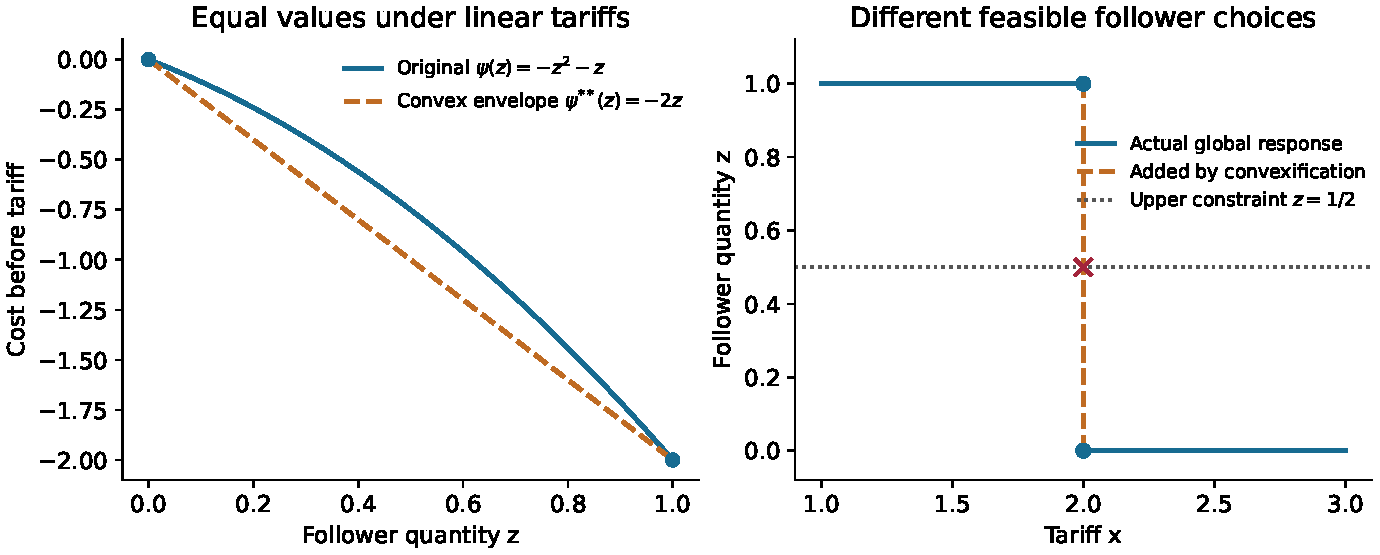
\includegraphics[width=.96\linewidth]{figures/contacts.pdf}
\caption{Example~\ref{ex:false-contacts}. Left: the original aggregate cost and
its convex envelope. Right: original responses retain two contacts at the
switch; the additional vertical segment admitted by convexification consists
of false follower choices.}
\label{fig:contacts}
\end{figure}

Local stationarity is also insufficient: on $[0,1]$,
$f(z)=z/4-z^2/2$ has a strict one-sided local minimum at $0$, of value $0$,
but its global minimum is at $1$, of value $-1/4$. Both points satisfy box KKT.
The examples and the atlas construction therefore treat global selection
explicitly.

\subsection{An independent original-coordinate baseline}
\label{subsec:full-task-baseline}
To compare complete bilevel tasks, we implement a second solver directly in
original coordinates. Enumerating stationary faces of a box quadratic is
classical; see, for example, the discussion in \cite{HladikCernyRada2021}.
The baseline extends this validation to the full price interval and both upper
selection conventions. It shares rational instance data with the compressed
method, but no fiber allocation, envelope construction or upper-optimization
code. It requires that \emph{every principal minor} of
$Q=\diag(d)-huu\trans$ be nonzero: it checks all $2^N-1$ nonempty minors
and rejects an unsupported instance before solving. This restriction excludes
flat follower directions; the compressed method has no such restriction.

\begin{proposition}[Completeness of the original-coordinate baseline]
\label{prop:original-face-baseline}
Under the stated nonzero-principal-minor restriction, enumerating original
stationary box faces, comparing their original objective values over the
whole price interval, and retaining all ties yields the complete response
graph of \eqref{eq:nonconvex-implemented}. The upper tariff problem under both selection conventions, including
attainment, are then solved exactly. Enumeration is exponential in $N$.
\end{proposition}
\begin{proof}
Take any global minimizer and its minimal box face. On its free coordinates
$F$, first-order stationarity holds and the second-order necessary condition
makes $Q_{FF}$ positive semidefinite; its nonzero determinant then makes
it positive definite. Hence this optimizer appears in an enumerated face with
\[
 z_F(x)=-Q_{FF}^{-1}(c_F+\gamma u_Fx+Q_{FB}z_B).
\]
Here $B$ contains both lower and upper fixed coordinates. The baseline
solves this dense original-coordinate system, rejects free faces that are not
positive definite, and intersects the free bounds and bound-gradient signs to
get an exact rational validity interval. A coordinate whose lower and upper
bounds coincide needs no gradient sign. Each retained candidate is feasible,
and every global optimum is retained. Comparing their \emph{original} quadratic
values therefore gives exactly all global optima, regardless of nonglobal KKT
points.

Substitution into $\tfrac12z\trans Qz+(c+\gamma xu)\trans z$ gives a rational
quadratic in $x$. Form all validity endpoints and all pairwise value crossings
on overlaps, including crossings above the global envelope. Exact comparison
on open cells and separately at their endpoints retains all ties. The
nonzero-minor condition rules out a missing continuum: any minimizer in a
positive-dimensional minimal face is the unique stationary point just solved.
Equal winning value polynomials on an open cell have equal derivatives
$\gamma u\trans z$ and hence equal aggregate responses; strict fiber convexity
then makes the entire responses equal.

The baseline independently clips each open response cell with the upper rows
and compares quadratic revenue at endpoints, stationary points and interior
samples, tracking whether each endpoint belongs to the cell. At a cut,
optimistic selection compares all upper-feasible global responses; pessimistic
selection requires all global responses to satisfy the rows and takes their
least revenue. This finite decomposition proves the upper result, including
nonattainment. There are at most $3^N$ faces and quadratically many pair
comparisons in that number; each solve and comparison uses exact rational or
quadratic algebraic arithmetic.
\end{proof}

An earlier independent oracle enumerates original stationary faces at a
single requested price. It may skip singular free faces and still find the
global \emph{value}: a stationary positive-semidefinite singular face has a
null direction along which the quadratic is constant, and moving to the
boundary reduces the face until it is nonsingular or a vertex. This does not
recover a whole flat minimizer set or optimize over all prices; the checked
restriction of the original-coordinate baseline is what makes it a
complete-response and complete-upper-task comparison.

\subsection{Computational protocol and findings}\label{subsec:computations}
All fresh runs use the rational data and deterministic generators in the
accompanying code and data archive, on Linux with an Intel Xeon w5-2565X,
Python 3.13.11, SymPy 1.14.0, NumPy 2.5.1 and SciPy 1.18.0. Each reported
fresh timing is the median of three serial fresh-process runs; all individual
times, wrapper warnings and solver output are retained. OpenBLAS, OpenMP, MKL
and NumExpr were set to one thread, and the SciPy MILP calls also passed
\texttt{threads=1} to HiGHS. Each process starts with the SymPy cache cleared,
and paired methods alternate their order between repetitions to control
shared-cache effects. The machine was shared; we claim no hardware isolation or
statistical speed guarantee. All 60 recorded workers completed within an
external 90-second limit, so no timed-out run is omitted.

The correctness tests compare both global upper outcomes on eight adversarial
and ten seeded small random instances. They compare the entire response sets at
every cut of the baseline's independently constructed face partition and at
an interior sample of each of its cells. For each attained output of \emph{both} methods, they
check bounds, $w=u\trans z$, revenue, every upper row, and the original
follower cost against all valid original-coordinate faces at the returned
price. These returned prices include upper-row boundaries and stationary
revenue points, not just follower switches. Pessimistic witnesses also undergo universal
feasibility and least-revenue checks. Separate tests of the compressed method
cover flat intervals, fixed boxes and singleton aggregates.

Further diagnostics exercise exact convex path certification, forced
numerical-proposal failures, corrupted certificates and missing coverage;
nonconvex original-face value comparisons on signed and fixed-coordinate
instances; and incremental-envelope contacts against a full pairwise partition.
The convex checks include negative rank-one coefficients with positive-definite
total Hessian, nearly singular rational data, and data outside floating-point
range. These finite checks, whose counts are recorded by test family, test
the implementation contracts and specified failure modes; they are not a
formal verification of the general theorems.

\paragraph{The same continuous leader task.}
The heterogeneous family draws $d_i$ uniformly from
$\{8,\ldots,16\}/8$, $u_i$ from $\{4,\ldots,8\}/4$, and $-c_i$ from
$\{4,\ldots,24\}/8$, in that order, with seed $17+N$. It has the unit box,
$x\in[0,5]$, $h=(7/5)/(\sum_i u_i^2/d_i)$, and upper capacity
$u\trans z\le\tfrac12\sum_i u_i$. Its Hessian is indefinite: diagonal
congruence gives $I-hvv\trans$ with $v\trans v=\sum_i u_i^2/d_i$, which has one
negative eigenvalue. Both methods construct the whole response graph and solve the upper problem
under \emph{both} selection conventions with the same upper rows.
Table~\ref{tab:full-task} also includes Example~\ref{ex:capacity-jump}.
Every exact value and attainment flag agrees between the methods and across
repetitions. By total and wall time, the original-coordinate baseline is
faster on the jump and $N=4$ instances, and the compressed method is faster
on the heterogeneous $N=2,6$ instances.
Neither method is uniformly faster, even on these small complete tasks.
The exponential baseline was deliberately limited to $N\le6$, where it checks
at most 63 principal minors and 729 statuses. Larger instances were not
attempted with it, so none is reported as a timeout.

\begin{table}[t]
\centering\small
\caption{Fresh full-task comparisons, seconds (three-run medians).
Faces denotes the original-coordinate baseline; its build includes input
parsing and principal-minor validation. Opt. and pess. solve the upper problem
under the two selection conventions after construction.
Total includes solver input validation, construction and both upper solves;
wall also includes process startup, imports and input-file reading.
Each column is an independently computed median.}
\label{tab:full-task}
\begin{tabular}{llrrrrr}\toprule
$N$ & Method & Build & Opt. & Pess. & Total & Wall\\\midrule
2 (jump) & Compressed & 0.1322 & 0.0102 & 0.0057 & 0.1473 & 0.4348 \\
2 (jump) & Faces & 0.0034 & 0.0007 & 0.0004 & 0.0046 & 0.3018 \\
2 & Compressed & 0.0597 & 0.0014 & 0.0010 & 0.0623 & 0.3541 \\
2 & Faces & 0.1112 & 0.0005 & 0.0004 & 0.1121 & 0.4082 \\
4 & Compressed & 0.6924 & 0.0973 & 0.0665 & 0.8490 & 1.1772 \\
4 & Faces & 0.3334 & 0.2220 & 0.1637 & 0.7074 & 1.0160 \\
6 & Compressed & 0.7014 & 0.2130 & 0.1479 & 1.0605 & 1.3984 \\
6 & Faces & 0.6413 & 0.4266 & 0.3480 & 1.4041 & 1.7100 \\
\bottomrule
\end{tabular}
\end{table}

\paragraph{Symbolic cost and population structure.}
Profiling the unmodified scalar implementation on the $N=12$ heterogeneous
family showed that repeated symbolic cancellation in sign tests dominated the
cost: 5.74 of 9.88 profiled seconds (including instrumentation; not benchmark
times) across the build and one unconstrained upper solve. The copy
distributed with this paper (the \emph{paper copy}) makes two local changes:
it decides the sign of an already
rational expression directly, and it samples the rational midpoint of two
rational interval endpoints. The full exact algebraic fallback and the
candidate, envelope and contact logic are unchanged; the fallback still uses a
rational sample between unrelated quadratic cuts, avoiding unnecessary
output-field extensions.

In ordinary (unprofiled) fresh runs on the same constrained $N=12$ task,
build times were $3.150,2.929,3.107$ seconds for the unmodified
implementation and $2.748,2.679,2.708$ seconds for the paper copy; median
totals including both upper solves were $4.055$ and $3.605$ seconds,
respectively.
This modest improvement supports the two local changes but does not remove the
symbolic cost of heterogeneous events. Table~\ref{tab:scalar-scaling} reports
the remaining fresh scalar runs.

The two-type family has $N=2m$: $m$ copies of $(d,c,u)=(1,-1,1)$ and $m$
copies of $(1,-1/2,1)$, with $h=3/(5m)$, $x\in[0,1]$ and capacity $w\le m$.
Its Hessian is indefinite since $h\sum_i u_i^2/d_i=6/5$.
Uniqueness of the local fiber allocation makes coordinates within each type
equal. Dividing costs and aggregate by $m$ reduces the response problem exactly
to Example~\ref{ex:capacity-jump}. Therefore the optimistic optimum is
$51m/160$ at price $17/20$ and aggregate $3m/8$, while the pessimistic
supremum is the same and is not attained. There are three fiber pieces and seven
atlas points for every $m$. The $N=1000$ run thus tests repeated types, whereas
$N=48$ has 66 fiber pieces; their timings measure different structural regimes.

\begin{table}[t]
\centering\small
\caption{Fresh compressed scalar runs, seconds (three-run medians).
The last two upper columns concern the same capacity row. Total includes input
validation, build and both upper solves; process wall times and all repetitions
are in the data archive.}
\label{tab:scalar-scaling}
\begin{tabular}{lrrrrrr}\toprule
$N$ & Fiber pieces & Atlas points & Build & Opt. & Pess. & Total\\\midrule
12 & 21 & 45 & 2.7076 & 0.4769 & 0.4346 & 3.6053 \\
24 & 38 & 79 & 3.9774 & 0.8773 & 0.7808 & 5.6096 \\
48 & 66 & 135 & 13.6697 & 2.7917 & 2.8244 & 19.2916 \\
20 (two types) & 3 & 7 & 0.1365 & 0.0413 & 0.0331 & 0.2039 \\
200 (two types) & 3 & 7 & 0.1415 & 0.2125 & 0.2828 & 0.6275 \\
1000 (two types) & 3 & 7 & 0.2388 & 1.2650 & 1.6078 & 3.1009 \\
\bottomrule
\end{tabular}
\end{table}

The separate convex tariff family uses $u_i=1$, $h=1/(10N)$,
$d_i\in\{5,\ldots,20\}/10$, $-c_i\in\{1000,\ldots,25000\}/10000$,
$x\in[0,3]$, a service floor $\sum_i z_i\ge N/5$, and seeds $50001+N$.
The fused aligned sweep and upper solve had fresh median times of
$0.014$, $0.117$ and $1.100$ seconds for $N=100,1000,10000$, respectively;
input generation and validation added $0.0005$, $0.0032$ and $0.0336$ seconds.
Every returned response passed exact KKT and service-floor checks. These
synthetic convex results do not measure the nonconvex atlas or a general
large-scale bilevel model.

Earlier archived runs used different cache and repetition protocols, so
their differences from fresh timings are not controlled speedup estimates.
The older all-pair compressed implementation, a different comparator from the
original-coordinate baseline, kept 274 atlas points for $N=12$, compared with
45 after incremental envelope insertion; its recorded build medians were
$15.882$ and $3.079$ seconds. Archived timings were $18.699$ seconds for
construction and $2.922$ for one upper solve at heterogeneous $N=48$, $0.255$
and $1.261$ seconds at two-type $N=1000$ (three fiber pieces, seven atlas
points), and $1.047$ seconds for the convex $N=10000$ fused sweep. The earlier
generic convex-path runs retain their exact certificates and small dense-KKT
MILP comparisons; they support the certificate interface but do not guarantee
completeness of numerical proposals on arbitrary inputs.

\paragraph{Dense screening: a negative timing result.}\label{para:screening-results}
The exact screening prototype implements certified dense screening, in the
scalar-cell specialization of
Section~\ref{sec:robust-screening}. The identity surrogate has a diagonal
response cover; the true dense Hessian is a rational symmetric perturbation
with verified strict diagonal dominance. Screening fixes certified statuses,
and exact original KKT recovery enumerates the ambiguous ones. The bound
$M3^t$ counts recovery LPs only; dense inversion, cover construction and
certification are additional real computational costs.

The independent numerical comparator uses two binary variables $l_i,u_i$ per
coordinate and $g=Qz+c+Cx$, imposing
\[
 z_i+l_i\le1,\quad z_i-u_i\ge0,\quad l_i+u_i\le1,
 \qquad -M_i u_i\le g_i\le M_i l_i,
\]
with $0\le z_i\le1$ and
$M_i=1+|c_i|+|C_i|\max(|L|,|R|)+\sum_j|Q_{ij}|$.
If both binaries vanish, $g_i=0$; if $l_i=1$ or $u_i=1$, the corresponding
bound and gradient sign hold. Conversely, every box KKT point admits such
binaries, including zero-gradient bounds. By positive definiteness this is an
exact reformulation in real arithmetic. Its SciPy--HiGHS solve is numerical,
with a 30-second limit and requested relative MIP gap zero; numerical primal
and dual reports are not rational optimality certificates.

\begin{table}[t]
\centering\small
\caption{Screening versus dense KKT MILP, seconds. Archived entries are single
runs; fresh entries are three-run medians. Exact preprocessing includes input
generation and surrogate cover; exact total also includes final rational
verification. MILP preprocessing includes input generation and formulation.
Tighter-tolerance follow-ups are excluded from the default-solve columns.}
\label{tab:screening-negative}
\begin{tabular}{llrrrrrr}\toprule
 & &\multicolumn{3}{c}{Exact screening}&\multicolumn{3}{c}{Numerical MILP}\\
Source&$N$&Preprocess&Solve&Total&Preprocess&Solve&Total\\\midrule
Archived & 8 & 0.0034 & 0.0984 & 0.1023 & 0.0023 & 0.0243 & 0.0265 \\
Archived & 12 & 0.0141 & 0.2962 & 0.3112 & 0.0045 & 0.0382 & 0.0427 \\
Archived & 20 & 0.0142 & 0.9332 & 0.9509 & 0.0078 & 0.1560 & 0.1638 \\
Archived & 40 & 0.0334 & 17.5689 & 17.6121 & 0.0256 & 0.4041 & 0.4297 \\
Fresh & 8 & 0.0046 & 0.1273 & 0.1335 & 0.0025 & 0.0180 & 0.0203 \\
Fresh & 20 & 0.0200 & 0.9056 & 0.9293 & 0.0084 & 0.1624 & 0.1699 \\
\bottomrule
\end{tabular}
\end{table}

The exact prototype was slower on all four archived instances, and the fresh
$N=8,20$ repetitions confirm this after including preprocessing
(Table~\ref{tab:screening-negative}). Their maximum ambiguity is two, with
105 and 285 completed cell/status assignments. The archived $N=40$ case has
maximum ambiguity four and 2304 completed assignments; rational recovery alone
took $15.29$ of $17.57$ solver seconds.

The default $N=8$ MILP reports optimality and zero gap but an objective
$3.3703\cdot10^{-7}$ below the exact value
$4810519997/235205877942$, with a modeled-row violation of approximately
$3.5387\cdot10^{-7}$. This discrepancy occurs in the archived run and in
all fresh repetitions. With primal and MIP feasibility tolerances
$10^{-9}$, the objective agrees within $3.82\cdot10^{-17}$ and the maximum
row violation is $1.11\cdot10^{-16}$. At $N=20$, agreement is within $1.34\cdot10^{-15}$. The returned
exact screening solutions satisfy all rows and dense KKT equations rationally;
their global guarantee rests on the screening theorem, not on checking a
returned point alone.

The supplement preserves the rational instances, generator seeds, input
hashes, software and machine metadata, individual timings and exact diagnostic
logs. The experiments establish reproducible behavior for the stated scalar
subclasses only. They do not implement the general quantifier-elimination
algorithms and give no evidence of superiority on industrial instances or
arbitrary heterogeneous follower populations.

\section{Conclusions}\label{sec:conclusions}

The positive results are controlled by the dimension needed to describe
follower responses after local elimination. For quadratic blocks, positive
local curvature gives rational response formulas, and a fixed number of
shared multipliers and aggregates bounds the number of joint regimes.
Comparing actual follower values in this compressed space makes the
description global even for a nonconvex aggregate cost. The description
supports polynomial upper data, both selection conventions and explicit
attainment decisions. For near-optimal responses, fixing the measurements
of each criterion separately gives the corresponding reduction without
assuming that admissible followers are stationary.

For higher-degree local costs, arithmetic output becomes part of the
problem: a large algebraic field can be unavoidable even for independent,
uniformly convex scalar followers. Uniform rational inverse approximations
allow global upper optimization without forming that field, with a bound
polynomial in accuracy bits for the fixed dimensions and numerical degrees.
The rational output is exactly feasible for the base leader polytope.
Response-dependent upper feasibility needs a separate argument: relaxed
upper rows, an inner certificate and an original-feasibility decision
cannot be interchanged. The sharp $1/P$ response modulus and the stated
margin conditions make these distinctions quantitative.

The boundary results show that numerical simplicity and graph sparsity
cannot replace these hypotheses. A dense follower Hessian arbitrarily close
to the identity still admits an exact hardness reduction; this is
compatible with a condition-dependent scheme polynomial in inverse
normalized error. A path can have exponentially many response pieces or
elimination segments yet admit inexpensive pointwise evaluation. Hardness
of an upper problem, the size of an explicit response representation and
the cost of one follower solve are therefore separate questions. The
positive bounded-core and equal-gain projection results require their full
stated assumptions; neither implies tractability of unrestricted paths.

The scalar implementations make the response-set requirement concrete.
Convexification preserves every tilted follower value, but an original
contact test is necessary to prevent false upper feasibility. The
independent original-coordinate baseline agrees with the compressed method on
both complete upper tasks for the tested small instances. Larger
computations separate heterogeneous events from repeated coordinate types.
In the dense screening experiments, even small certified ambiguity did not
compensate for exact preprocessing and recovery costs against the tested
numerical MILP comparator. The computations support the specified
algorithms and certificates; the general complexity results rest on their
proofs.

\paragraph{Code and data.}
The computational supplement contains the scalar implementations, the
independent baseline, exact diagnostics, rational instance data, individual
run records and the scripts that generate the reported tables and figure.
Its README gives reproduction commands, dependencies and the provenance of
historical measurements and later corrections. The mathematical arguments
and the LaTeX build do not depend on the supplement.

\appendix
\section{Polyhedral blocks coupled through a fixed core}\label{app:fixed-core}

This appendix proves a related elimination theorem for a single-level
problem that is linear in many small polyhedral blocks and polynomial in
a fixed-dimensional core. It gives a broader structural comparison and
makes witness recovery explicit. Its convex combinations preserve
polyhedral feasibility and linear measurements; they are not combinations
of globally optimal responses of a nonconvex follower.

Fix $r,k\ge0$ and $d\ge1$. Let $C\subset\R^r$ be compact and given by an explicit
rational quantifier-free polynomial formula. For $b=1,\ldots,B$, let
\[
 P_b(x)=\{y\in\R^{d_b}:G_b(x)y\le h_b(x)\},\qquad 1\le d_b\le d,
\]
with polynomial rational data and explicit finite rational coordinate
bounds among its rows. The local sets may be empty or lower-dimensional.
Let $A_b(x)\in\Q[x]^{k\times d_b}$, $b(x)\in\Q[x]^k$,
$c_b(x)\in\Q[x]^{d_b}$ and $c_0(x)\in\Q[x]$. Consider
\begin{equation}\label{eq:fixed-core-problem}
 \begin{aligned}
 \min_{x,z}\quad&c_0(x)+\sum_{b=1}^B c_b(x)\trans z_b,\\
 \text{subject to}\quad&x\in C,\quad z_b\in P_b(x)\quad(b=1,\ldots,B),\\
 &\sum_{b=1}^B A_b(x)z_b=b(x).
 \end{aligned}
\end{equation}
Let $L$ be the input length, including all explicit data, and let
$\delta\ge2$ bound the actual input degree. The theorem tracks the
numerical degree throughout instead of fixing it.

\begin{theorem}[Fixed-core polyhedral optimization]\label{thm:fixed-core}
For fixed $r,d,k$, feasibility and global optimization of
\eqref{eq:fixed-core-problem} are computable in time polynomial in
$(L,\delta)$. If feasible, an optimum is attained and an optimizer with
all block coordinates and its value can be returned in a single
real-algebraic field with polynomial total encoding length. Neither the
number of blocks nor their row counts is fixed. A fixed number of
aggregate inequalities is also allowed if finite bounds for their
slacks are supplied.
\end{theorem}

\subsection{Local vertices and support directions}\label{app:local-support}

For block $b$ enumerate all $d_b$-row subsets $I$. Put
\[
 \Delta_{bI}(x)=\det (G_b(x))_I,\qquad
 p_{bI}(x)=\operatorname{adj}((G_b(x))_I)(h_b(x))_I.
\]
Where $\Delta_{bI}\ne0$, the candidate is
$p_{bI}/\Delta_{bI}$. Equivalently, use the positive-denominator form
\begin{equation}\label{eq:core-vertex-formula}
 D_{bI}=\Delta_{bI}^2,\qquad Y_{bI}=\Delta_{bI}p_{bI},\qquad
                          y_{bI}=Y_{bI}/D_{bI}.
\end{equation}
Its validity predicate is
\begin{equation}\label{eq:core-vertex-validity}
 D_{bI}>0,\qquad G_b(x)Y_{bI}(x)\le h_b(x)D_{bI}(x).
\end{equation}
All these tests are polynomial of degree $O(d\delta)$.

Every vertex of $P_b(x)$ has $d_b$ independent active rows. Otherwise
some nonzero direction is orthogonal to all active normals; a small
step in either direction keeps the active rows tight and preserves the
finitely many strict inactive rows, contradicting extremality. A
nonempty bounded polyhedron has a vertex, and every linear functional
has a maximizing vertex: a maximizing face is nonempty and compact, and
successively minimizing the coordinates within it produces a singleton
face, which is a vertex of the original polyhedron. These arguments also
apply to lower-dimensional sets and singletons. Thus
\eqref{eq:core-vertex-formula} lists enough candidates to detect
nonemptiness and maximize every linear functional.

Append the objective as a measurement. With $h=k+1$, define
\begin{equation}\label{eq:core-images}
 W_b(x)=\begin{pmatrix}A_b(x)\\c_b(x)\trans\end{pmatrix},\quad
 T_b(x)=W_b(x)P_b(x),\quad
 t(x,\eta)=\begin{pmatrix}b(x)\\\eta-c_0(x)\end{pmatrix}.
\end{equation}
For a direction $\lambda\in\R^h$, the support score of a valid
vertex is
\[
 \lambda\trans W_b(x)y_{bI}(x)=n_{bI}(x,\lambda)/D_{bI}(x),\qquad
 n_{bI}=\lambda\trans W_bY_{bI}.
\]
Collect the denominator and validity polynomials, and, for every pair
of candidates in one block, the comparison polynomial
\begin{equation}\label{eq:core-score-comparison}
                     n_{bI}D_{bJ}-n_{bJ}D_{bI}.
\end{equation}
Valid candidates have positive denominators, so these signs order their
scores correctly. For fixed $d$ there are polynomially many such
polynomials, all in the $r+h$ coordinates $(x,\lambda)$, of degree
$O(d\delta)$ and polynomial coefficient bit length.

Enumerate their realizable sign conditions, including zero signs and
recording identically zero polynomials. Each sign condition determines the
valid vertices of every block and, for every nonempty block, a
support-maximizing vertex; choose the first maximizer in a fixed ordering.
Discard a condition if some block has no valid candidate. For fixed
$(r,d,k)$, the retained list $\Sigma$ has polynomial size and can be
constructed in polynomial bit time. Disconnected sign realizations cause no
problem, since signs alone determine validity and score order.

\subsection{Exact membership from the support inequalities}\label{app:support-membership}

For $\sigma\in\Sigma$, let $I_b(\sigma)$ be its selected local
index and abbreviate the corresponding denominator and numerator by
$D_{b\sigma},n_{b\sigma}$. Put
\begin{equation}\label{eq:core-cleared-support}
 \begin{split}
 H_\sigma(x)&=\prod_bD_{b\sigma}(x),\\
 J_\sigma(x,\eta,\lambda)&=
 \lambda\trans t(x,\eta)H_\sigma(x)
             -\sum_b n_{b\sigma}(x,\lambda)\prod_{a\ne b}D_{a\sigma}(x).
 \end{split}
\end{equation}
On that sign condition $H_\sigma>0$, and $J_\sigma\le0$ states the
support inequality
\[
 \lambda\trans t(x,\eta)\le
                     \sum_b\max_{y\in P_b(x)}\lambda\trans W_b(x)y.
\]
Writing $S_\sigma(x,\lambda)$ for the sign conjunction, define
\begin{equation}\label{eq:core-support-predicate}
 \Phi(x,\eta,\lambda)=\bigvee_{\sigma\in\Sigma}
                  [S_\sigma(x,\lambda)\wedge J_\sigma(x,\eta,\lambda)\le0].
\end{equation}

\begin{lemma}[Support membership]\label{lem:core-support-membership}
For $x\in C$, there exist blocks satisfying
\eqref{eq:fixed-core-problem} with objective exactly $\eta$ if and only if
\begin{equation}\label{eq:core-membership}
                           \forall\lambda\in\R^h\ \Phi(x,\eta,\lambda).
\end{equation}
\end{lemma}
\begin{proof}
If a block is empty, then for every $\lambda$ no retained sign condition
is realized at $(x,\lambda)$, so \eqref{eq:core-membership} is false.
Otherwise the Minkowski sum
$T(x)=\sum_bT_b(x)=\{\sum_b t_b:t_b\in T_b(x)\}$ is compact and
convex. Its support function is the sum of the support functions of its
summands, since a maximizer can be chosen independently in every block.
Hence \eqref{eq:core-support-predicate} gives its exact support
inequality in every direction.

A point $t$ in a compact convex set $T$ satisfies all its support
inequalities. Conversely, if $t\notin T$, choose a nearest point
$p\in T$ and put $\lambda=t-p\ne0$. The derivative of squared
distance along the segment from $p$ to any $u\in T$ gives
$(t-p)\trans(u-p)\le0$. Hence
$\max_{u\in T}\lambda\trans u\le\lambda\trans p
<\lambda\trans t$, violating a support inequality.
Thus \eqref{eq:core-membership} is equivalent to $t(x,\eta)\in T(x)$.
By \eqref{eq:core-images}, this membership states precisely existence
of blocks satisfying all linking equations and attaining the specified
objective value.
\end{proof}

The degrees in \eqref{eq:core-cleared-support} are
$O((B+1)d\delta)$, which need not be constant. Their ambient dimension
$r+h+1$ is fixed, however, so by the product argument in
\cref{lem:candidate-size} their expanded monomial count and bit size
are polynomial in $(L,\delta)$. Define
\[
 E(x,\eta)=(x\in C)\wedge\forall\lambda\,\Phi(x,\eta,\lambda).
\]
This formula in a fixed number of variables describes exactly the
attainable core--value pairs. The feasible set of
\eqref{eq:fixed-core-problem} is closed and lies in the product of the
compact set $C$ and the finite block boxes, so the minimum is attained
whenever the problem is feasible. Apply quantifier elimination and joint
sampling to
\begin{equation}\label{eq:core-joint-optimum}
 E(x,\eta)\wedge
       \neg\exists x',\eta'\,[E(x',\eta')\wedge\eta'<\eta].
\end{equation}
This gives an optimal $(x^*,\eta^*)$ in one field
$K=\Q(\alpha)$ of polynomial degree and encoding length.
It remains to recover all block variables. Making each of them a
quantified coordinate would destroy the fixed-dimensional argument.

\subsection{Constructive recovery from a few support tuples}\label{app:core-recovery}

The support enumeration already supplies a polynomial-size set of
full block tuples that suffices for recovery. For each $\sigma\in\Sigma$,
evaluate its selected local denominators at $x^*$ and discard the tuple
if any is zero. Otherwise evaluate the vertex formulas and retain the
tuple if every selected local vertex is feasible at $x^*$. Denote the
retained tuples by $y^1,\ldots,y^M$, and set
\[
              a^j=\sum_b W_b(x^*)y_b^j\in K^h\qquad(j=1,\ldots,M).
\]
The filter does not require the sign condition $\sigma$ to be realizable
at $x^*$ with some direction: feasibility of the tuple suffices, and the filter
never adds a point outside $T(x^*)$.

\begin{lemma}[A small common convex combination recovers every block]
\label{lem:core-recovery}
The retained aggregate points satisfy
$\conv\{a^1,\ldots,a^M\}=T(x^*)$. For every target $t\in K^h\cap T(x^*)$
one can find at most $h+1$ retained tuples and nonnegative weights in $K$
that sum to one and whose weighted aggregate is $t$, in polynomial bit
time in the original input and target encoding. Using the same weights
in every block gives a feasible original tuple with aggregate $t$.
\end{lemma}
\begin{proof}
Every retained tuple is blockwise feasible, so its aggregate belongs to
$T(x^*)$ and the indicated convex hull is contained in $T(x^*)$.
For every real direction $\lambda$, the actual sign condition at
$(x^*,\lambda)$ is retained in $\Sigma$: no block is empty at an
optimal core. Its selected vertices give a feasible tuple that attains
the support of $T(x^*)$ in direction $\lambda$. This tuple survives
the filter. Hence the convex hull has the same support function as
$T(x^*)$. The separation argument in \cref{lem:core-support-membership}
proves equality.

The usual Carath\'eodory reduction gives a convex representation of
a target in a finite convex hull with affinely independent support.
To see this directly, start with a representation whose weights on its
support are all positive. If its lifted
columns $(a^j,1)$ are dependent, choose a nonzero dependence $u$.
Its components sum to zero, so it has a positive component. Replace
the weights $\theta_j$ by $\theta_j-su_j$, with
$s=\min_{u_j>0}\theta_j/u_j$. This preserves the target and the sum
of weights, keeps weights nonnegative, and removes at least one support
point. Repeat until the lifted columns are independent. Their number
is at most $h+1$.

For construction, enumerate all subsets of at most $h+1$ retained
points. On each affinely independent subset solve
\[
          \sum_j\theta_j a^j=t,\qquad \sum_j\theta_j=1.
\]
Choose independent rows to solve this fixed-size system, then check
all remaining equations and the nonnegativity of its unique weights.
If a suitable subset exists over the reals, the unique solution of its
independent linear system lies in $K$, since every coefficient and the
target belong to $K$. Thus the enumeration finds it. There are at most
$\sum_{q=1}^{h+1}\binom Mq$ subsets, polynomial for fixed $h$.
All arithmetic, zero tests, and comparisons take place in the already
sampled ordered field $K$, whose degree and coefficient encodings are
polynomial. Each system has fixed order, so determinant expressions
and rational evaluation give polynomial coefficient lengths for the
weights; summing the resulting fixed number of terms preserves the
same bound for every recovered block coordinate.

Finally, put $z_b=\sum_j\theta_j y_b^j$ for every block. Convexity
of $P_b(x^*)$ makes $z_b$ feasible, and linearity of $W_b(x^*)$ gives
$\sum_bW_b(x^*)z_b=t$. The same weights must be used in all blocks:
this is how the prescribed total measurements are preserved.
\end{proof}

Applying \cref{lem:core-recovery} to
$t=t(x^*,\eta^*)$ recovers the original optimizer in the field $K$,
which proves the main claim of \cref{thm:fixed-core}. With no blocks,
the image sum is $\{0\}$ and the empty tuple is its only support tuple;
empty sums and products have their usual meanings. Blocks of dimension
zero can be removed after testing their scalar rows. A fixed number of
aggregate inequalities become equalities with bounded scalar slack
blocks; the supplied slack bounds keep the model compact and do not
change the fixed structural dimensions.

The running time is polynomial in the numerical input degree as well as
the input length: local determinants and pair comparisons have degree
$O(d\delta)$; the global products have degree $O((B+1)d\delta)$; sign
enumeration, elimination and sampling are all in fixed dimension; and
reconstruction adds only fixed-size algebraic linear systems. Under
polynomially bounded degree, the time is polynomial in $L$.

The common support-direction construction has a direct predecessor in
Gritzmann and Sturmfels~\cite[Algorithm 2.3.6, Theorem 2.3.7, and
Corollary 2.3.10]{GritzmannSturmfels1993}: for fixed-dimensional input
polytopes, they enumerate a shared arrangement of support directions and
compatible maximizing summand vertices, with polynomial binary complexity.
Beyond that construction, we prove that the sign enumeration is uniform
over the polynomially varying core, and that exact optimization and
reconstruction recover all original blocks in one common field. The
support characterization, finite-dimensional convex-hull reduction and
real algebraic algorithms are established tools. An alternative recovery
would solve a linear program over the sampled common field; Adler and
Beling~\cite{AdlerBeling1994} analyze that route with explicit dependence
on the common extension degree. The recovery above instead reuses the
support tuples already generated and needs no large-dimensional algebraic
LP solve. It relies on the affine block measurements, including the
objective coordinate, and would not justify convexifying a nonconvex
follower response set or mixing its tied responses to create additional
follower choices.

\section{Uniform rational approximation of polynomial inverses}
\label{app:inverse}

This appendix proves the approximation interface used in
\cref{sec:accuracy}. Polynomial inverse approximation and algebraic-series
computation have established algorithms
\cite{Farouki2000,Walsh2000}. The purpose here is to give the complete
uniform error and rational encoding bounds, including flat points of a
strictly increasing marginal. The analytic ingredients are the classical
holomorphic inverse, Cauchy estimates, and Rouch\'e theorem
\cite{DLMFComplex}.

\begin{lemma}[Effective increment and inverse bounds]\label{lem:inverse-modulus}
Let $g\in\Q[t]$ have degree $D\ge1$, be strictly increasing on $[0,1]$,
and satisfy $g(0)=0$, $g(1)=1$. For $[a,a+h]\subseteq[0,1]$,
\begin{equation}\label{eq:inverse-increment}
             g(a+h)-g(a)\ge\frac12\left(\frac{h}{2D}\right)^D.
\end{equation}
Consequently the clipped inverse changes by less than $e$ whenever its
argument changes by less than $\frac12(e/(2D))^D$, for $0<e\le1$.
For an unnormalized marginal with endpoint difference $G>0$, multiply
this argument tolerance by $G$.
\end{lemma}
\begin{proof}
For $h>0$ put $v=g(a+h)-g(a)$. Interpolate $g-g(a)$ at
$a+jh/D$, $j=0,\ldots,D$. All node values lie in $[0,v]$.
On $[0,1]$ every factor in the numerator of a Lagrange basis polynomial
has absolute value at most one, and its denominator has magnitude
$(h/D)^D j!(D-j)!$. Thus
\[
 |g(t)-g(a)|\le v(D/h)^D\sum_{j=0}^D\frac1{j!(D-j)!}
              \le v(2D/h)^D.
\]
Applying this at $t=0,1$ gives $1\le2v(2D/h)^D$. The case $h=0$
is immediate. An inverse displacement of at least $e$ contains a
response interval of length $e$, so requires at least the displayed
argument displacement. If clipping occurs, the argument interval only
gets longer. Positive affine normalization proves the last assertion.
\end{proof}

\begin{theorem}[Rational inverse approximation]\label{thm:inverse-approximation}
For a densely encoded rational polynomial $g$ strictly increasing on
$[0,1]$, and a positive rational tolerance $\eta$, one can construct
rational breakpoints and rational polynomial branches approximating its
clipped inverse uniformly to error $\eta$. Each branch is valid on its
closed interval, with constant branches outside $[g(0),g(1)]$.
Construction time, number of branches, degrees, and rational encoding
lengths are polynomial in input bits, numerical degree, and
$\max\{0,\log(1/\eta)\}$. The encoding of $\eta$ is part of the input;
equivalently one can request $\eta=2^{-B}$ at cost polynomial in $B$.
No positive lower bound on $g'$ is required.
\end{theorem}
\begin{proof}
Normalize to $g(0)=0,g(1)=1$ by a rational affine change of target.
Replace $\eta$ by $\min\{\eta,1/2\}$, and put
\begin{equation}\label{eq:inverse-bad-tolerance}
 e=\eta/4,\qquad \delta_0=\tfrac14(e/(2D))^D,\qquad
 \rho=\text{largest dyadic number at most }
          \min\{\delta_0/[4(D+1)],1/16\}.
\end{equation}
Their bit lengths are polynomial in the stated parameters. An interval
of target length at most $\delta_0$ has inverse oscillation less than
$e$, by \cref{lem:inverse-modulus}.

\emph{Critical values, including nonreal ones.}
The real parts of all finite complex critical values are the real $s$
satisfying
\begin{equation}\label{eq:critical-projection}
 \exists u,v:\quad
 \Re g'(u+\mathrm i v)=\Im g'(u+\mathrm i v)=0,\qquad
                         s=\Re g(u+\mathrm i v).
\end{equation}
The formula has three real variables and polynomials of degree at most
$D$ with polynomial-size dense expansions. Fixed-dimensional elimination
and univariate isolation from \cref{subsec:tools} compute this finite
set, of cardinality at most $D-1$, in polynomial bit time. For $D=1$ it
is empty. Repeated critical points or coincident real parts cause no
problem. Keeping only real critical values would be insufficient for the
analytic argument below.

Retain the real parts in $[-1,2]$, bracket each in a rational interval
of width at most $\rho$, and pad that interval by $\rho$ at both ends.
Add $[-\rho,\rho]$ and $[1-\rho,1+\rho]$, intersect the union with
$[0,1]$, and merge overlapping intervals. Denote the result by $B_0$.
The sum of untrimmed lengths is at most
$3(D-1)\rho+4\rho\le\delta_0$. Each merged component therefore has
length at most $\delta_0$. On it use a constant rational approximation,
within $e$, to the inverse at its rational midpoint. Monotone bisection
in response space computes that constant in polynomial time. Its error
on the entire component is less than $2e$. This also treats endpoints
and interior derivative zeros.

For a complementary gap $[a,b]$, define
\[
                    d(t)=\min\{t-a+\rho,b-t+\rho\}.
\]
Every critical real part is at distance at least $d(t)$ from $t$.
For retained parts, padding places them at least $\rho$ behind the
exposed endpoint of their merged component. Omitted parts lie outside
$[-1,2]$, at distance greater than one, whereas
$d(t)\le1/2+\rho<1$.

\emph{Rational analytic panels.}
Split each gap at $m=(a+b)/2$. Starting at $x=a$, set
\[
                  y=\min\{m,x+(x-a+\rho)/32\}
\]
and take $[x,y]$ as the next panel; reflect this construction on the
right half. Before the final panel, $x-a+\rho$ grows by $33/32$.
Thus each gap has $O(1+\log(1/\rho))$ panels, all with polynomial
rational bit length. There are at most $D+1$ gaps. At a panel midpoint
$\tau$, put $d=d(\tau)$; the panel half-width is at most $d/64$.

Writing $g(z)=\sum a_jz^j$, the rational number
$L_g=\max\{1,\sum j|a_j|\}$ bounds $g'$ in absolute value on
$[0,1]$. Bisection of the inverse bracket to width $d/(64L_g)$
provides a rational midpoint $z_0\in(0,1)$ such that
$|g(z_0)-\tau|\le d/64$. Set $t_0=g(z_0)$ and $R=d/4$.
Every complex critical value has distance at least $63d/64$ from
$t_0$. Hence a neighborhood of the closed radius-$R$ disk contains
no critical value. Every panel target satisfies
\begin{equation}\label{eq:inverse-panel-ratio}
                       |t-t_0|\le d/32\le R/8.
\end{equation}

For completeness, the inverse branch exists on that entire disk, not
merely on its real diameter. A polynomial is proper: the modulus of its
leading term forces $|g(z)|\to\infty$ as $|z|\to\infty$.
Away from critical values each preimage is simple, and the local
holomorphic inverse theorem gives disjoint inverse neighborhoods for
its finitely many roots. Properness ensures that these neighborhoods
exhaust preimages after shrinking the target neighborhood; otherwise a
sequence of additional preimages has a bounded convergent subsequence,
contradicting local uniqueness. Thus the restriction is a finite
covering. Path lifting over the simply connected disk gives one inverse
on each connected component, with no monodromy. It is holomorphic by
local inversion. Select the component through $z_0$. Along the real
segment to every panel target this branch equals the real increasing
inverse by uniqueness and continuity. In particular $g'(z_0)\ne0$.

\emph{Taylor approximation and rational arithmetic.}
On the disk $|t|<2$. The elementary polynomial root bound gives
\[
 |Z(t)|\le M_g:=2+\frac{2+\sum_{j<D}|a_j|}{|a_D|}.
\]
Indeed, a root of $a_Dz^D+\sum_{j<D}\widetilde a_jz^j$ has
modulus at most $1+\max_{j<D}|\widetilde a_j/a_D|$, and the
constant coefficient changes by less than two. Cauchy's estimate for
$Z(t_0+v)=z_0+\sum_{n\ge1}c_nv^n$ yields
$|c_n|\le M_gR^{-n}$. With
$q\ge\lceil\log_2(4M_g/\eta)\rceil$, the tail on the panel is
at most $M_g2^{-q}\le\eta/4$, using the weaker ratio $1/2$ in
\eqref{eq:inverse-panel-ratio}.

All coefficients are rational, since the expansion center is a
\emph{rational response} rather than an approximate irrational inverse.
Write
\[
 g(z_0+u)-t_0=Q^{-1}\sum_{h=1}^D A_hu^h,
 \qquad Q\in\Z_{>0},\ A_h\in\Z,\ A_1\ne0.
\]
Formal substitution gives
\begin{equation}\label{eq:inverse-reversion}
 \begin{split}
 c_1&=Q/A_1,\\
 c_n&=-\frac1{A_1}\sum_{h=2}^{\min(D,n)}A_h[v^n]
                       \left(\sum_{j=1}^{n-1}c_jv^j\right)^h.
 \end{split}
\end{equation}
A factor containing $c_n$ cannot contribute to degree $n$ in a power
$h\ge2$, which proves the triangular recurrence. Inductively
\begin{equation}\label{eq:inverse-denominator}
                    c_n=Q^nN_n/A_1^{2n-1},\qquad N_n\in\Z.
\end{equation}
A product of $h$ earlier coefficients with indices summing to $n$
has denominator $A_1^{2n-h}$ after factoring $Q^n$. The additional
division by $A_1$ and conversion to the displayed denominator multiplies
its integer numerator by $A_1^{h-2}$. Signs are irrelevant.

Translation of $g$ to $z_0$ has polynomial encoding; so do $Q,A_h$.
The denominator in \eqref{eq:inverse-denominator} and Cauchy's magnitude
bound give polynomial numerator and denominator bit lengths, because
$q$, $\log M_g$, and $\log(1/R)$ are polynomially bounded. The same
holds for intermediate truncated convolutions: each term has at most
$q$ earlier factors, and at most $2^{q-1}$ compositions contribute to
any fixed degree before the polynomially many sums over $h$.
Using these common denominators keeps all arithmetic polynomial in bit
cost. Truncated polynomial multiplication uses polynomially many
operations, without enumerating the compositions. Ordinary-power
expansion of the Taylor polynomials preserves the bounds.

The constant pieces on $B_0$, Taylor pieces on the gaps, and exact
clipped constants cover the line. Adjacent branches each satisfy the
error bound at their shared endpoint; they need not agree exactly.
A half-open convention defines a single approximating function if needed.
Undoing the target normalization proves the theorem.
\end{proof}

\begin{proposition}[Sharper positive-coefficient construction]
\label{prop:positive-inverse}
If $g(z)=\sum_{j=1}^P a_jz^j$ with $a_j\ge0$ and $g(1)>0$,
the approximation in \cref{thm:inverse-approximation} can use
$O(P^2\log(1/\eta))$ nonconstant branches, each of degree
$O(\log(1/\eta))$, independently of coefficient conditioning in these
two counts. Coefficient bit lengths still depend polynomially on the
input encoding. Numerical, rather than sparsely encoded binary, $P$
is the complexity parameter.
\end{proposition}
\begin{proof}
Normalize $g(1)=1$. Termwise,
\[
 z^P\le g(z)\le z,\quad 0\le g'(z)\le P,\quad
                g(z)\le zg'(z)\le Pg(z)\quad(0<z\le1).
\]
Take $m=\lceil\log_2(1/\eta)\rceil\ge1$ after reducing
$\eta$ to at most $1/2$, and $K_0=Pm$. Below $2^{-K_0}$ the
constant zero has error at most $2^{-m}$; above one use the exact
constant one.

For real $0<z_0\le1$, put $t_0=g(z_0)$,
$r_z=z_0/(4P)$ and $R_t=t_0/(8P)$. Nonnegative coefficients give,
for complex $|u|\le r_z$,
\[
 |g'(z_0+u)-g'(z_0)|
 \le g'(z_0)((1+1/(4P))^{P-1}-1)<g'(z_0)/3.
\]
Here $e^{1/4}<4/3$ follows by termwise comparison with a geometric
series. Integrating along the segment gives
\[
 |g(z_0+u)-t_0-g'(z_0)u|\le g'(z_0)|u|/3.
\]
On $|u|=r_z$, the shift $|t-t_0|\le R_t$ is at most
$g'(z_0)r_z/2$. The nonlinear remainder plus shift is therefore
at most $5/6$ of the linear comparison magnitude. Rouch\'e gives
exactly one root in the response disk; the derivative bound makes it
simple. Local inverses agree by uniqueness, and the strict boundary
margin extends them to a neighborhood of the closed target disk.
The resulting branch satisfies $|Z(t)|<2$ and agrees with the
positive real inverse on real targets in $[0,1]$.

Split each dyadic interval $[A,2A]$, $A=2^{-(k+1)}$,
$k=0,\ldots,K_0-1$, into $32P$ equal rational panels. At midpoint
$\tau$ the panel half-width is at most $\tau/(64P)$.
Bisection to response width $\tau/(64P^2)$ produces rational
$z_0$ with $|t_0-\tau|\le\tau/(64P)$ and
$t_0\ge63\tau/64$. Thus on its panel
\[
             |t-t_0|/R_t\le16/63<1/2.
\]
The bisection takes $K_0+O(\log P)$ steps. Use the exact recurrence
\eqref{eq:inverse-reversion}. Cauchy's estimate is now
$|c_n|\le2R_t^{-n}$, so truncating at $q=m+3$ gives tail
$2^{1-q}\le\eta/4$. The denominator and intermediate-bit proof
above applies unchanged. There are $32P^2m$ panels and the claimed
degree. This argument uses coefficient nonnegativity essentially in
the derivative-disk estimate; it is not used for signed marginals.
\end{proof}

\section{Explicit bounds for resource-coupled followers}
\label{app:quantitative}

The estimates below give constants of polynomial bit length, though not
necessarily of small numerical value, for the accuracy algorithms. They
instantiate classical polyhedral error bounds \cite{Hoffman1952}; no optimal
Hoffman constant is needed.

\begin{lemma}[Exact resource projection]\label{lem:resource-projection}
For a rational matrix $C\in\Q^{k\times N}$, with fixed $k$, the set
\[
 X_F=\{x\in X:\exists z\in[0,1]^N,\ Cz\le b(x)\}
\]
has a polynomial-size rational inequality description when $X$ is a
rational polytope and $b$ is rational affine. That description and its
feasibility can be computed in polynomial bit time.
\end{lemma}
\begin{proof}
The right-hand sides that admit a feasible follower form the closed
polyhedron $C[0,1]^N+\R_+^k$. By separation, membership is equivalent to
\begin{equation}\label{eq:resource-support}
 \lambda\trans b(x)\ge\sum_{i=1}^N\min\{0,\lambda\trans C_i\}
                              \qquad\text{for all }\lambda\ge0.
\end{equation}
Indeed, a finite lower support functional on the orthant sum must be
nonnegative, and its minimum over the box is the displayed sum. This sum is
linear on every cone of the central arrangement $\lambda\trans C_i=0$ in
the nonnegative orthant. Such cones are pointed, so it suffices to check
their extreme rays. Each ray has $k-1$ independent active hyperplanes among
the column and coordinate hyperplanes. Enumerate all such subsets, compute
their one-dimensional nullspaces, and retain each nonnegative direction.
The resulting $O((N+k)^{k-1})$ tests include all necessary rays; extra
nonnegative directions give valid inequalities. Cramer's rule supplies polynomial
rational bit lengths. Coordinate hyperplanes cover rank deficiency and
zero columns, including lower-dimensional cones. For $k=1$, the empty
subset gives the ray $+1$; for $k=0$, $X_F=X$. Substitute $b(x)$
in these finitely many inequalities and use rational LP.
\end{proof}

\begin{lemma}[Uniform multipliers and feasibility repair]
\label{lem:resource-constants}
Assume $N\ge1$ and put
\begin{equation}\label{eq:integer-repair-constants}
 \begin{gathered}
 \mathsf A=d_0[C;I;-I],\qquad
 M=\max\{1,\max_{ij}|\mathsf A_{ij}|\},\\
 V=N!(1+NM^2)^N,\qquad K=d_0N^3MV,
 \end{gathered}
\end{equation}
where the positive integer $d_0$ clears all denominators of $C$.
These constants have polynomial bit length. For every $x\in X_F$
and $q\in[0,1]^N$ with $Cq-b(x)\le\delta\mathbf1$, $\delta\ge0$,
there is a feasible $y$ with
\begin{equation}\label{eq:resource-repair}
                         \norm{q-y}_\infty\le K\delta.
\end{equation}
If a differentiable convex follower objective has gradient bounded by
$\overline G$ in infinity norm on the boxes, each optimum has resource
KKT multipliers in $[0,\Lambda]^k$, where
$\Lambda=\max\{1,K\overline G\}$. No strict feasibility is required.
\end{lemma}
\begin{proof}
By the conic support reduction used in \cref{lem:local-branches}, a
vector $v$ in a cone generated by rows of the integer matrix $\mathsf A$
has a nonnegative representation using linearly independent rows
$\mathsf A_J$, with $|J|\le N$. Its coefficients are
\[
 \alpha=(\mathsf A_J\mathsf A_J\trans)^{-1}\mathsf A_Jv.
\]
The Gram determinant is a positive integer. Its entries have magnitude at
most $NM^2$, and by the permutation expansion every cofactor, including the
zero-order cofactor one, has magnitude at most $V$. Hence
\[
 \norm{\alpha}_1\le N^3MV\norm{v}_2.
\]
For $\norm{v}_\infty\le\overline G$, the same formula bounds each
individual coefficient by $N^2MV\overline G\le N^3MV\overline G$.
At an optimum apply this to $-\nabla F_x(z^*)$, using only active
normals. Undoing their scale multiplies coefficients by $d_0$, so
resource multipliers are at most $K\overline G$. The active-normal
formula is valid for every polyhedron, including degenerate faces.
Convexity makes the resulting KKT conditions sufficient.

For repair, let $y$ be the Euclidean projection of $q$ onto the
nonempty follower polytope and apply the representation to $v=q-y$, which
lies in the cone of the scaled rows active at $y$. For these rows,
$\mathsf A_j(q-y)$ is the violation at $q$. Resource violations are at
most $d_0\delta$, and box violations are nonpositive. Thus
\[
 \norm{v}_2^2=\alpha\trans\mathsf A_J(q-y)
 \le d_0\delta\norm{\alpha}_1\le K\delta\norm{v}_2.
\]
For $v\ne0$ divide by $\norm{v}_2$; for $v=0$ the result is immediate.
The bit bounds follow from $\log N!=O(N\log N)$ and the explicit
integer powers. The accuracy algorithm computes neither the projection nor
the correct active set.
\end{proof}

\begin{lemma}[Polynomial growth without strong curvature]
\label{lem:polynomial-bregman}
Let $g_i(0)=0$, $g_i(1)=G_i>0$ be strictly increasing rational
polynomials of degrees at most $P\ge1$, and $f_i'=g_i$. For the
convex aggregate model \eqref{eq:accuracy-follower}, at every fixed
follower-feasible leader and all $y,z\in[0,1]^N$,
\begin{equation}\label{eq:accuracy-bregman}
 F_x(y)-F_x(z)-\nabla F_x(z)\trans(y-z)
                 \ge\mu\norm{y-z}_\infty^{P+1},\qquad
 \mu=\frac{\min_iG_i}{4(4P)^P}.
\end{equation}
If every coefficient of each $g_i$ is nonnegative, one may instead
use the sharper $\mu=\min_iG_i/(P+1)$.
\end{lemma}
\begin{proof}
For one marginal of actual degree $d$, let $h=|y_i-z_i|$.
In either direction, by \cref{lem:inverse-modulus} on a response
interval of length $h/2$, the Bregman integral contains an interval of
length $h/2$ on which the marginal differs from its base value by at least
$G_i(h/(4d))^d/2$. Its integral is therefore at least
$G_ih^{d+1}/[4(4d)^d]\ge G_ih^{P+1}/[4(4P)^P]$.
For nonnegative coefficients, the Bregman divergence of
$t^{j+1}/(j+1)$ is at least $|y_i-z_i|^{j+1}/(j+1)$: in the
forward direction integrate $(z_i+t)^j-z_i^j\ge t^j$; in the
reverse direction integrate $z_i^j-(z_i-t)^j\ge t^j$.
Both follow from the binomial theorem with nonnegative arguments.
Multiply by the coefficients and use $h\le1$ and $j\le P$.
Sum over coordinates; the affine terms cancel, and the aggregate has
nonnegative Bregman divergence by convexity. The coordinate of largest
displacement gives the asserted infinity-norm bound.
\end{proof}

Polynomial solution-map regularity has a direct predecessor in
Jeyakumar, Lasserre, Li, and Ph\d{a}m~\cite[Theorem 2.3]{JeyakumarEtAl2016}.
For a compact polynomial follower feasible set independent of the leader,
their theorem gives a one-sided inclusion of the nearby solution set
$Y(x)$ in a H\"older neighborhood of $Y(\bar x)$ at a fixed reference
leader $\bar x$, with an exponent bound depending on polynomial degree,
follower dimension and constraint count. A closer precedent for the exponent
is Wu et al.~\cite[Lemma 4.2 and Appendix B.1]{WuEtAl2026}: for an
unconstrained follower with uniform convexity of order $p$ and a lower
gradient that is Lipschitz in the leader, they obtain the pairwise exponent
$1/(p-1)$, so $p=P+1$ already yields $1/P$ in that setting. For the
structured unique-response class here, the following proposition keeps this
exponent when affine resource right-hand sides vary with the leader and gives
a computable rational constant of polynomial encoding length. The exponent
is independent of follower dimension and aggregate degree.

\begin{proposition}[Leader-response modulus and a sharper exponent]
\label{prop:accuracy-response-modulus}
For \eqref{eq:accuracy-follower} with $N\ge1$, effective rational constants with
polynomial encoding give, for $x,x'\in X_F$ and
$\Delta=\norm{x-x'}_\infty$,
\begin{equation}\label{eq:response-modulus-basic}
 \norm{z(x)-z(x')}_\infty
 \le KB_b\Delta+
       [2(T_x+L_FKB_b)\Delta/\mu]^{1/(P+1)}.
\end{equation}
Here $B_b$ bounds the Lipschitz constant of $b$ and
$|F_x(z)-F_{x'}(z)|\le T_x\Delta$ uniformly on the box.
If $\phi=0$, replace $2(T_x+L_FKB_b)$ by
$2L_FKB_b+B_\ell$, where
$B_\ell=\sum_i\norm{\nabla\ell_i}_1$.
In fact there is an effective rational constant $C_z$ of polynomial
encoding such that
\begin{equation}\label{eq:response-modulus-sharp}
                  \norm{z(x)-z(x')}_\infty\le C_z\Delta^{1/P}.
\end{equation}
The exponent $1/P$ is best possible for this class.
\end{proposition}
\begin{proof}
For the first bound, repair $z(x)$ to $y$ feasible at $x'$, and
$z(x')$ to $y'$ feasible at $x$, each within $KB_b\Delta$.
Optimality and the two Lipschitz bounds give
\[
 \begin{split}
 F_{x'}(y)&\le F_x(z(x))+T_x\Delta+L_FKB_b\Delta\\
 &\le F_x(y')+T_x\Delta+L_FKB_b\Delta\\
 &\le F_{x'}(z(x'))+2(T_x+L_FKB_b)\Delta.
 \end{split}
\]
Apply \cref{lem:polynomial-bregman} at the constrained optimum
$z(x')$ and add the repair distance. For $\phi=0$, retaining the
cancellation of the leader-linear terms bounds the gap instead by
\[
 2L_FKB_b\Delta+
 |(\ell(x)-\ell(x'))\trans(z(x)-z(x'))|
                         \le(2L_FKB_b+B_\ell)\Delta.
\]
These estimates need only coefficient sums in the fixed aggregate
variables and in the local marginals.

The sharper assertion needs a separate argument. Let $A_x,A_z\ge0$ be
rational bounds such that the full follower gradient obeys
\[
 \norm{\nabla F_x(z)-\nabla F_{x'}(z)}_\infty\le A_x\Delta,
 \qquad
 \norm{\nabla F_x(z)-\nabla F_x(z')}_\infty\le A_z\norm{z-z'}_\infty.
\]
Such bounds of polynomial encoding length can be computed without
expanding in $N$ variables: local derivative coefficient sums, bounds on
the aggregate Hessian and its mixed leader derivatives, and the row and
column sums of $U$ suffice. Set $D_b=KB_b$.

First suppose $z=z(x)$ and $z'=z(x')$ have the same active resource
rows and the same lower/free/upper box pattern. Take an independent
basis of their common active rows from $[C;I;-I]$. The row-space
solution $d$ of their active right-hand-side difference satisfies
\begin{equation}\label{eq:active-row-correction}
       \norm{d}_\infty\le D_b\Delta,\qquad
               e-d\text{ is tangent to all active rows},\quad e=z-z'.
\end{equation}
Indeed for the scaled integer basis $\mathsf A_J$ the solution is
$\mathsf A_J\trans(\mathsf A_J\mathsf A_J\trans)^{-1}$ times
the scaled right-hand-side difference. The latter has infinity norm
at most $d_0B_b\Delta$, and the cofactor bounds from
\cref{lem:resource-constants} give
$\norm{d}_\infty\le d_0N^2MV B_b\Delta\le D_b\Delta$.
Dependent active rows lie in the same row space, and their
right-hand-side differences are consistent because $e$ solves the complete
system.

By the polyhedral KKT conditions, both optimal gradients lie in the span
of the common active rows, so their difference is orthogonal to $e-d$.
Splitting the gradient difference through $\nabla F_{x'}(z')$ therefore gives
\[
 \begin{aligned}
 (\nabla F_x(z)-\nabla F_x(z'))\trans e
 &= (\nabla F_x(z)-\nabla F_{x'}(z'))\trans d\\
 &\quad +(\nabla F_{x'}(z')-\nabla F_x(z'))\trans e.
 \end{aligned}
\]
The first gradient difference has infinity norm at most
$A_z\norm{e}_\infty+A_x\Delta$, and the second at most $A_x\Delta$.
Adding the two Bregman inequalities at fixed leader $x$ now gives
\[
 2\mu\norm{e}_\infty^{P+1}
 \le(\nabla F_x(z)-\nabla F_x(z'))\trans e
 \le N(A_z\norm{e}_\infty+A_x\Delta)D_b\Delta
                                      +NA_x\Delta\norm{e}_\infty.
\]
If $\norm{e}_\infty\ge D_b\Delta$ and it is positive, division yields
\[
 \norm{e}_\infty^P\le\frac{N(A_zD_b+2A_x)}{2\mu}\Delta.
\]
Otherwise $\norm{e}_\infty\le D_b\Delta$. Since $x,x'\in X_F\subseteq
X\subseteq[0,1]^r$ (\cref{subsec:accuracy-model}), $\Delta\le1$, so
$D_b\Delta\le D_b\Delta^{1/P}$. Both cases therefore give the same-pattern
bound $\norm{e}_\infty\le C_0\Delta^{1/P}$ with rational constant
\[
 C_0=D_b+\max\{1,N(A_zD_b+2A_x)/(2\mu)\}.
\]
Continuity extends this bound to limits of any common-pattern subset.

It remains to control pattern changes along the segment
$x(t)=(1-t)x+tx'\in X_F$, $0\le t\le1$. The argument only bounds
their number; the algorithm does not construct their high-dimensional
description. A pattern has three choices per box coordinate and two per
resource row. For each pattern, its graph is described in $(t,z,\lambda)$
by box bound equalities or strict interior inequalities, active resource
equalities or strict slacks, $0\le\lambda\le\Lambda$, zero multipliers
on inactive resources, and the corresponding gradient signs or equations
for the box KKT conditions. These conditions are necessary and sufficient
by convexity, and use at most $3N+4k+2$ polynomial conditions of degree
at most $d=\max\{P,\deg\phi,2\}$. Real coefficients involving the two
fixed endpoint leaders do not affect the component count.

Convert each weak inequality $p\ge0$ to $p-u^2=0$, each strict
inequality $p>0$ to $pu^2-1=0$, and retain equations. Sum their squares.
The resulting real hypersurface has degree at most $D_*=2(d+2)$ in
at most $n_*=8(N+k+1)$ variables. Projection maps it onto the pattern
graph. The classical hypersurface component bound
\cite{Milnor1964} is at most $D_*(2D_*-1)^{n_*-1}$.
Continuous projection cannot increase the number of connected components,
so this also bounds the number of interval or point components of the
pattern's set of parameter values $t$. It applies to strict inequalities
because of the reciprocal-square variables, without a boundedness
assumption on those variables.

Consequently, the total component count over all patterns is at most the
explicit integer
\[
 \Gamma=3^N2^kD_*(2D_*-1)^{n_*}.
\]
The endpoints of those components partition $[0,1]$ into at most
$2\Gamma+1$ successive subintervals. On the interior of each choose a
pattern that occurs there; absence of component endpoints implies that
it occurs throughout that interior. Apply the same-pattern bound and
continuity at endpoints. Summing the bounds gives
\[
 \norm{z(x)-z(x')}_\infty
 \le C_0\sum_j[\Delta(t_j-t_{j-1})]^{1/P}
 \le C_0(2\Gamma+1)\Delta^{1/P}.
\]
Thus $C_z=C_0(2\Gamma+1)$ is a sufficient rational constant whose
logarithm is polynomial in the input and numerical degrees. Finally, the independent marginal $g(z)=z^P$ with
incentive $x$ has response $x^{1/P}$ near zero, so no larger uniform
H\"older exponent holds even for this one-variable subclass.
\end{proof}

\section{Path geometry and exact projection}\label{app:path-geometry}
This appendix supplies the statements used in Section~\ref{subsec:follower-path}.
The path shadow is an established construction. The telescoping identity gives
a second exposure formula tailored to the quadratic follower, and the final
projection result applies to the narrower class of equal-gain strips.

\subsection{The sparse Klee--Minty shadow and its messages}
\label{app:klee-shadow}
Every coordinate of \(P_n(\gamma)\) lies in \([0,1]\). Since \(\gamma<1/2\),
the two bounds on a coordinate cannot be simultaneously tight. A vertex has
\(n\) independent tight rows, hence exactly one bound per coordinate. Conversely,
every endpoint selection is nonsingular triangular. The vertices are therefore
\begin{equation}\label{eq:klee-vertices}
 v_j(d)=d_j+(1-2d_j)\gamma v_{j-1}(d),\quad v_0=0,
 \qquad d\in\{0,1\}^n.
\end{equation}
Two vertices are adjacent when their bit vectors differ in one coordinate.
Their terminal values are distinct: the two final choices lie in the disjoint
intervals \([0,\gamma]\) and \([1-\gamma,1]\); within either interval the
terminal map is injective in the previous coordinate, so induction applies.

\begin{lemma}[Sparse shadow, after G\"artner et al.]\label{lem:klee-shadow}
Let \(\gamma=1/4\), \(\widehat c_j=\gamma^{3(n-j)}\) for \(j<n\), and
\(\widehat c_n=0\). Every vertex \(v(d)\) uniquely maximizes
\(\widehat c\trans z+\lambda z_n\) over \(P_n(\gamma)\) at the price
\[
 \lambda(d)=-\sum_{j=0}^{n-1}
       \left(\prod_{k=j+1}^n(1-2d_k)\right)\gamma^{2(n-j)}
       \in(-1/15,1/15).
\]
\end{lemma}
\begin{proof}
We reproduce the edge calculation in \citet[Definition~11 and Lemma~12]{GartnerEtAl2013}
to fix the exact version used here. Put
\(p_i^j=\prod_{k=i}^j(1-2d_k)\), with an empty product equal to one.
If bit \(\ell\) is flipped, the difference in coordinate \(j\ge\ell\) is
\(p_{\ell+1}^j\gamma^{j-\ell}q_\ell\), where
\(q_\ell=(1-2d_\ell)(1-2\gamma v_{\ell-1})\); earlier coordinates do not
change. Divide the objective difference along this edge by \(q_\ell\).
The contributions with \(j\ge\ell\) cancel between \(\widehat c\) and
\(\lambda(d)e_n\), leaving
\[
 -\sum_{j=0}^{\ell-1}p_{j+1}^n p_{\ell+1}^n
                  \gamma^{3n-\ell-2j}.
\]
The lowest-power coefficient, at \(j=\ell-1\), is \(-(1-2d_\ell)\).
All other coefficients have magnitude one and their powers increase by two;
their total magnitude relative to the leading term is less than
\(\gamma^2/(1-\gamma^2)<1\). Multiplying by \(q_\ell\) gives a strictly
negative edge difference. The feasible direction cone at a simple polytope
vertex is generated by its incident edge directions (solve in its independent
active-row coordinates); hence negativity on every edge implies unique global
maximality. Finally
\(|\lambda(d)|\le\sum_{h=1}^n\gamma^{2h}<\gamma^2/(1-\gamma^2)=1/15\).
\end{proof}

\begin{proof}[Proof of Proposition~\ref{prop:path-shadow-boundary}]
Let \(V_n(\lambda)=\max_{z\in P_n}\widehat c\trans z+\lambda z_n\).
Each of its \(2^n\) vertex lines is uniquely maximal at the price in
Lemma~\ref{lem:klee-shadow}, and remains so on an open neighborhood. A maximum
of affine functions cannot leave and later return to the same strictly active
line, since that line's dominance set is an interval. Thus all \(2^n\) lines
give distinct maximal affine pieces.
Pointwise evaluation does not require their construction. Eliminate the last
coordinate, and continue backwards using
\[
 a_n=\lambda,\qquad a_j=\widehat c_j-\gamma|a_{j+1}|\ (j=n-1,\ldots,1),
 \qquad V_n(\lambda)=\sum_{j=1}^n\max(0,a_j).
\]
A nonnegative coefficient selects \(z_j=1-\gamma z_{j-1}\), contributing its
constant and subtracting \(\gamma a_j\) from the previous coefficient. A
negative coefficient selects \(z_j=\gamma z_{j-1}\), contributing no constant
and adding \(\gamma a_j\). At zero either choice is valid. This proves the
recurrence. It uses \(O(n)\) rational operations, with bit lengths growing
polynomially in \(n\) and the input price length.
The terminal-state message
\(M_n(t)=\max\{\widehat c\trans z:z\in P_n,z_n=t\}\) is the upper boundary
of the planar projection \((z_n,\widehat c\trans z)\). Every projected vertex
is uniquely exposed by a direction with coefficient one on the second
coordinate, so all belong to this upper boundary. Their terminal coordinates
are distinct, and no three consecutive projected vertices are collinear
(otherwise the middle one could not be uniquely exposed). The extreme terminal
values zero and one occur. Hence \(M_n\) has \(2^n-1\) maximal affine intervals.

Consider the bounded epigraph
\[
 E_n=\{(\lambda,v):-1/15\le\lambda\le1/15,\quad
                         V_n(\lambda)\le v\le1\}.
\]
Here \(V_n<1\), since \(\sum_j\widehat c_j<1/63\) and \(|\lambda|\le1/15\).
Suppose a quantifier-free Boolean formula in these two variables uses the
nonzero polynomials \(P_1,\ldots,P_s\) to describe \(E_n\).
At every point on an open linear piece of its lower boundary, some polynomial
must vanish: if all were nonzero, their signs and thus the formula's truth
would be constant in a neighborhood. The product \(\prod_iP_i\) therefore
vanishes on each of \(2^n\) distinct open line segments. Its restriction to
each supporting line is a univariate polynomial vanishing on an interval, so
that line's defining linear polynomial is a factor. Distinct line factors are
coprime; their product divides \(\prod_iP_i\). Thus
\(\sum_i\deg P_i\ge2^n\). Identically zero predicates can be removed from
the formula in advance. This lower bound explicitly excludes auxiliary
variables and quantified or circuit representations.
\end{proof}

\subsection{A vertex polynomial, a slab, and padding}
\begin{lemma}[Telescoping and parabolic exposure]\label{lem:klee-telescope}
For \(P_n(\gamma)\), let
\[
 L(z)=z_n-(1-\gamma)\sum_{i<n}\gamma^{2(n-i)-1}z_i,
 \qquad F(z)=L(z)-z_n^2.
\]
Then
\begin{equation}\label{eq:klee-telescoping}
 F(z)=\sum_{j=1}^n\gamma^{2(n-j)}
   (z_j-\gamma z_{j-1})(1-\gamma z_{j-1}-z_j)\ge0.
\end{equation}
Its zeros in \(P_n(\gamma)\) are exactly the vertices. Every vertex with
terminal value \(t\) uniquely maximizes \(2tz_n-L(z)\). The Hessian of \(F\)
is \(-2e_ne_n\trans\).
\end{lemma}
\begin{proof}
The product in the \(j\)-th term expands to
\(z_j-z_j^2-\gamma z_{j-1}+\gamma^2z_{j-1}^2\).
The weighted quadratic terms telescope to \(-z_n^2\); the interior linear
coefficient is
\(\gamma^{2(n-j)}-\gamma^{2(n-j)-1}=-(1-\gamma)\gamma^{2(n-j)-1}\).
This proves the identity. Both product factors are nonnegative on the
polytope, and neither pair can simultaneously vanish. Equality therefore
selects one endpoint per coordinate, precisely \eqref{eq:klee-vertices}.
For any \(z\in P_n\),
\[
 2tz_n-L(z)\le2tz_n-z_n^2=t^2-(z_n-t)^2\le t^2.
\]
Equality forces \(F=0\) and \(z_n=t\), hence the unique vertex with that
terminal value. The Hessian follows directly from the definition.
\end{proof}

\begin{lemma}[Subset Sum slab and fixed local coefficients]\label{lem:klee-padding}
For positive integers \(a_i\), \(W=\sum_i a_i\), and \(0\le T\le W\), the
system \(z\in P_n(1/(8W))\), \(F(z)\le0\), and
\(T-1/4\le\sum_i a_i z_i\le T+1/4\) is feasible precisely for a positive
Subset Sum instance. The same equivalence holds with \(\gamma=1/4\), additional
unary padding bounds, and polynomially increased dimension. Its feasible set
without \(F\le0\) is nonempty and compact.
\end{lemma}
\begin{proof}
For the unpadded system, a vertex's coordinate differs from its bit by at most
\(\gamma\). A satisfying bit pattern therefore gives slab error at most
\(\gamma W=1/8\). Conversely, \(F\le0\) forces a vertex, and its integer
subset sum differs from \(T\) by at most \(1/4+1/8=3/8<1\), so it equals
\(T\).
For fixed \(\gamma=1/4\), take the least integer \(r\ge0\) such that
\(4^{-(r+1)}\le1/(8W)\). Set \(N=n+(n-1)r\), with free positions
\(j_i=1+(i-1)(r+1)\), and require \(z_j\le1/2\) at every other position.
At an original cube vertex, an upper endpoint is at least \(3/4\). Thus all
padding coordinates take their lower endpoints. Between successive free
positions there are \(r\) multiplications by \(1/4\), and
\[
 |z_{j_i}-d_{j_i}|\le4^{-(r+1)}\quad(i>1),\qquad z_1=d_1.
\]
Every free bit pattern extends by zero padding bits to an original cube
vertex satisfying all unary bounds. Apply the slab only to
\(\sum_i a_i z_{j_i}\). The same \(1/8\) and \(3/8\) estimates prove the
equivalence. Here \(r=O(\log W)\), so dimension and bit lengths are polynomial.
The local rows use coefficients \(0,\pm1,\pm1/4\) and right-hand sides
\(0,1/2,1\); only the aggregate and vertex polynomial retain variable binary
data. For nonemptiness without the vertex row, the zero vertex has sum zero,
and the vertex with every free bit one has sum at least \(W-1/8\).
Their segment reaches every integer \(T<W\); for \(T=W\) the latter vertex
already meets the slab. Compactness follows from the unit box.
\end{proof}

\subsection{Equal-gain strips: a polynomial projection}
\label{app:strip-projection}
\begin{proposition}[Paths, trees, and fixed total cycle rank]
\label{prop:strip-projection}
Fix the dimension of a parameter \(t\) and the number of retained state
variables. Suppose scalar states have finite bounds, with rational polynomial
coefficients in \(t\), and each directed edge \(u\to v\) imposes
\begin{equation}\label{eq:affine-strip}
 a_e(t)x_u+b_e(t)\le x_v\le a_e(t)x_u+c_e(t).
\end{equation}
If the underlying graph is a forest, one can eliminate all nonretained states
with polynomial description size, numerical degree and bit complexity.
The same holds for fixed total cycle rank. Signs of gains, including zero,
are unrestricted. Additional objectives and constraints may depend on the
parameters and retained states only. For fixed remaining dimension, exact
feasibility, finite-infimum computation and attainment decisions consequently
have polynomial bit complexity under dense polynomial encoding. Witnesses
can be recovered in the same real number field as the retained solution.
\end{proposition}
\begin{proof}
First consider a path with nonzero gains \(a_i\), indexed so that its edges are
\(i-1\to i\). On a realizable sign condition of the input gains put
\(A_0=1,A_i=\prod_{h=1}^i a_h\), and \(y_i=x_i/A_i\).
The node bounds become \(L_i\le y_i\le U_i\), with endpoints interchanged
when \(A_i<0\). The transition becomes
\(\alpha_i\le y_i-y_{i-1}\le\beta_i\), obtained from \(b_i/A_i,c_i/A_i\)
with the same sign rule. Require each interval to be consistent. Interpret
these as directed difference constraints, with edge length \(\beta_i\) from
\(i-1\) to \(i\) and \(-\alpha_i\) in the reverse direction. Every two-edge
cycle has nonnegative length. Removing backtracks shows that the unique
simple path between two vertices is a shortest path. Denote its length by
\(d(j,i)\), including \(d(i,i)=0\). Thus feasibility is exactly
\begin{equation}\label{eq:strip-all-pairs}
 L_i\le U_j+d(j,i)\qquad\text{for every pair }i,j.
\end{equation}
Necessity follows by summing along a path. For sufficiency, set
\begin{equation}\label{eq:strip-recovery}
 y_i=\min_j\{U_j+d(j,i)\}.
\end{equation}
The all-pairs inequalities give the lower bounds, the term \(j=i\) gives the
upper bounds, and the shortest-path triangle inequality gives every directed
edge inequality. To retain a specified state, add its prescribed value as
both a lower and an upper bound, while keeping its original bounds. This
makes \eqref{eq:strip-all-pairs} an exact projection onto the parameters and
retained values, rather than only a feasibility test.

If a gain is zero, its original row imposes only \(b_e\le x_v\le c_e\).
Delete the edge and add these bounds to its original head \(v\); its original
direction matters here. Restart the products in each remaining component.
Keep multiple lower and upper candidates at a node without selecting a
largest or smallest one. Require every lower candidate to be at most every
propagated upper candidate; in \eqref{eq:strip-recovery}, minimize over all
upper candidates. This covers isolated nodes, consecutive zero gains,
inconsistent bounds and lower-dimensional parameter sign conditions.

For an arbitrarily oriented tree with nonzero gains, choose a root and factors
\(A_v\) satisfying \(A_v=a_e A_u\) on each original edge \(u\to v\).
Traversing against an edge uses its reciprocal gain. The normalization
\(y_v=x_v/A_v\) again makes each strip a bounded difference interval.
The unique-simple-path proof, all-pairs conditions, retained-value bounds and
minimum recovery all remain valid. Zero edges are removed before this
normalization as above. With \(O(N)\) bound candidates there are \(O(N^2)\)
all-pairs conditions. Removing \(c\) nonforest edges from a graph retains at
most \(2c\) further endpoint states. Project the forest with these endpoints
retained and then reinsert the original removed rows. For fixed \emph{total}
cycle rank \(c\), the remaining dimension stays fixed. A bound on the cycle
rank of each of many blocks would not suffice.

It remains to check the symbolic and bit bounds. Realizable sign conditions
of the input gains can be enumerated in polynomial time in fixed parameter
dimension, retaining zeros. Within each, the normalization is a rational
function with a denominator dividing a product of input nonzero gains; tree
reciprocals cause no iterative algebraic extensions. Prefix products, path
sums and all-pairs conditions use only polynomially many such factors.
One can use a common product of all nonzero gains, with additional powers if
needed, to clear denominators of known sign, or multiply by its square and
retain its nonvanishing condition. The degrees are \(O(N\delta)\) up to a
fixed polynomial factor when input degree is \(\delta\), and the number of
monomials is polynomial in this degree because the parameter dimension is
fixed. Exact multiplication and addition therefore yield polynomial coefficient
bit length and total description size. The fixed number of retained state
variables only adds a fixed number of polynomial coordinates. The resulting
union of projected sign conditions is a fixed-dimensional semialgebraic
formula, to which the operations of Section~\ref{subsec:tools} apply.
Finally, \eqref{eq:strip-recovery} selects one of finitely many rational functions
of the retained solution; comparisons and rational arithmetic stay in its
common field. Multiplication by \(A_i\) recovers each original state.

Finite state intervals alone do not make the parameter domain compact. The
conclusion therefore distinguishes a finite infimum from an attained minimum;
an optimizer is returned when attained, and unboundedness can also be detected.
Under a closed compact feasible-domain assumption a continuous objective
attains its minimum. An objective or additional row involving all eliminated
states is outside the projection claim unless independently expressible in the
retained variables. The common gain on both sides of
\eqref{eq:affine-strip} is essential.
\end{proof}

\bibliographystyle{plainnat}
\bibliography{references}
\end{document}
